\chapter{Figures and tables} \label{appB:additional}

%%%%%%%%%%%%%%%%%%%%%%%%%%%%%%%%%%%%%%%%%%%%%%%%%%%%%%%%%%%%%%%%%%%%%%%
%%%%%%%%%%%%%%%%%%%%%%%%%%%%%%%%%%%%%%%%%%%%%%%%%%%%%%%%%%%%%%%%%%%%%%%

\section{Chapter 3: Bayesian estimation} \label{appB1:chapter3}

\subsection{To center or not to center} \label{appB1:noncenter}
%
\begin{figure}[H]
	\centering
	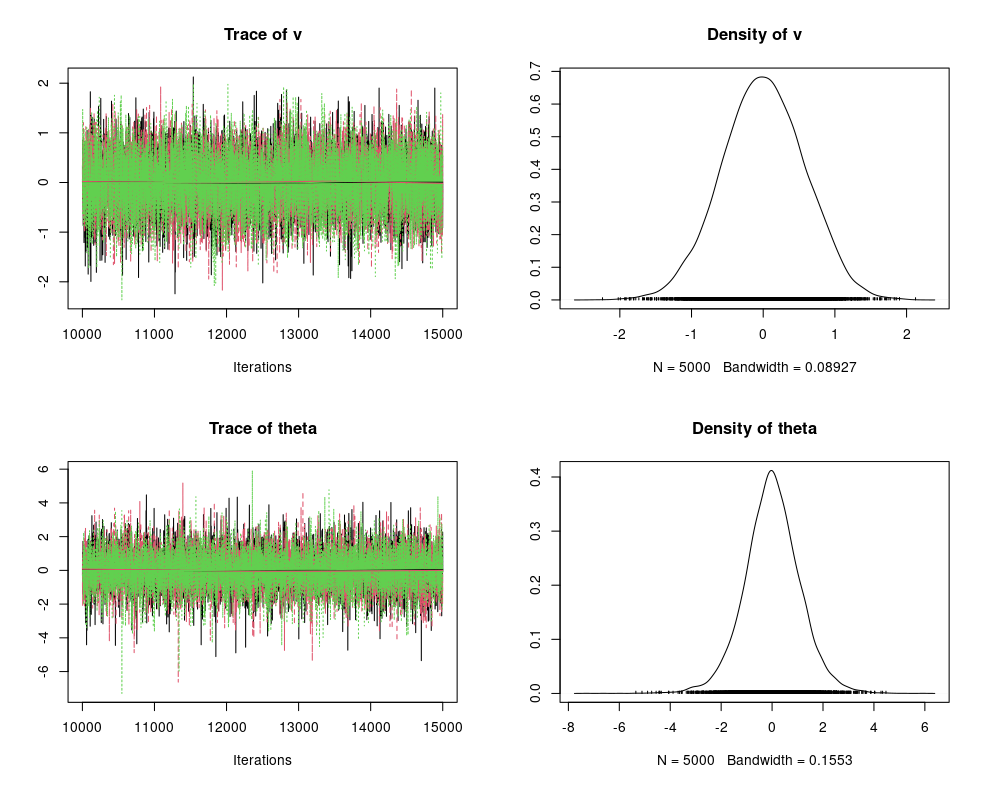
\includegraphics[width=0.7\linewidth]{1_jags_CE_simple}
	%
	\caption[The Devil's funnel. Centered Parametrization. JAGS]%
	{The Devil's funnel. Centered Parametrization implemented in JAGS. It shows the traceplot and distribution of the parameters of interest.}
	\label{fig:devil_CE_simple_jags}
\end{figure}
%
\begin{figure}[H]
	\centering
	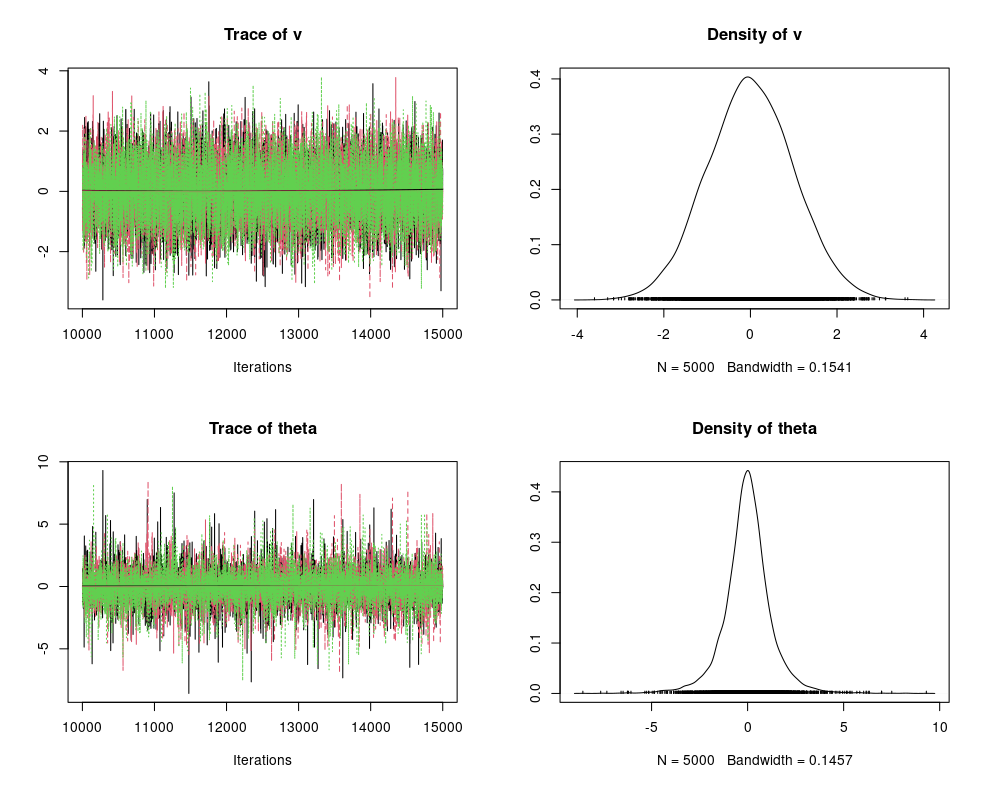
\includegraphics[width=0.7\linewidth]{2_jags_CE_priors}
	%
	\caption[The Devil's funnel. Centered Parametrization with mildly informative priors. JAGS]%
	{The Devil's funnel. Centered Parametrization with mildly informative priors implemented in JAGS. It shows the traceplot and distribution of the parameters of interest.}
	\label{fig:devil_CE_prior_jags}
\end{figure}
%
\begin{figure}[H]
	\centering
	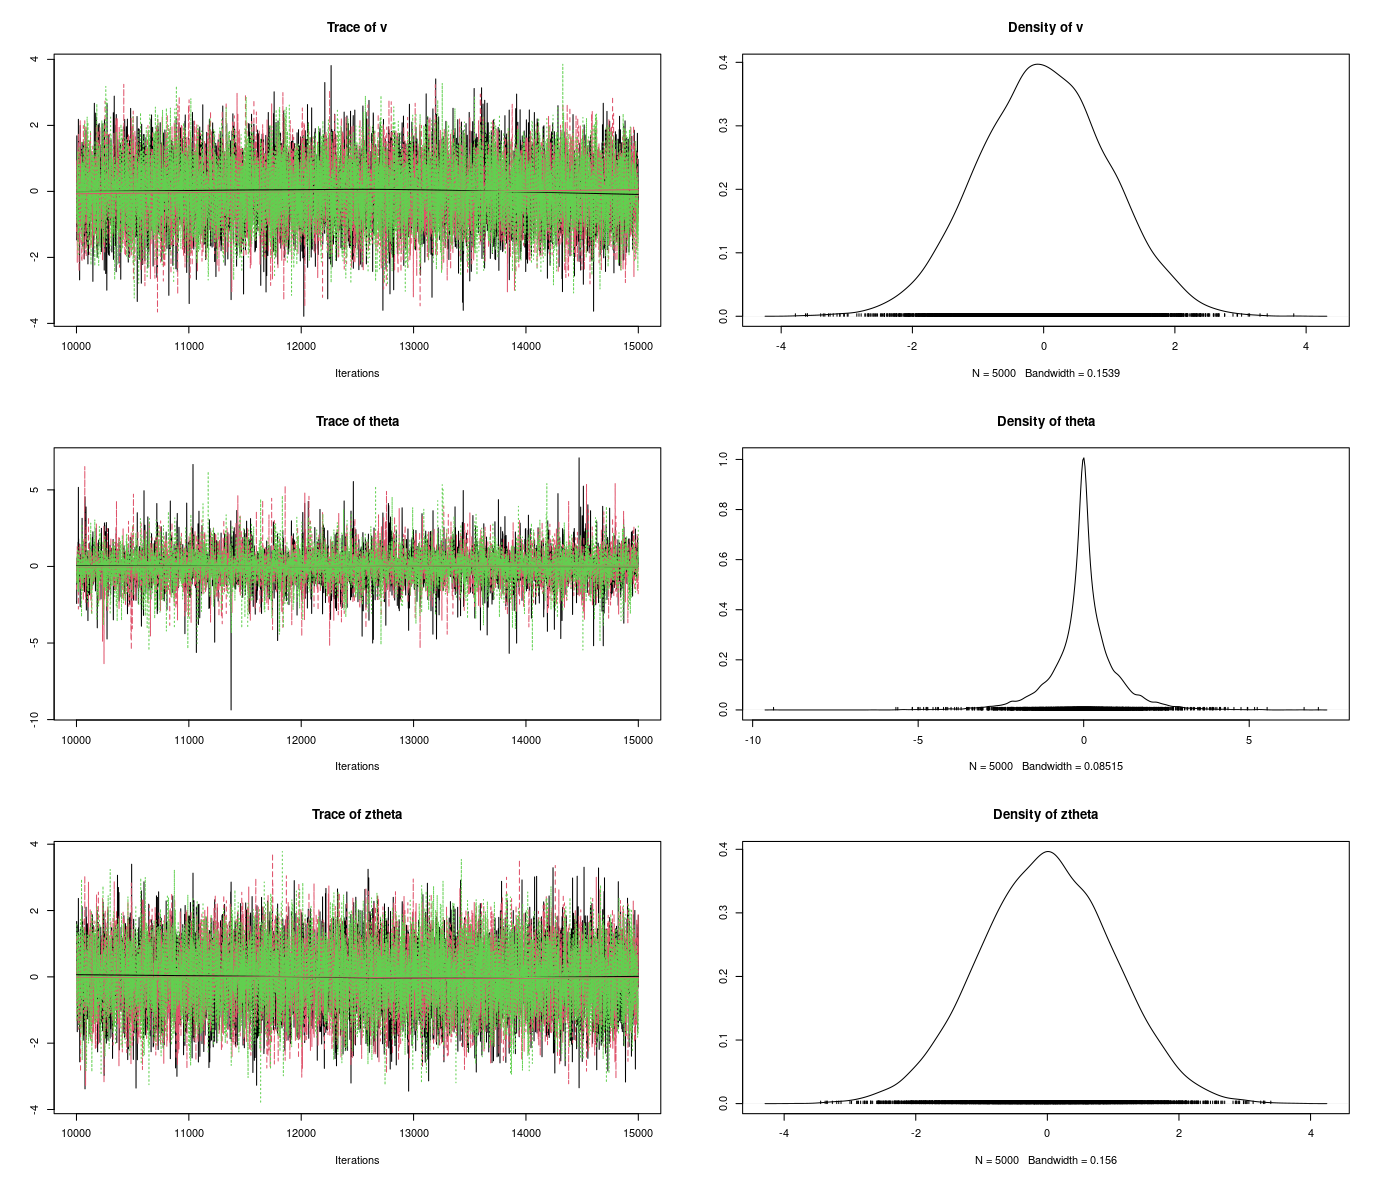
\includegraphics[width=0.7\linewidth]{3_jags_NC}
	%
	\caption[The Devil's funnel. Non-Centered Parametrization. JAGS]%
	{The Devil's funnel. Non-Centered Parametrization implemented in JAGS. It shows the traceplot and distribution of the parameters of interest.}
	\label{fig:devil_CE_NC_jags}
\end{figure}


%%%%%%%%%%%%%%%%%%%%%%%%%%%%%%%%%%%%%%%%%%%%%%%%%%%%%%%%%%%%%%%%%%%%%%%
%%%%%%%%%%%%%%%%%%%%%%%%%%%%%%%%%%%%%%%%%%%%%%%%%%%%%%%%%%%%%%%%%%%%%%%


\section{Chapter 4: Simulation study} \label{appB2:chapter4}

\subsection{Prior elicitation}
%
\begin{figure}[H]
	\centering
	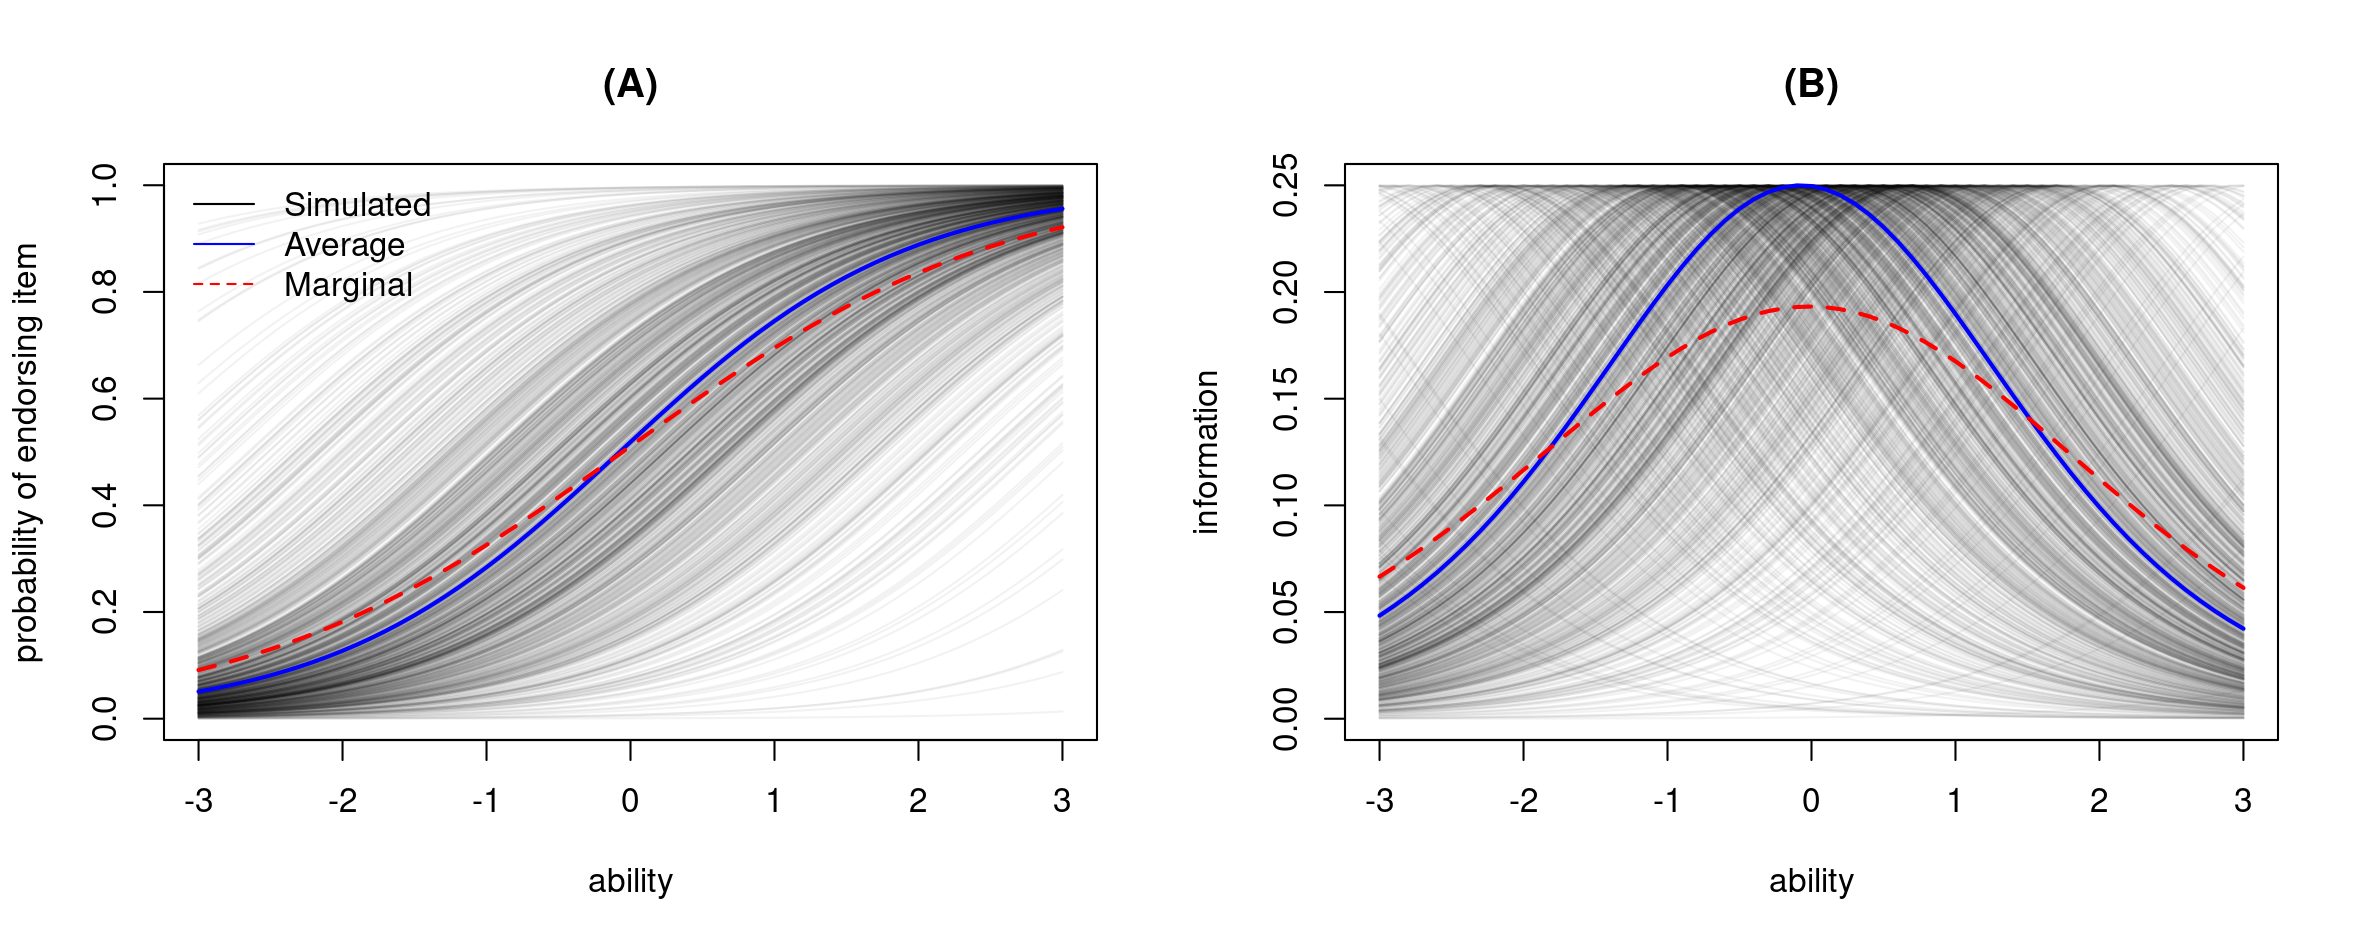
\includegraphics[width=1\linewidth]{SOLV_ICC_prior}
	%
	\caption[Second-order latent variable model (SOLV). Item Characteristic Curve (ICC) and Item Information Function (IIF).]%
	{Second-order latent variable model (SOLV). (A) Item Characteristics Curve, ICC. (B) Item Information Function, IIF.}
	\label{fig:SOLV_ICC_prior}
\end{figure}
%
\begin{figure}[H]
	\centering
	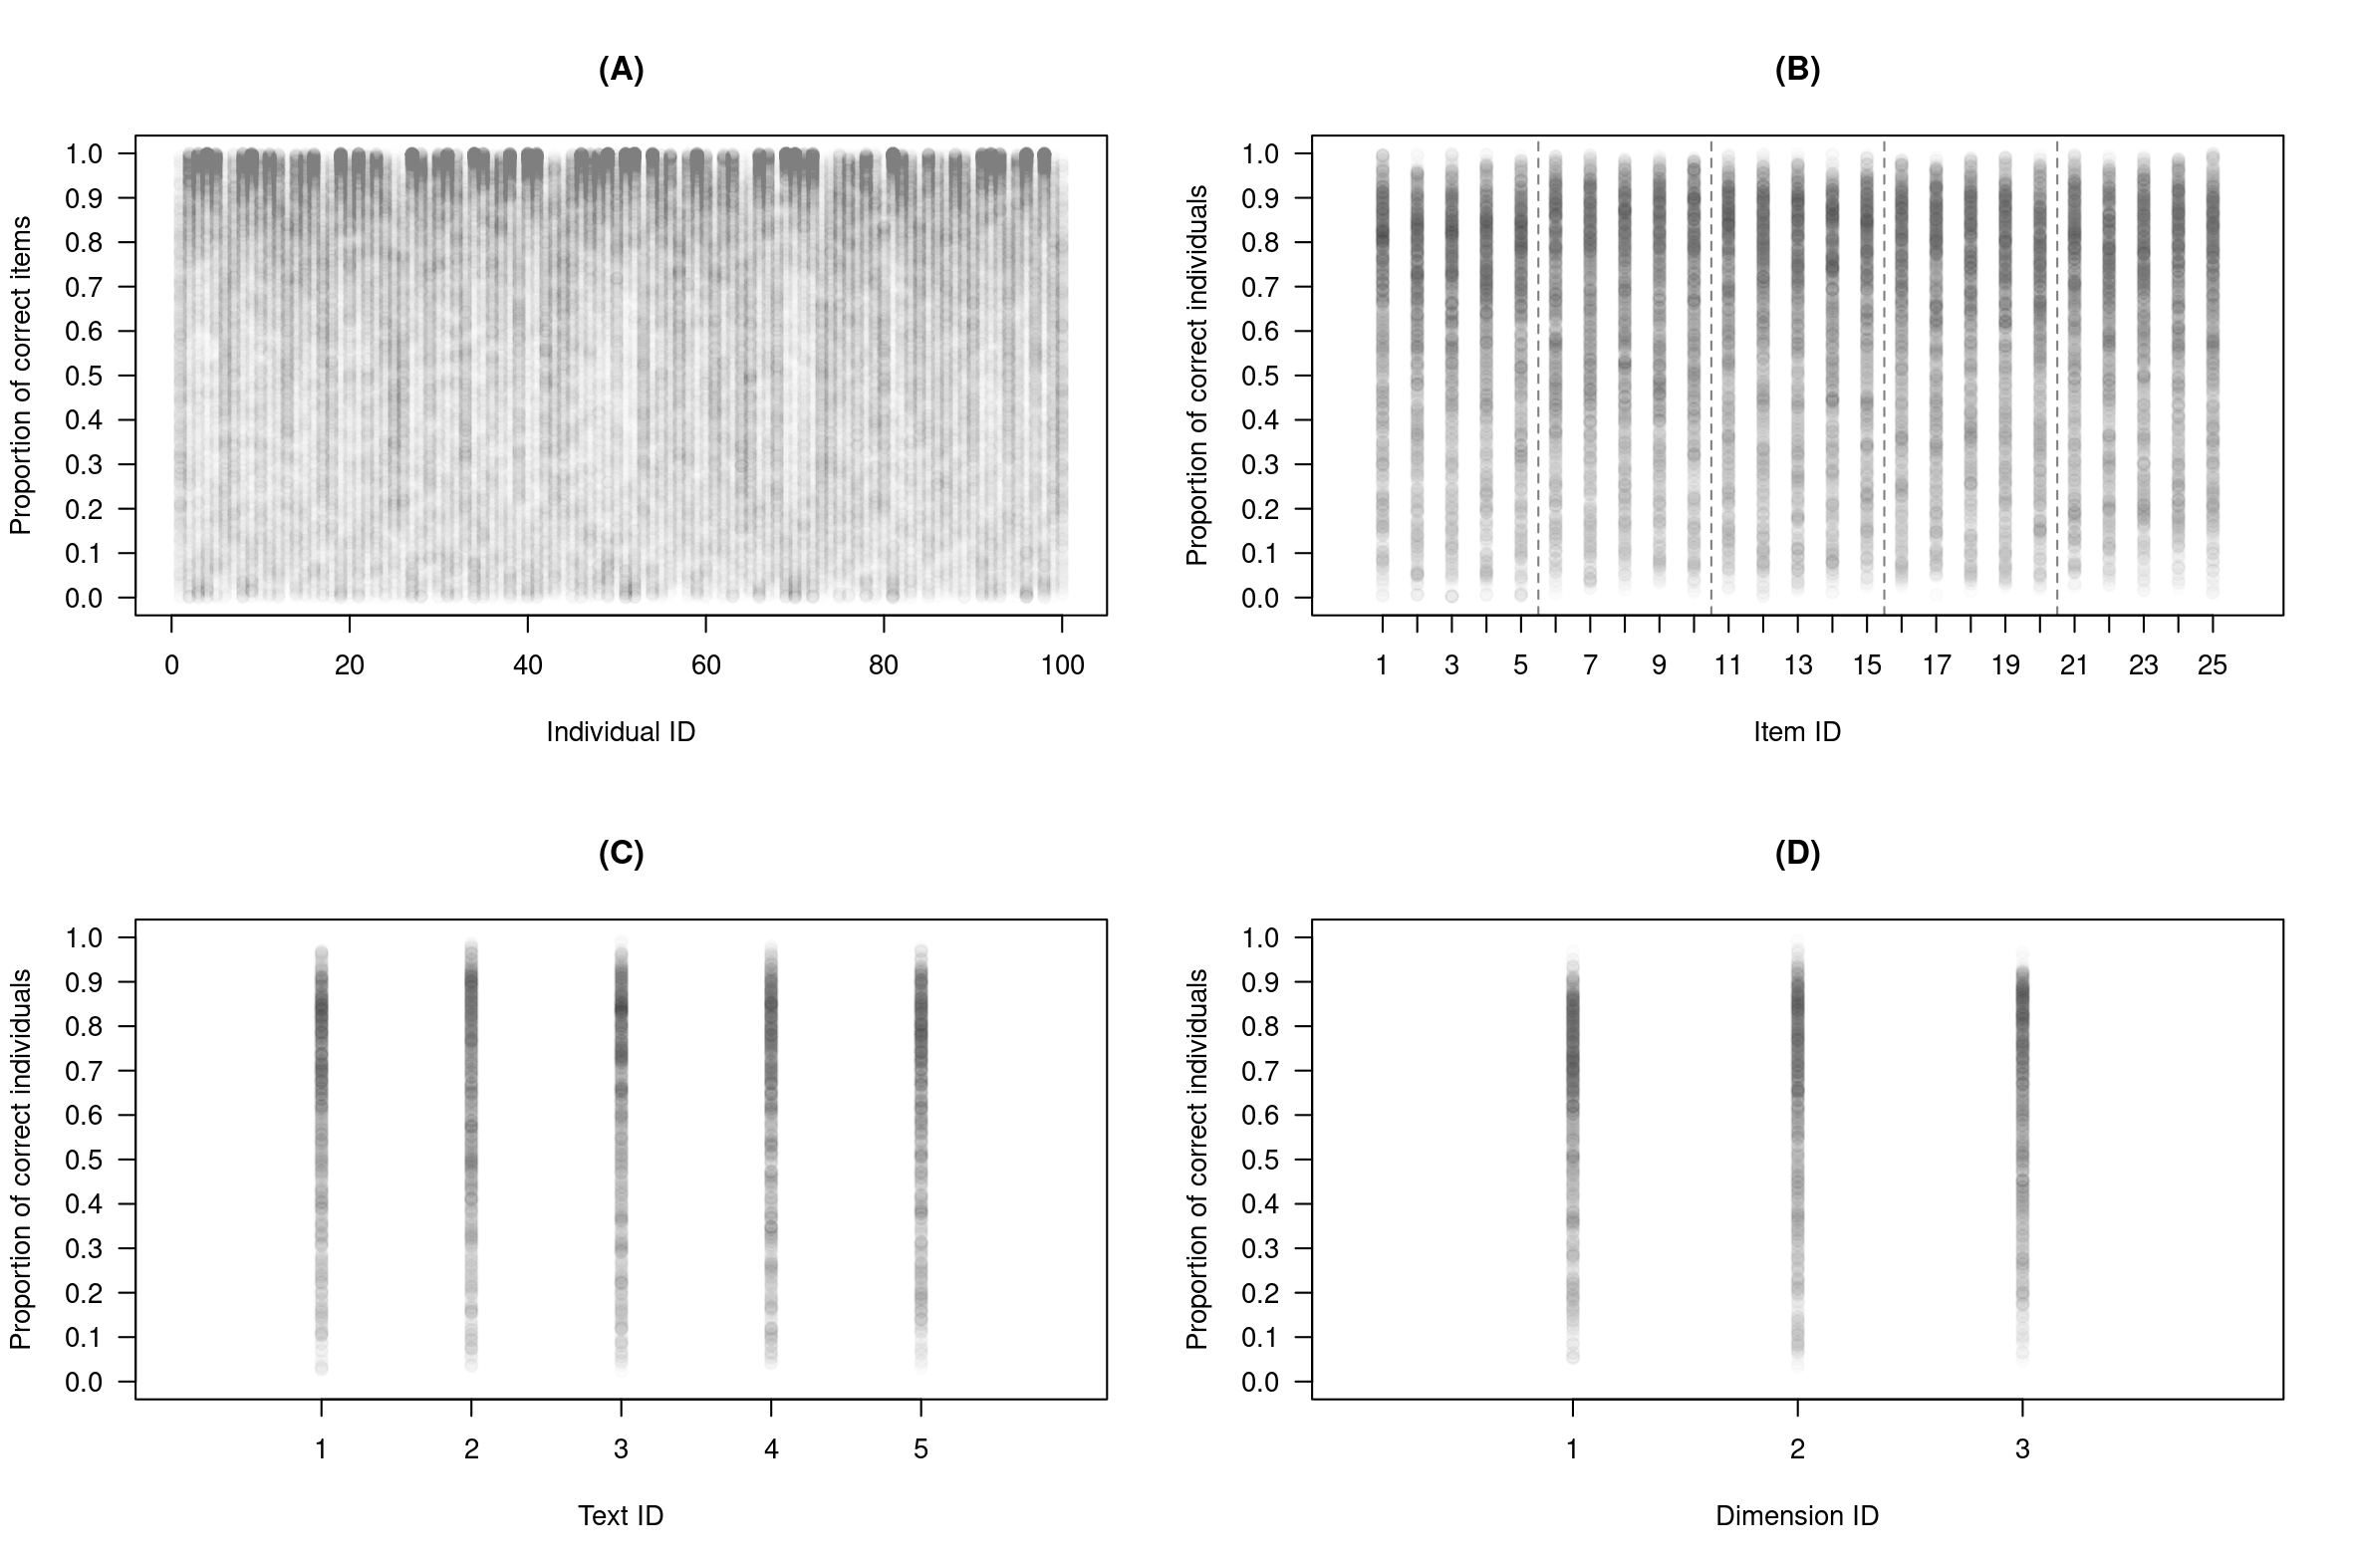
\includegraphics[width=1\linewidth]{SOLV_HitRate1}
	%
	\caption[Second-order latent variable model (SOLV). Hit rate per dimensions of interest.]%
	{Second-order latent variable model (SOLV). Aggregated endorsement rate per: (A) individuals, (B) items, (C) text or passage, and (D) measured dimension.}
	\label{fig:SOLV_hitrate1}
\end{figure}
%
\begin{figure}[H]
	\centering
	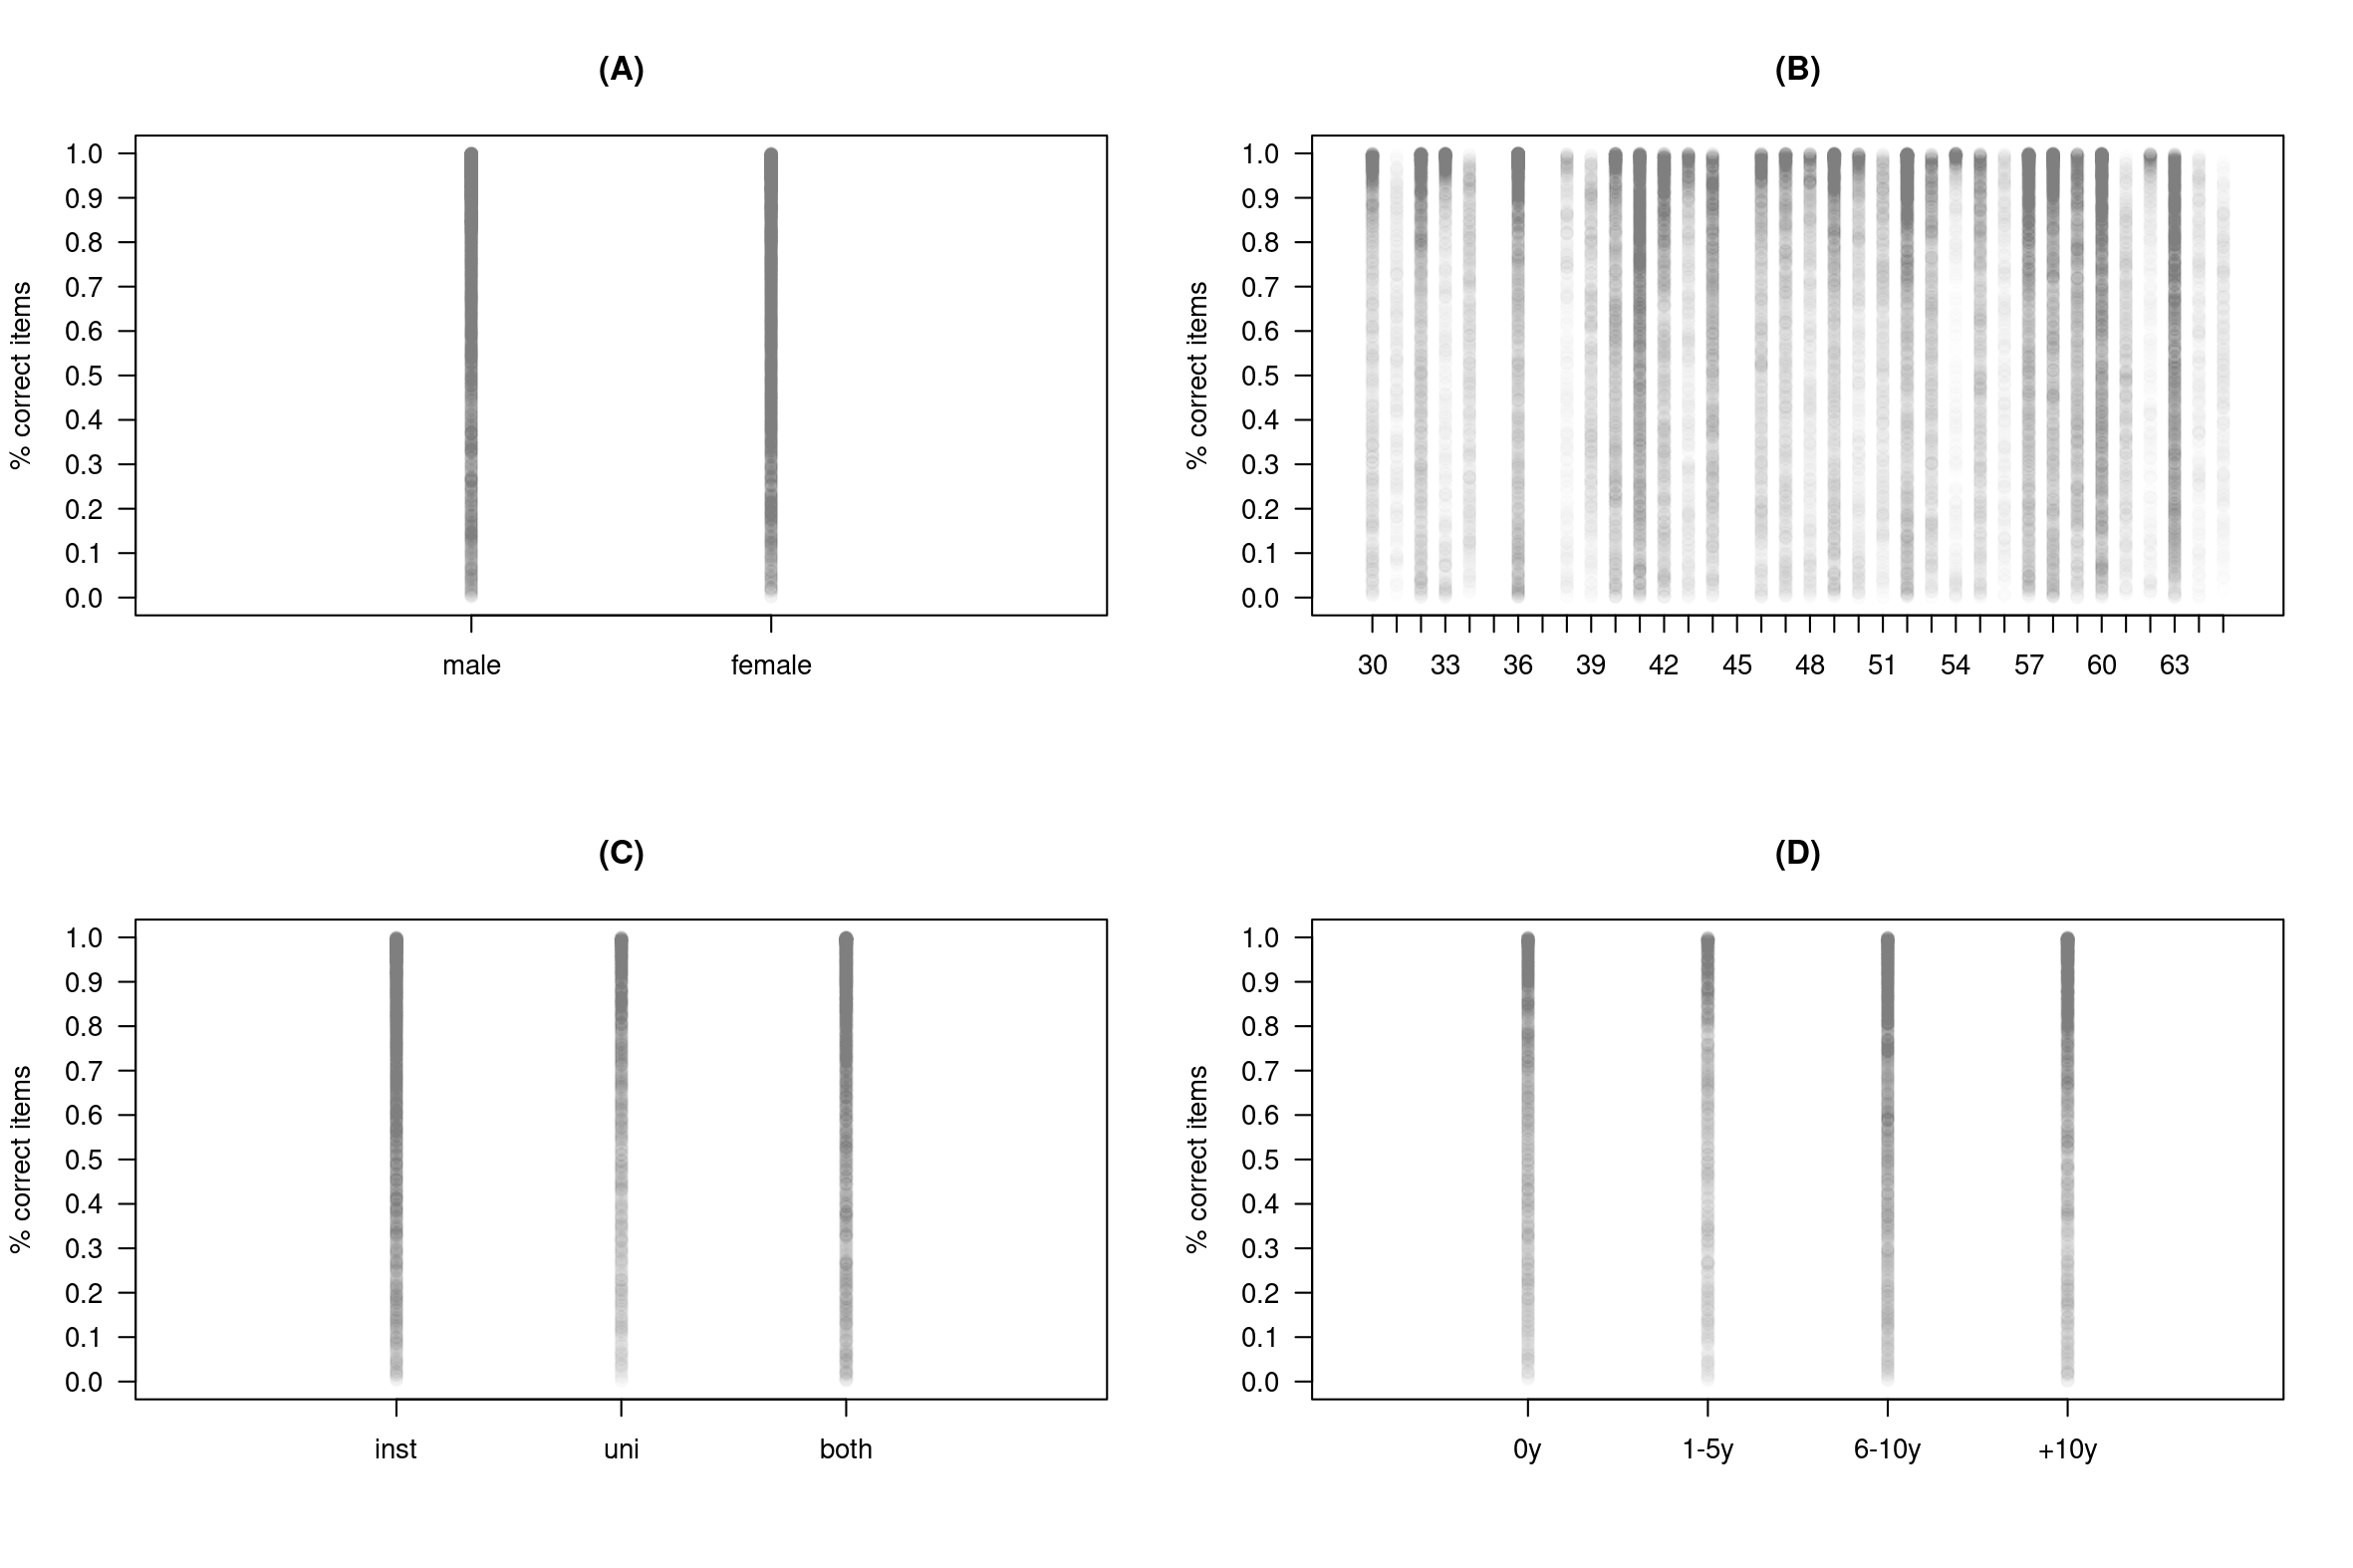
\includegraphics[width=1\linewidth]{SOLV_HitRate2}
	%
	\caption[Second-order latent variable model (SOLV). Hit rate per simulated covariate.]%
	{Second-order latent variable model (SOLV). Aggregated endorsement rate per simulated covariate: (A) gender, (B) age, (C) education, and (D) experience.}
	\label{fig:SOLV_hitrate2}
\end{figure}

%%%%%%%%%%%%%%%%%%%%%%%%%%%%%%%%%%%%%%%%%%%%%%%%%%%%%%%%%%%%%%%%%%%%%%%

\subsection{Chain performance} \label{sub_sect:chain_performance}

This section shows only a small set of trace, trank and ACF plots for the parameters of interest. For all the plots across parameters, models, parametrizations, and replicas refer to the ``chains" image section of the accompanying github page:

\noindent \url{https://github.com/jriveraespejo/thesis/tree/master/images/chains} \\

Similarly, the CP and NCP \texttt{n\_eff} and \texttt{Rhat} comparison plots shown here is a small set of the full available plots. For the set of figures across parameters, models, and replicas refer to the ``chains/stat" image section of the accompanying github page:

\noindent \url{https://github.com/jriveraespejo/thesis/tree/master/images/chains_stat}
%
\begin{figure}[H]
	\centering
	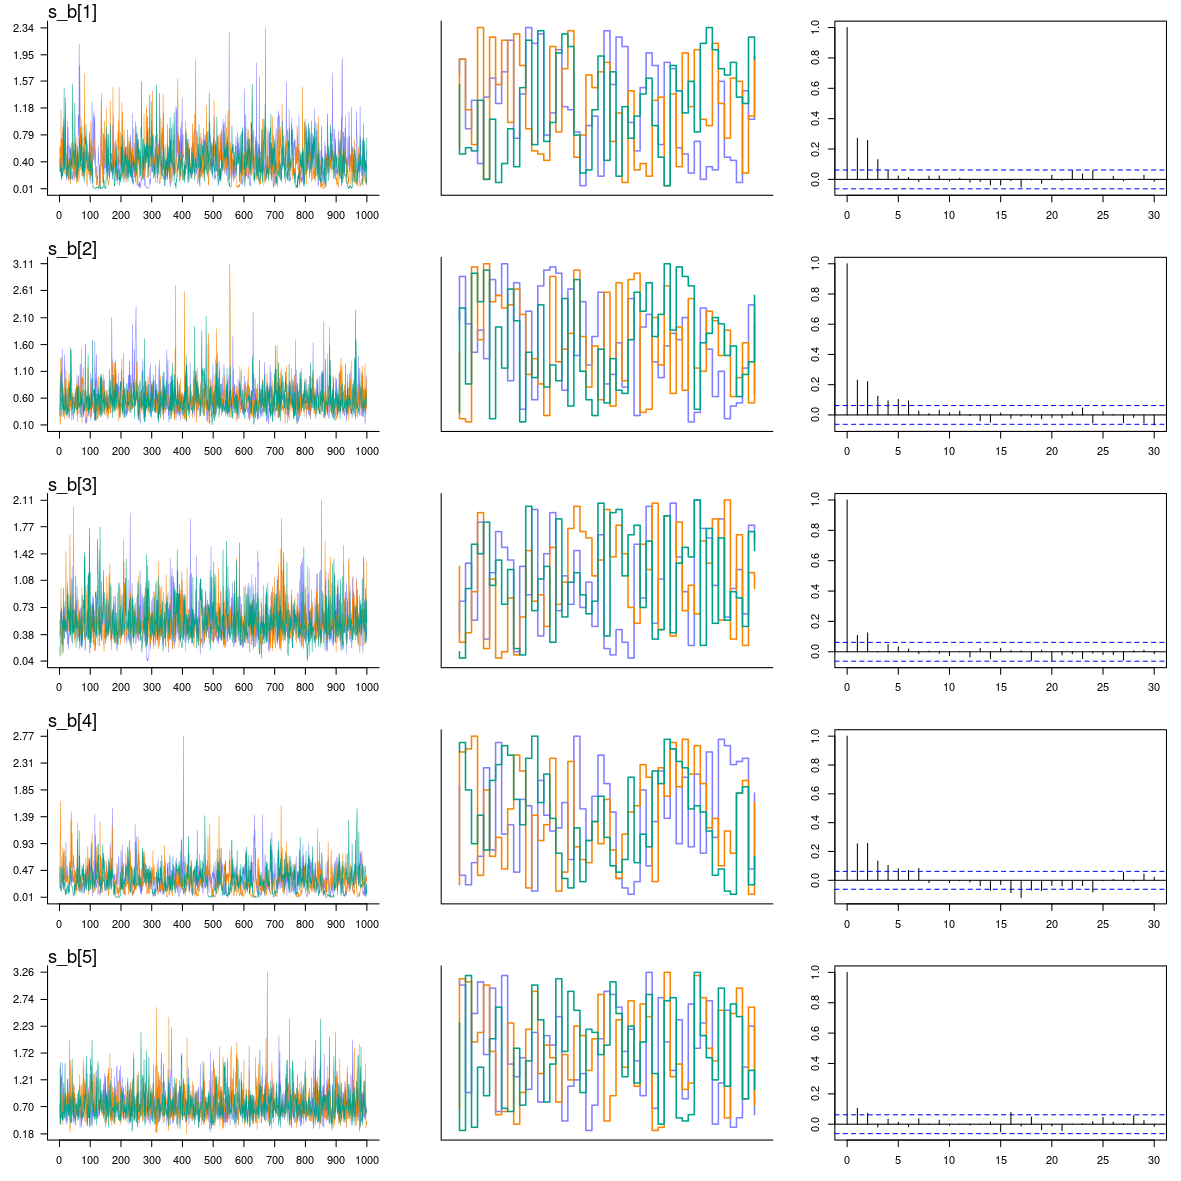
\includegraphics[width=1\linewidth]{FOLV_CE_J100_Ndata3_sb}
	%
	\caption[First-order latent variable model (FOLV). Sample size $100$, replica number $3$. Centered parametrization. Difficulty deviation per text. Trace, trank and auto-correlation plots.]%
	{First-order latent variable model (FOLV). Sample size $100$, replica number $3$. Centered parametrization. Difficulty deviation per text: (Left) trace plot, (Middle) trank plot, (Right) auto-correlation plot.}
	\label{fig:FOLV_CE_chains2}
\end{figure}
%
\begin{figure}[H]
	\centering
	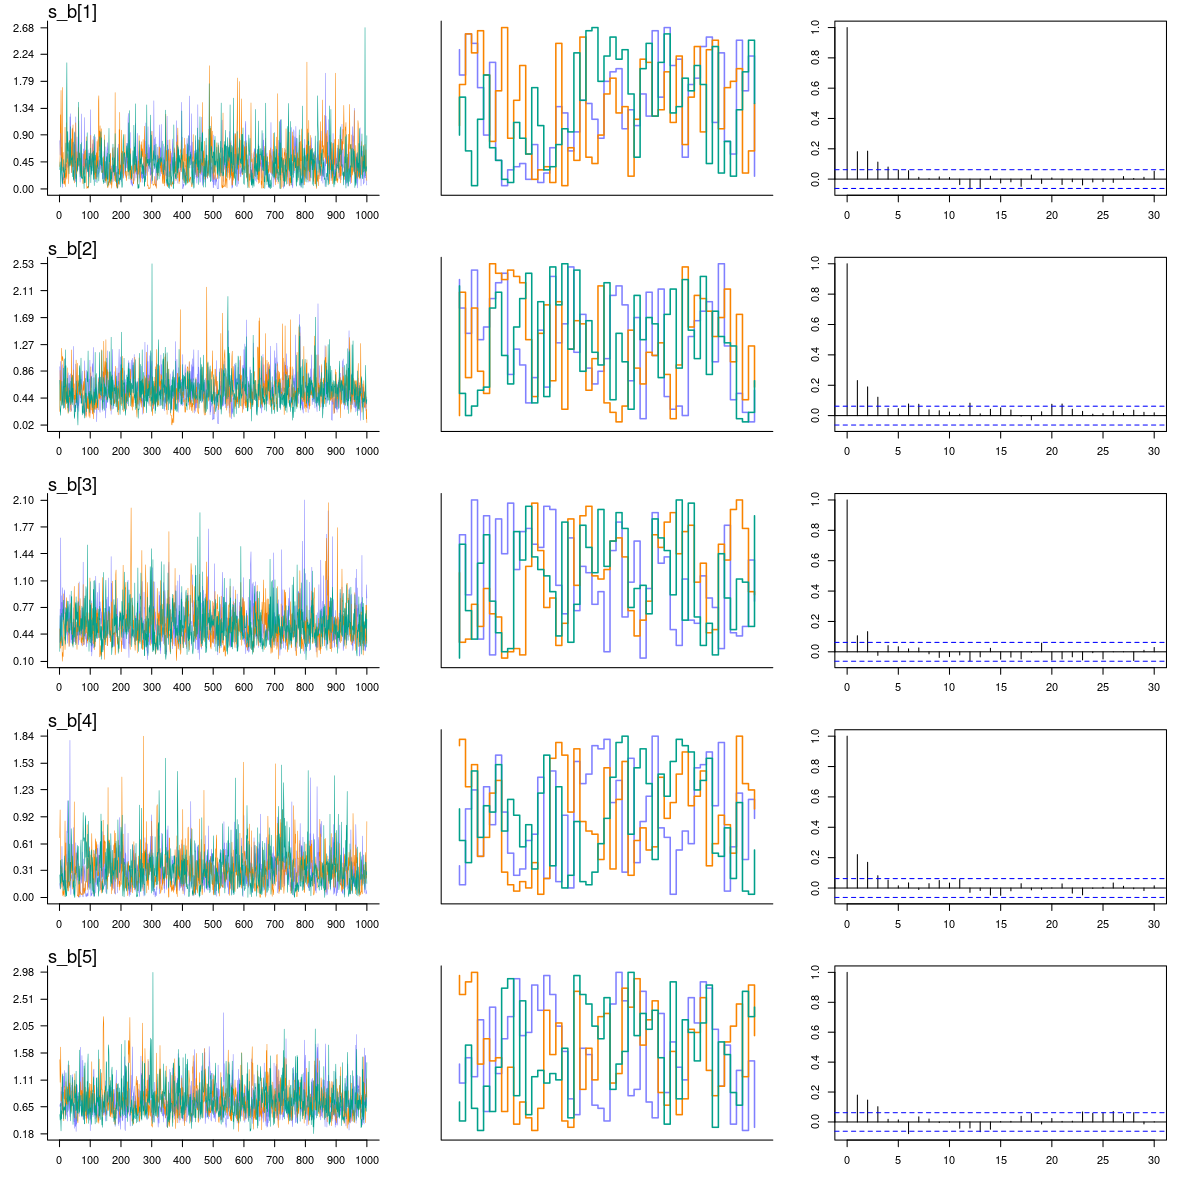
\includegraphics[width=1\linewidth]{FOLV_NC_J100_Ndata3_sb}
	%
	\caption[First-order latent variable model (FOLV). Sample size $100$, replica number $3$. Non-centered parametrization. Difficulty deviation per text. Trace, trank and auto-correlation plots.]%
	{First-order latent variable model (FOLV). Sample size $100$, replica number $3$. Non-centered parametrization. Difficulty deviation per text: (Left) trace plot, (Middle) trank plot, (Right) auto-correlation plot.}
	\label{fig:FOLV_NC_chains2}
\end{figure}
%
\begin{figure}[H]
	\centering
	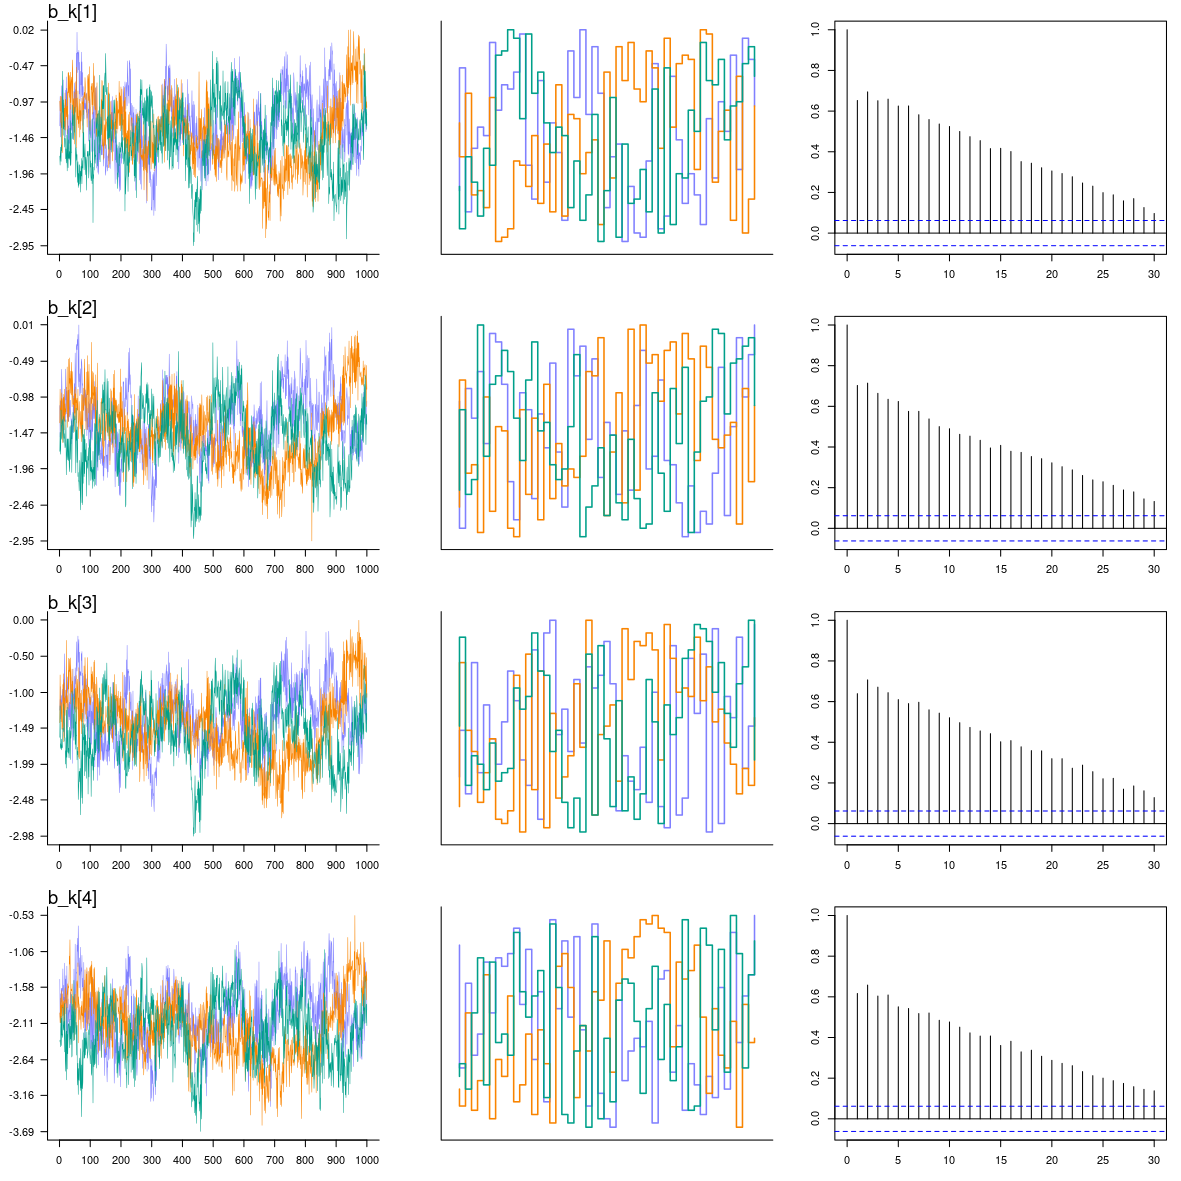
\includegraphics[width=1\linewidth]{FOLV_CE_J100_Ndata1_bk1}
	%
	\caption[First-order latent variable model (FOLV). Sample size $100$, replica number $1$. Centered parametrization. Difficulty per item. Trace, trank and auto-correlation plots.]%
	{First-order latent variable model (FOLV). Sample size $100$, replica number $1$. Centered parametrization. Difficulty per item: (Left) trace plot, (Middle) trank plot, (Right) auto-correlation plot.}
	\label{fig:FOLV_CE_chains3}
\end{figure}
%
\begin{figure}[H]
	\centering
	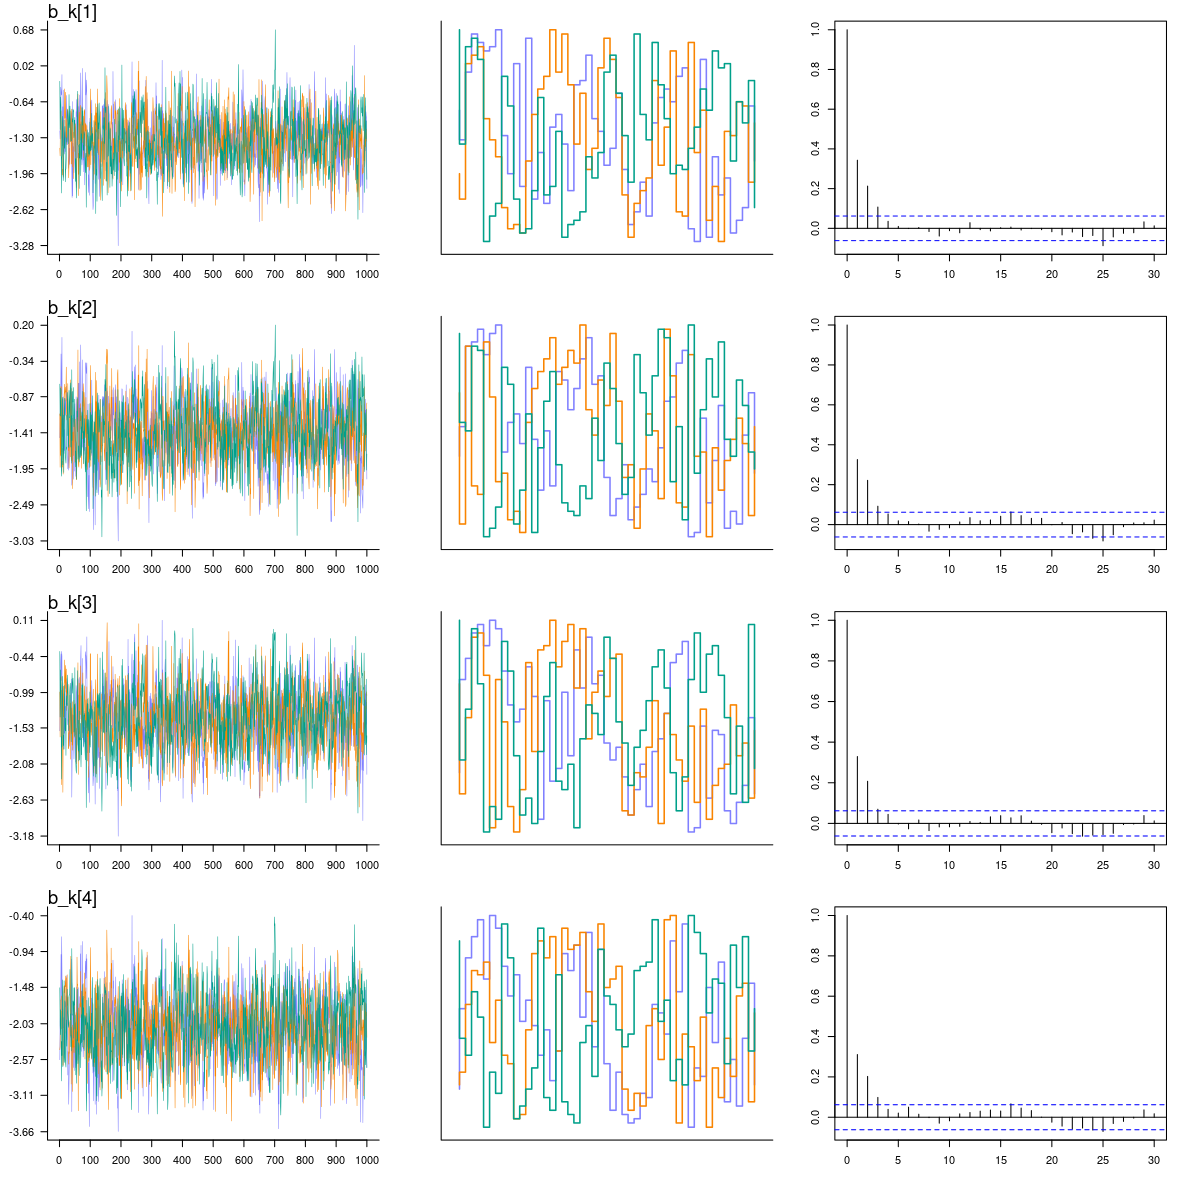
\includegraphics[width=1\linewidth]{FOLV_NC_J100_Ndata1_bk1}
	%
	\caption[First-order latent variable model (FOLV). Sample size $100$, replica number $1$. Non-centered parametrization. Difficulty per item. Trace, trank and auto-correlation plots.]%
	{First-order latent variable model (FOLV). Sample size $100$, replica number $1$. Non-centered parametrization. Difficulty per item: (Left) trace plot, (Middle) trank plot, (Right) auto-correlation plot.}
	\label{fig:FOLV_NC_chains3}
\end{figure}
%
\begin{figure}[H]
	\centering
	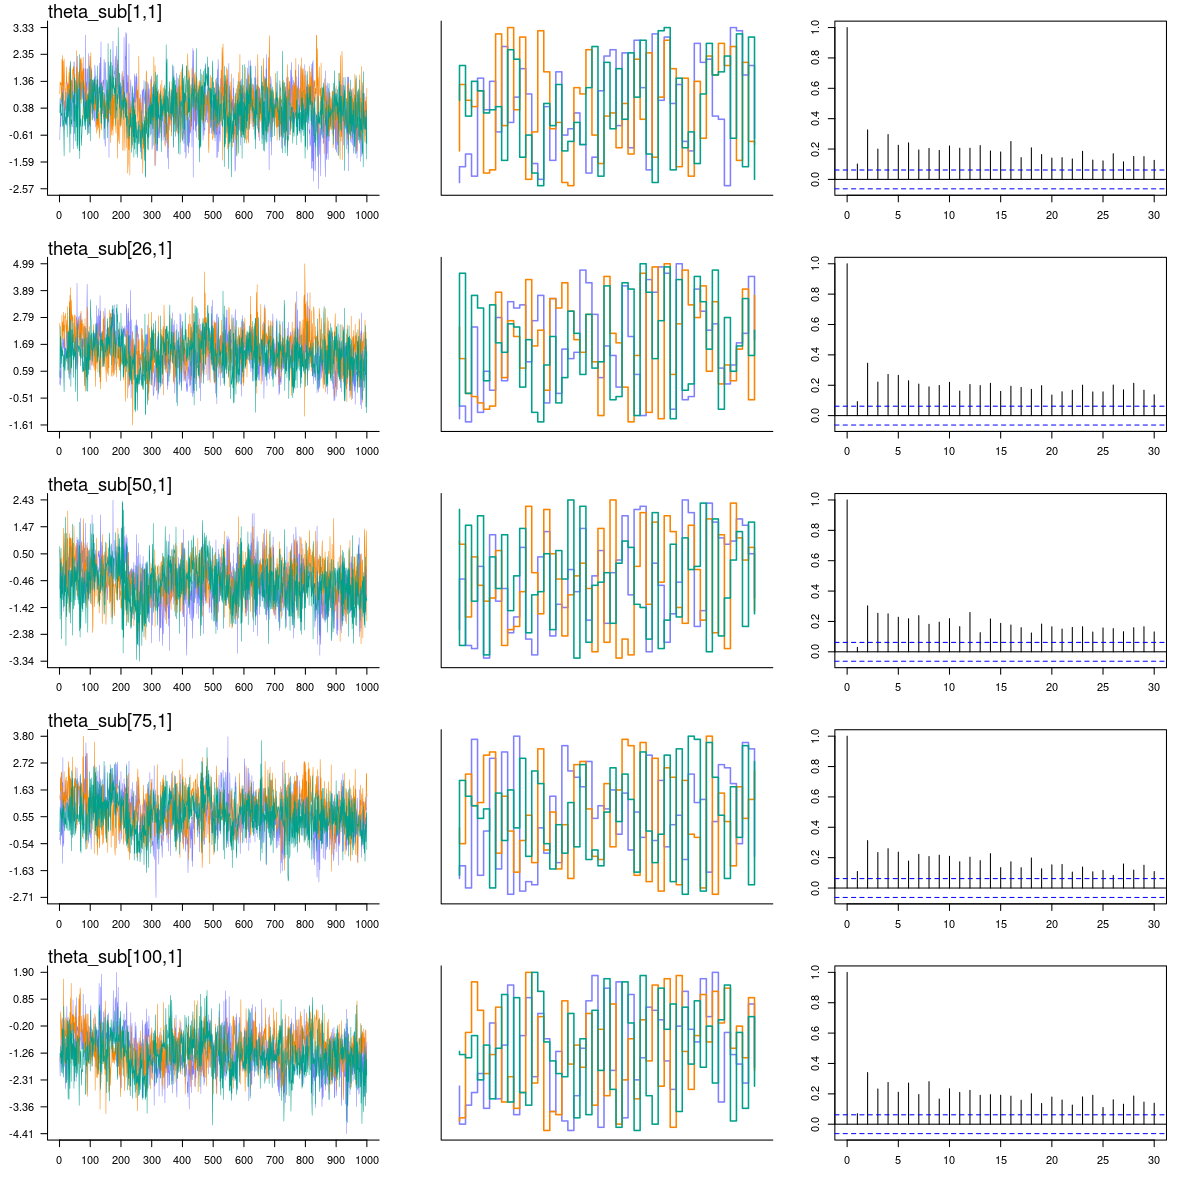
\includegraphics[width=1\linewidth]{FOLV_CE_J100_Ndata6_theta_sub1}
	%
	\caption[First-order latent variable model (FOLV). Sample size $100$, replica number $6$. Centered parametrization. Individual's first sub-dimension. Trace, trank and auto-correlation plots.]%
	{First-order latent variable model (FOLV). Sample size $100$, replica number $6$. Centered parametrization. Individual's first sub-dimension: (Left) trace plot, (Middle) trank plot, (Right) auto-correlation plot.}
	\label{fig:FOLV_CE_chains4}
\end{figure}
%
\begin{figure}[H]
	\centering
	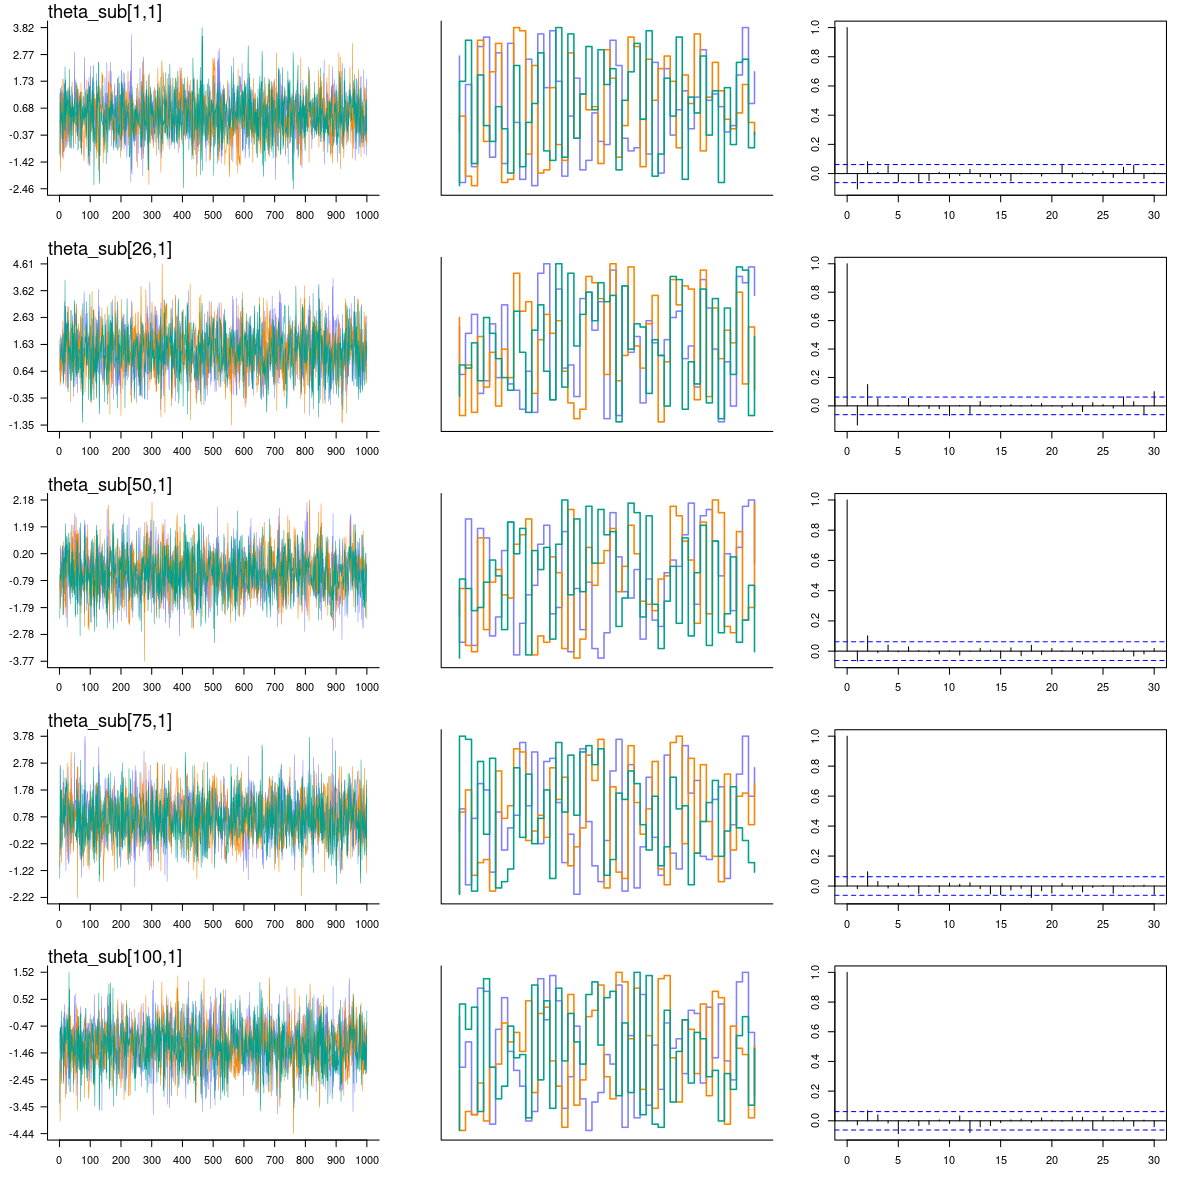
\includegraphics[width=1\linewidth]{FOLV_NC_J100_Ndata6_theta_sub1}
	%
	\caption[First-order latent variable model (FOLV). Sample size $100$, replica number $6$. Non-centered parametrization. Individual's first sub-dimension. Trace, trank and auto-correlation plots.]%
	{First-order latent variable model (FOLV). Sample size $100$, replica number $6$. Non-centered parametrization. Individual's first sub-dimension: (Left) trace plot, (Middle) trank plot, (Right) auto-correlation plot.}
	\label{fig:FOLV_NC_chains4}
\end{figure}
%
\begin{figure}[H]
	\centering
	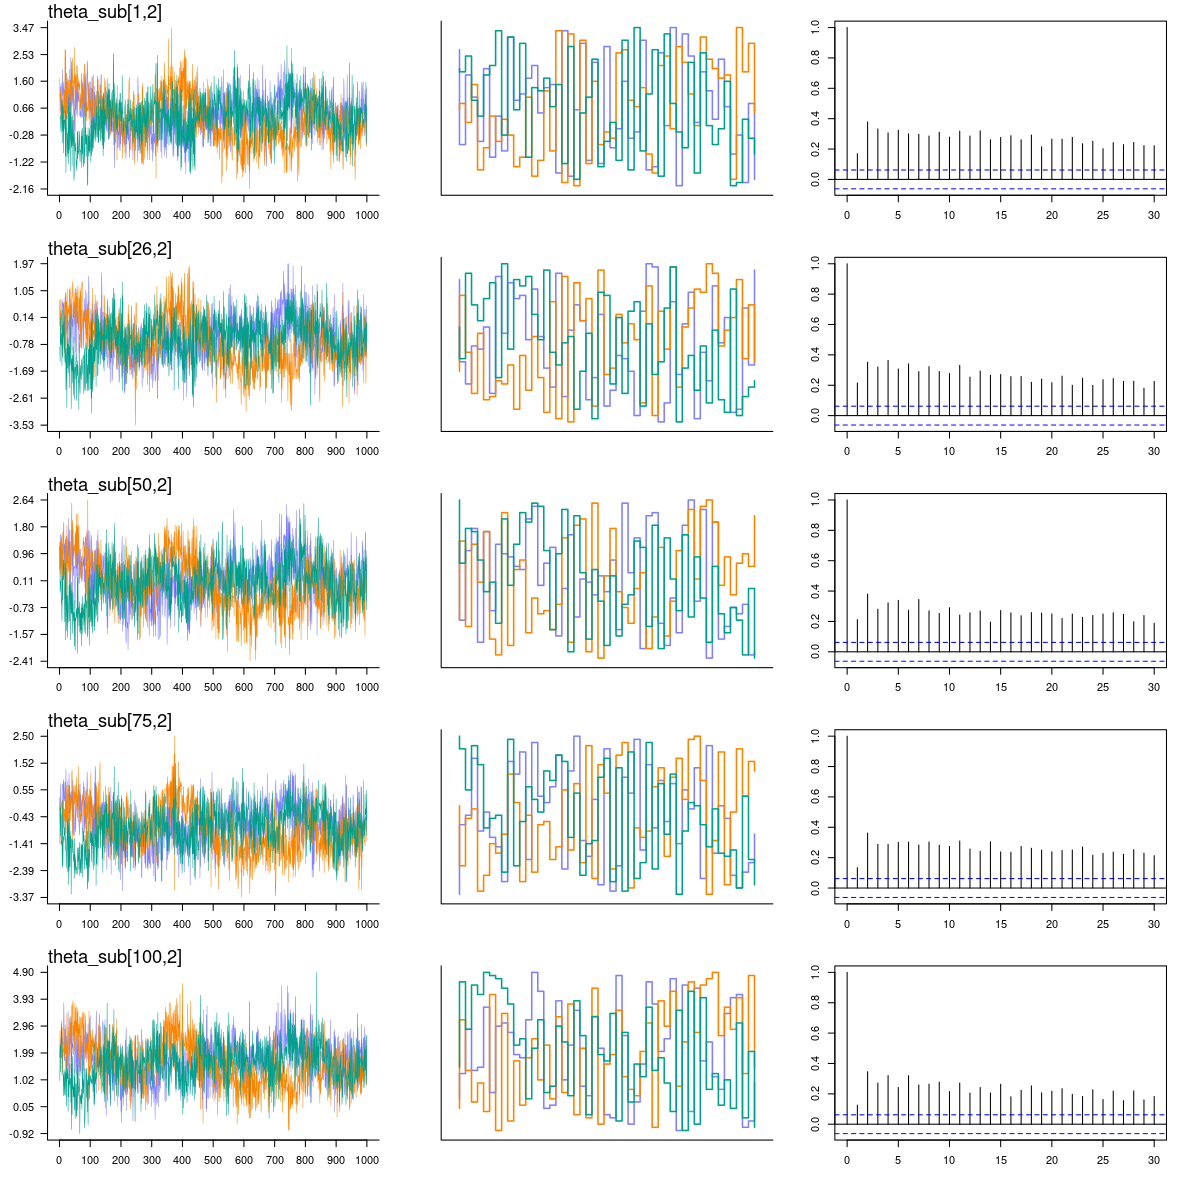
\includegraphics[width=1\linewidth]{FOLV_CE_J100_Ndata7_theta_sub2}
	%
	\caption[First-order latent variable model (FOLV). Sample size $100$, replica number $7$. Centered parametrization. Individual's second sub-dimension. Trace, trank and auto-correlation plots.]%
	{First-order latent variable model (FOLV). Sample size $100$, replica number $7$. Centered parametrization. Individual's second sub-dimension: (Left) trace plot, (Middle) trank plot, (Right) auto-correlation plot.}
	\label{fig:FOLV_CE_chains5}
\end{figure}
%
\begin{figure}[H]
	\centering
	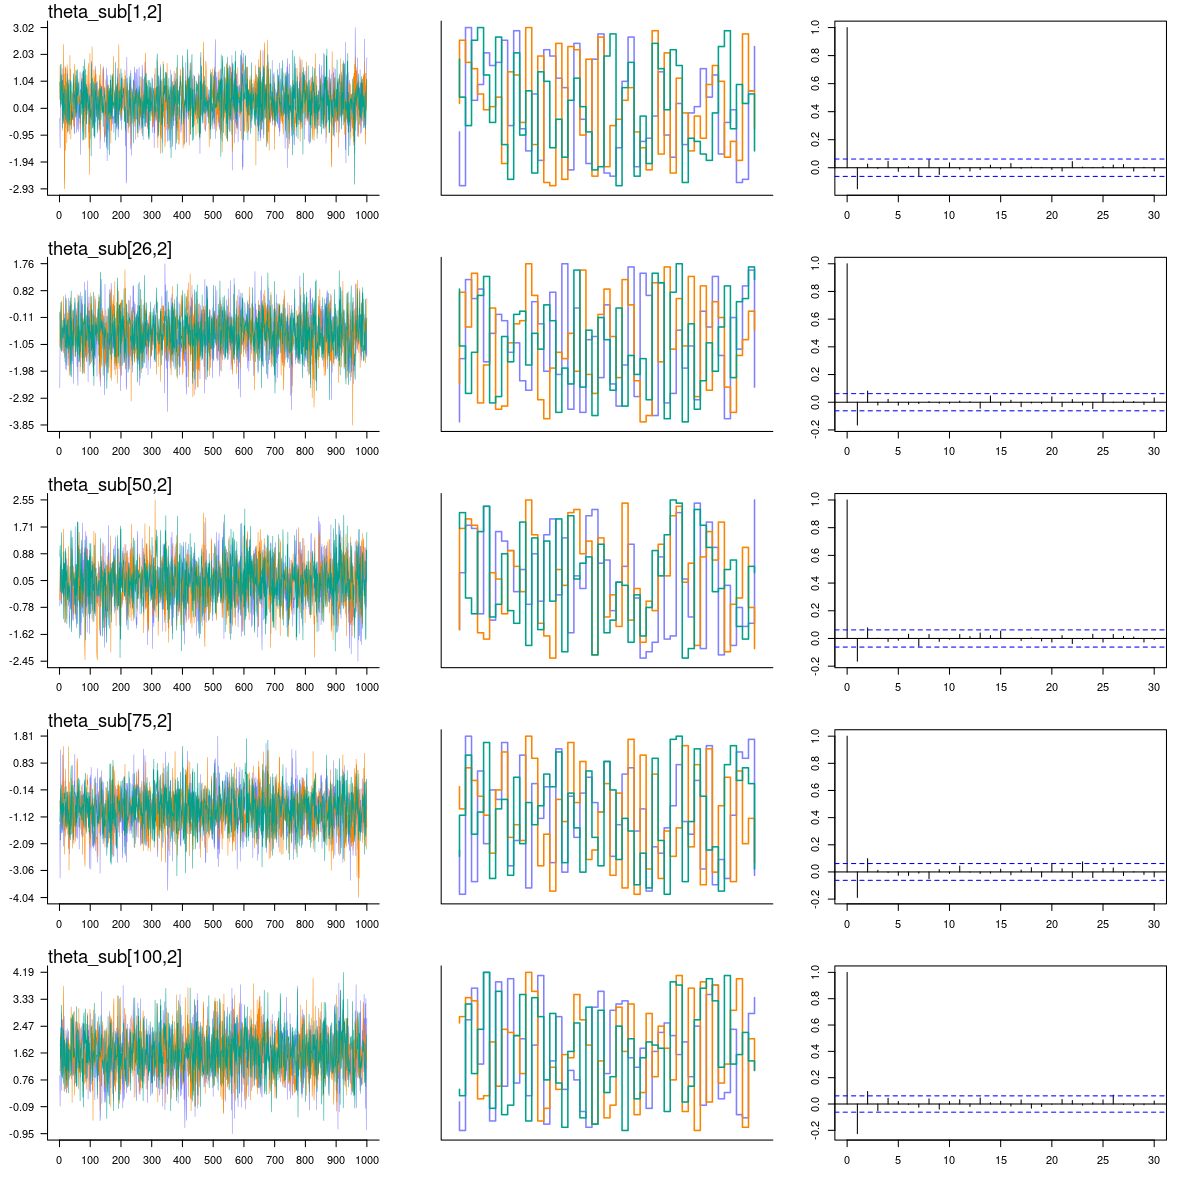
\includegraphics[width=1\linewidth]{FOLV_NC_J100_Ndata7_theta_sub2}
	%
	\caption[First-order latent variable model (FOLV). Sample size $100$, replica number $7$. Non-centered parametrization. Individual's second sub-dimension. Trace, trank and auto-correlation plots.]%
	{First-order latent variable model (FOLV). Sample size $100$, replica number $7$. Non-centered parametrization. Individual's second sub-dimension: (Left) trace plot, (Middle) trank plot, (Right) auto-correlation plot.}
	\label{fig:FOLV_NC_chains5}
\end{figure}
%
\begin{figure}[H]
	\centering
	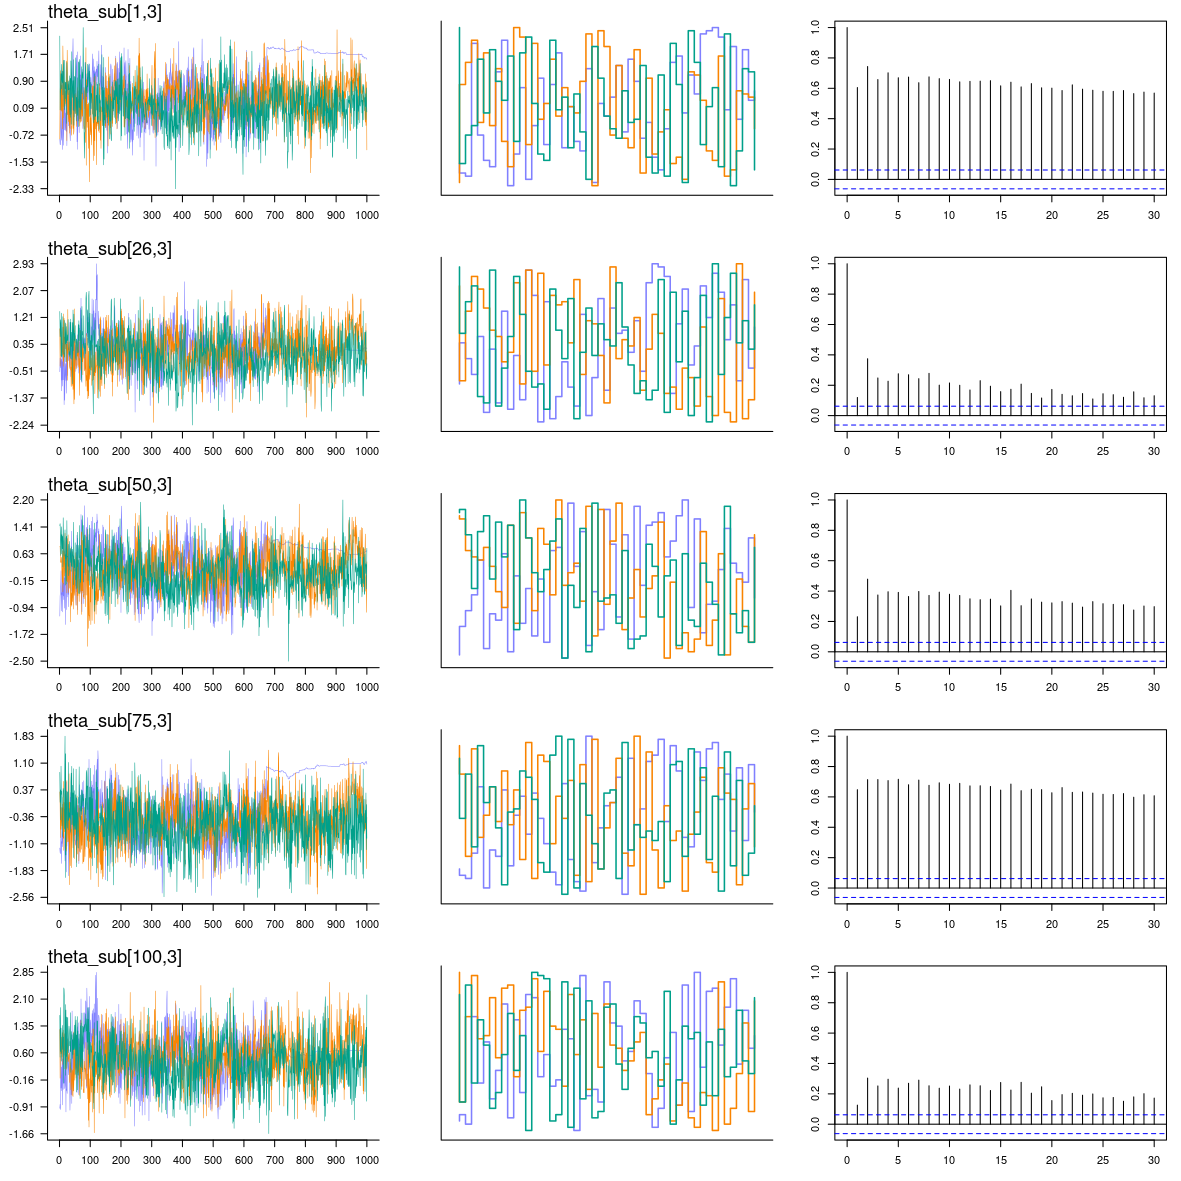
\includegraphics[width=1\linewidth]{FOLV_CE_J100_Ndata8_theta_sub3}
	%
	\caption[First-order latent variable model (FOLV). Sample size $100$, replica number $8$. Centered parametrization. Individual's third sub-dimension. Trace, trank and auto-correlation plots.]%
	{First-order latent variable model (FOLV). Sample size $100$, replica number $8$. Centered parametrization. Individual's third sub-dimension: (Left) trace plot, (Middle) trank plot, (Right) auto-correlation plot.}
	\label{fig:FOLV_CE_chains6}
\end{figure}
%
\begin{figure}[H]
	\centering
	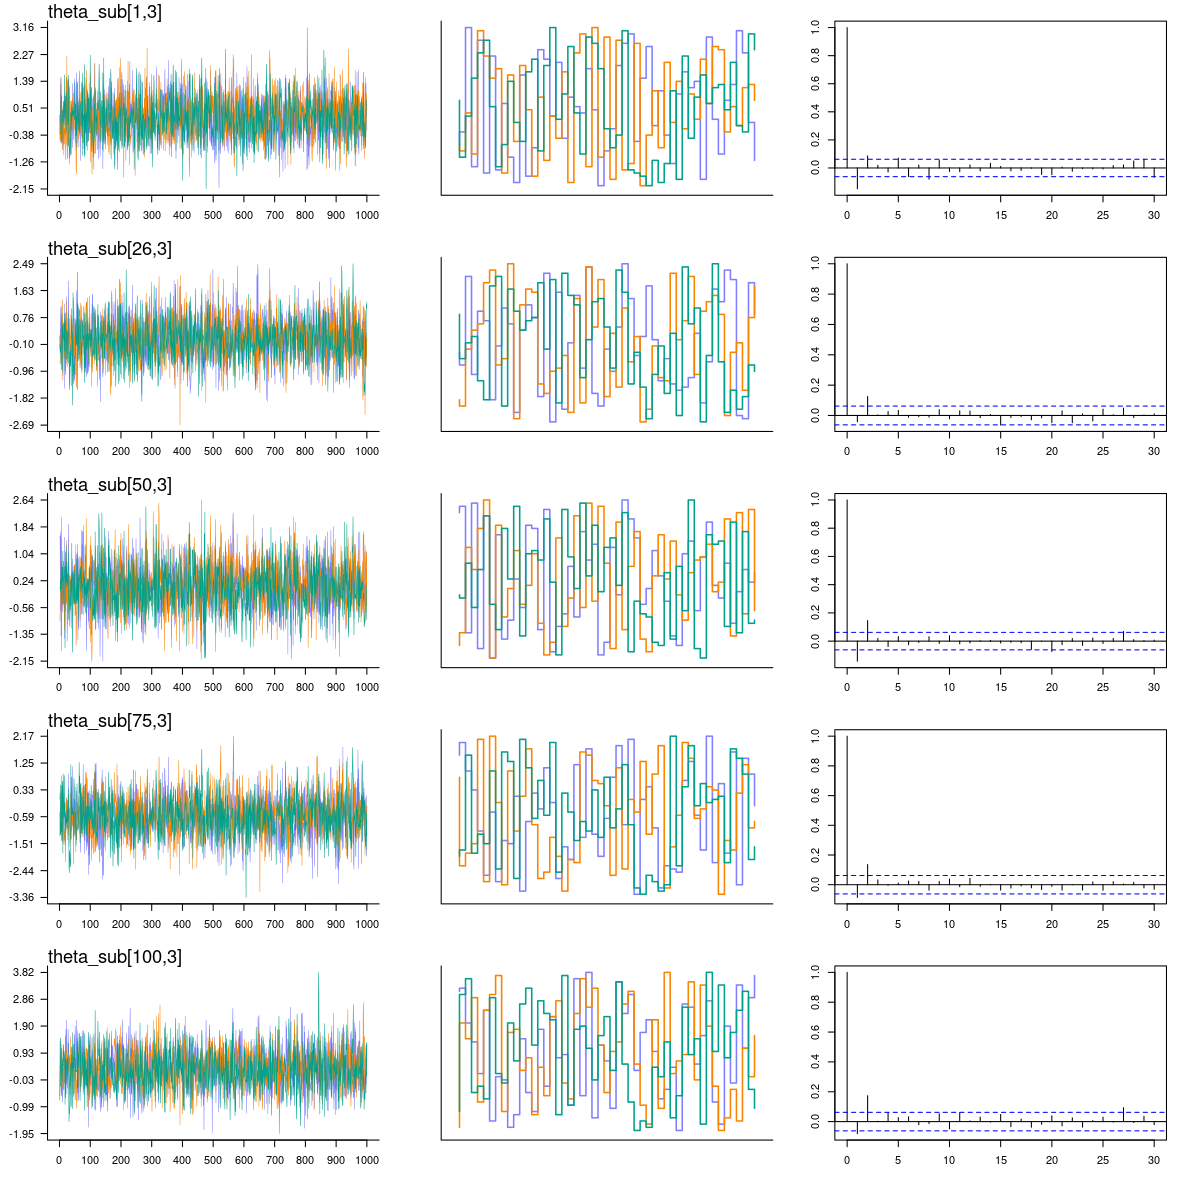
\includegraphics[width=1\linewidth]{FOLV_NC_J100_Ndata8_theta_sub3}
	%
	\caption[First-order latent variable model (FOLV). Sample size $100$, replica number $8$. Non-centered parametrization. Individual's third sub-dimension. Trace, trank and auto-correlation plots.]%
	{First-order latent variable model (FOLV). Sample size $100$, replica number $8$. Non-centered parametrization. Individual's third sub-dimension: (Left) trace plot, (Middle) trank plot, (Right) auto-correlation plot.}
	\label{fig:FOLV_NC_chains6}
\end{figure}
%
\begin{figure}[H]
	\centering
	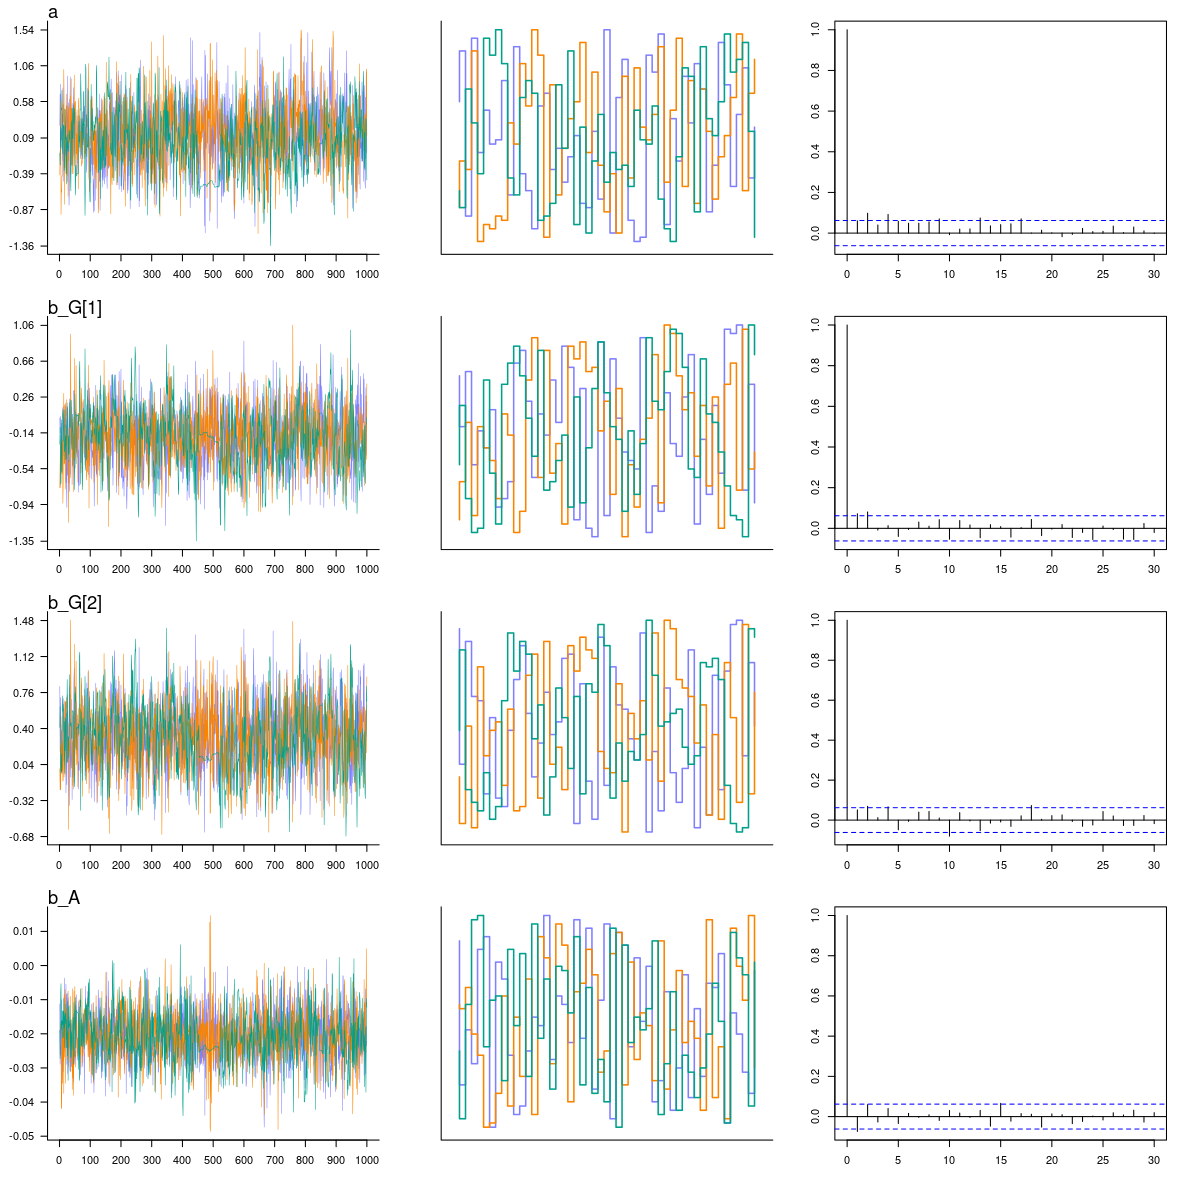
\includegraphics[width=1\linewidth]{FOLV_CE_J100_Ndata4_reg1}
	%
	\caption[First-order latent variable model (FOLV). Sample size $100$, replica number $4$. Centered parametrization. Regression parameters. Trace, trank and auto-correlation plots.]%
	{First-order latent variable model (FOLV). Sample size $100$, replica number $4$. Centered parametrization. Regression parameters: (Left) trace plot, (Middle) trank plot, (Right) auto-correlation plot.}
	\label{fig:FOLV_CE_chains7}
\end{figure}
%
\begin{figure}[H]
	\centering
	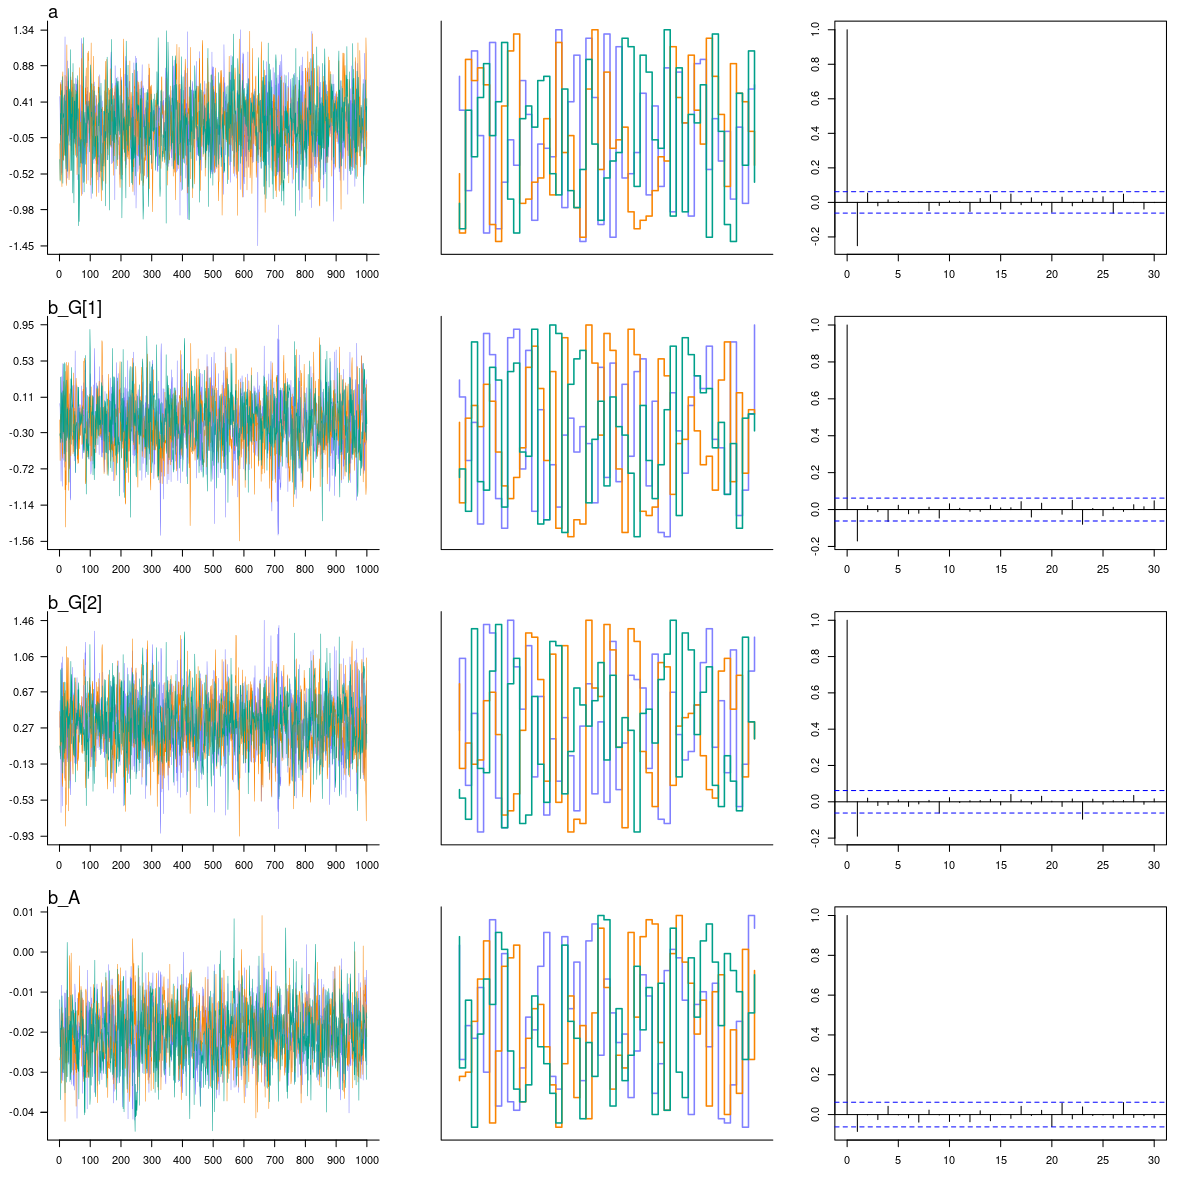
\includegraphics[width=1\linewidth]{FOLV_NC_J100_Ndata4_reg1}
	%
	\caption[First-order latent variable model (FOLV). Sample size $100$, replica number $4$. Non-centered parametrization. Regression parameters. Trace, trank and auto-correlation plots.]%
	{First-order latent variable model (FOLV). Sample size $100$, replica number $4$. Non-centered parametrization. Regression parameters: (Left) trace plot, (Middle) trank plot, (Right) auto-correlation plot.}
	\label{fig:FOLV_NC_chains7}
\end{figure}
%
\begin{figure}[H]
	\centering
	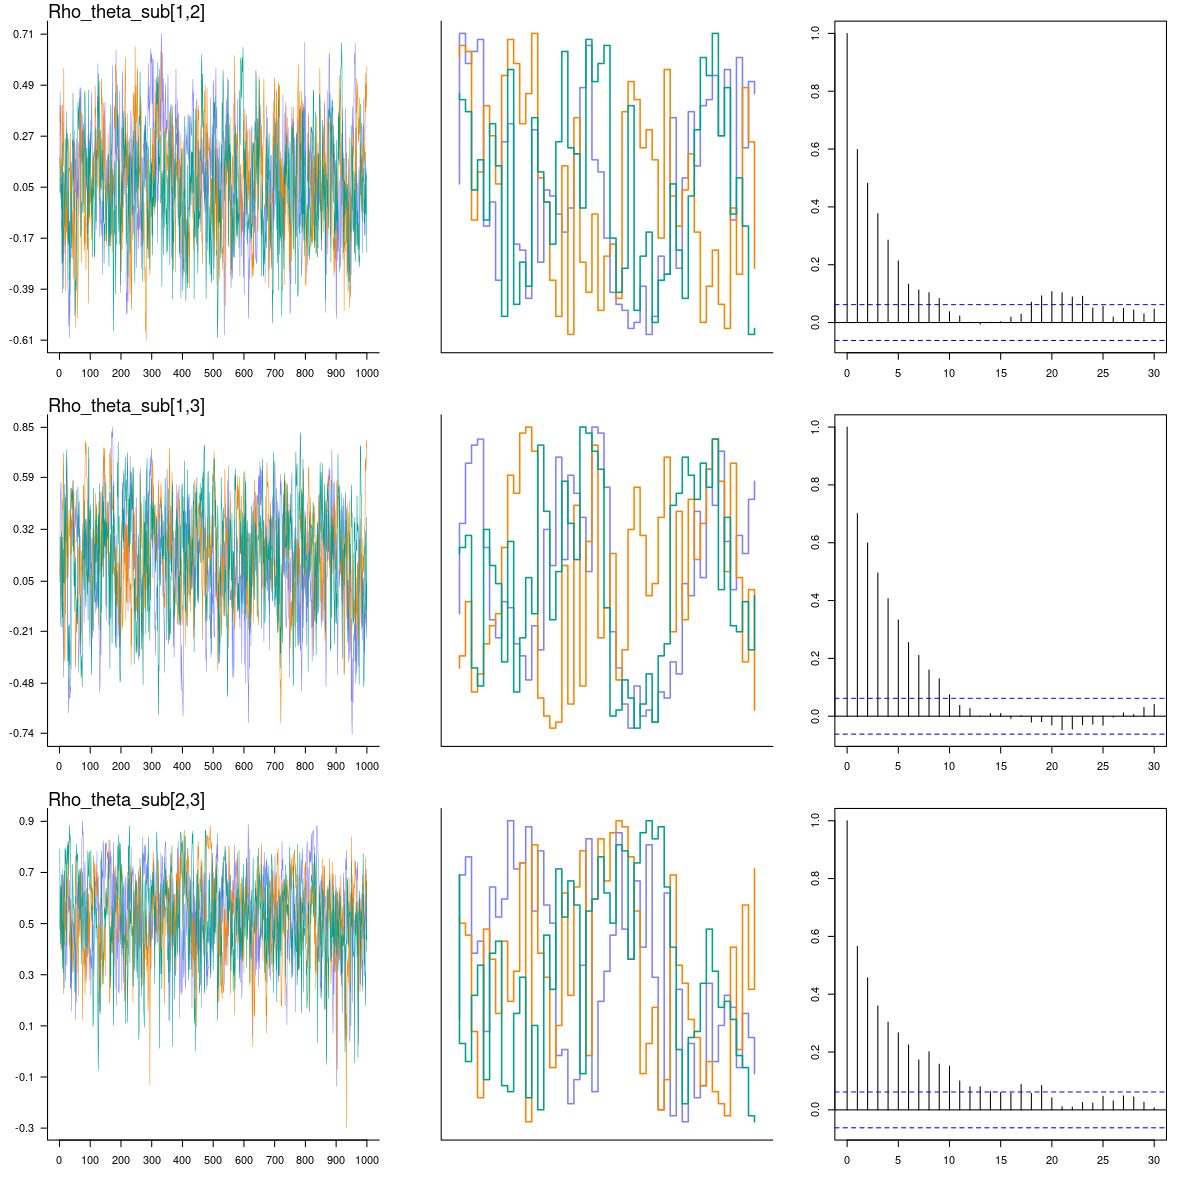
\includegraphics[width=1\linewidth]{FOLV_CE_J100_Ndata5_Rho}
	%
	\caption[First-order latent variable model (FOLV). Sample size $100$, replica number $5$. Centered parametrization. Correlation of sub-dimensions. Trace, trank and auto-correlation plots.]%
	{First-order latent variable model (FOLV). Sample size $100$, replica number $5$. Centered parametrization. Correlation of sub-dimensions: (Left) trace plot, (Middle) trank plot, (Right) auto-correlation plot.}
	\label{fig:FOLV_CE_chains8}
\end{figure}
%
\begin{figure}[H]
	\centering
	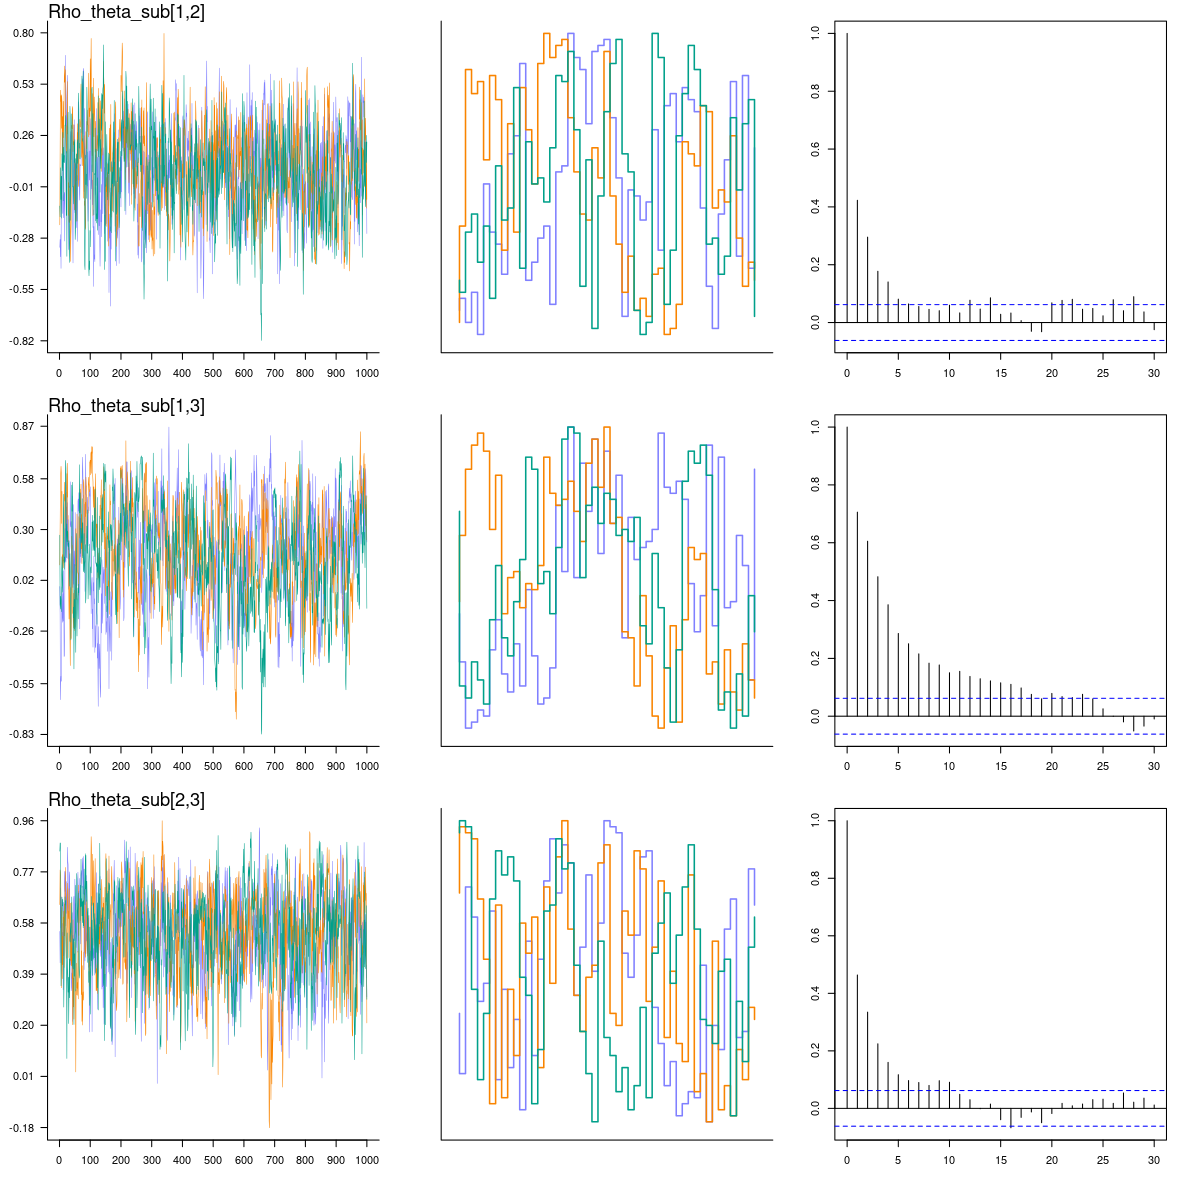
\includegraphics[width=1\linewidth]{FOLV_NC_J100_Ndata5_Rho}
	%
	\caption[First-order latent variable model (FOLV). Sample size $100$, replica number $5$. Non-centered parametrization. Correlation of sub-dimensions. Trace, trank and auto-correlation plots.]%
	{First-order latent variable model (FOLV). Sample size $100$, replica number $5$. Non-centered parametrization. Correlation of sub-dimensions: (Left) trace plot, (Middle) trank plot, (Right) auto-correlation plot.}
	\label{fig:FOLV_NC_chains8}
\end{figure}
%
\begin{figure}[H]
	\centering
	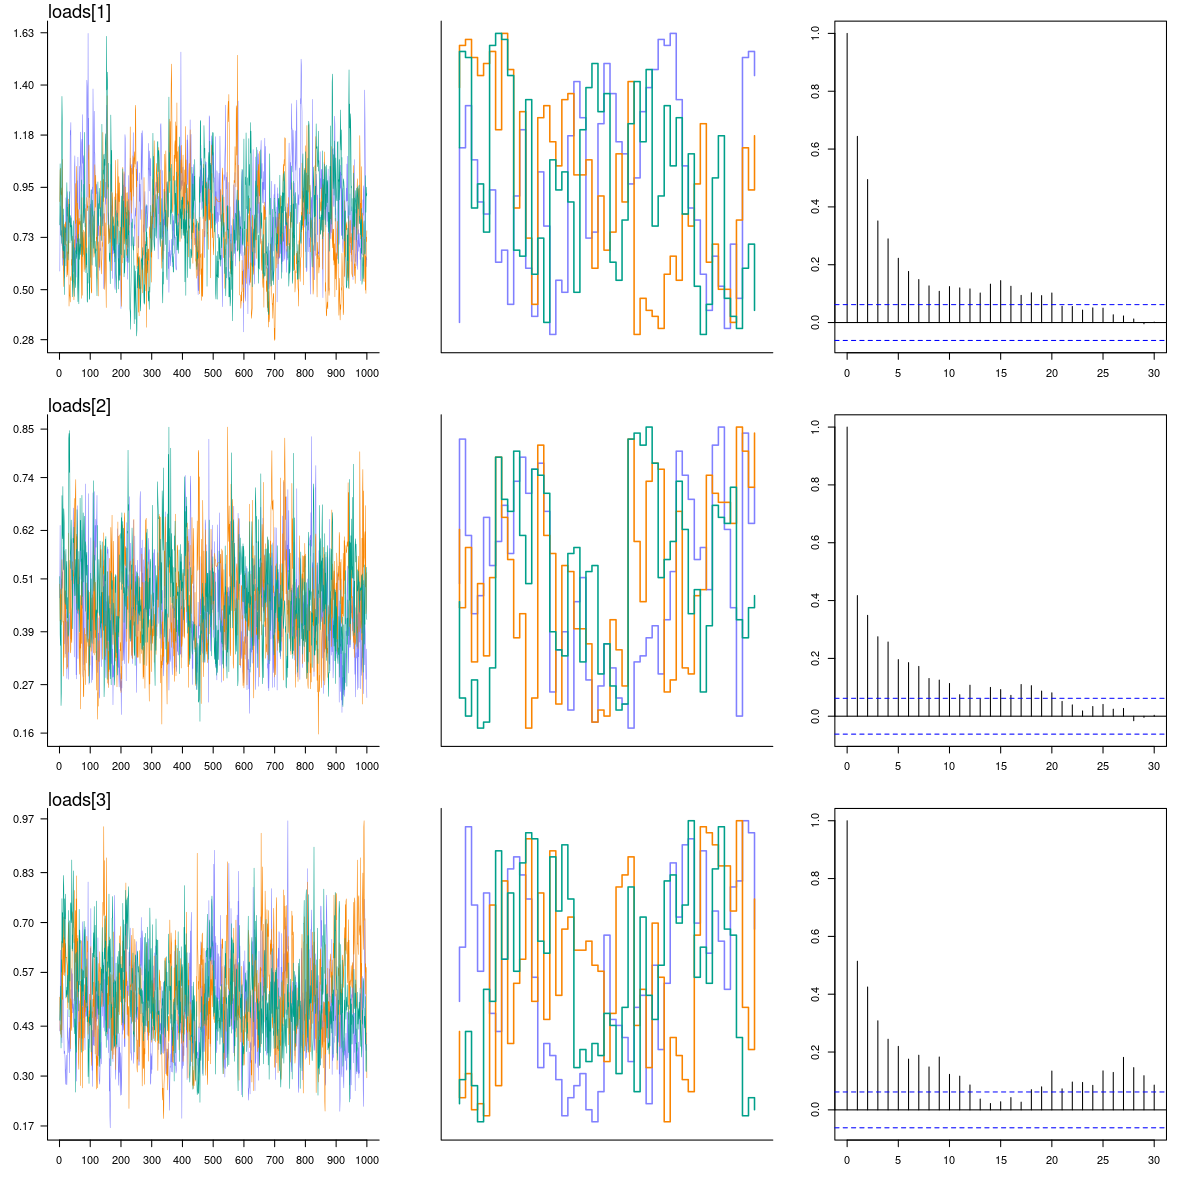
\includegraphics[width=1\linewidth]{SOLV_CE_J100_Ndata9_loads}
	%
	\caption[Second-order latent variable model (SOLV). Sample size $100$, replica number $9$. Centered parametrization. Loadings. Trace, trank and auto-correlation plots.]%
	{Second-order latent variable model (SOLV). Sample size $100$, replica number $9$. Centered parametrization. Loadings: (Left) trace plot, (Middle) trank plot, (Right) auto-correlation plot.}
	\label{fig:SOLV_CE_chains1}
\end{figure}
%
\begin{figure}[H]
	\centering
	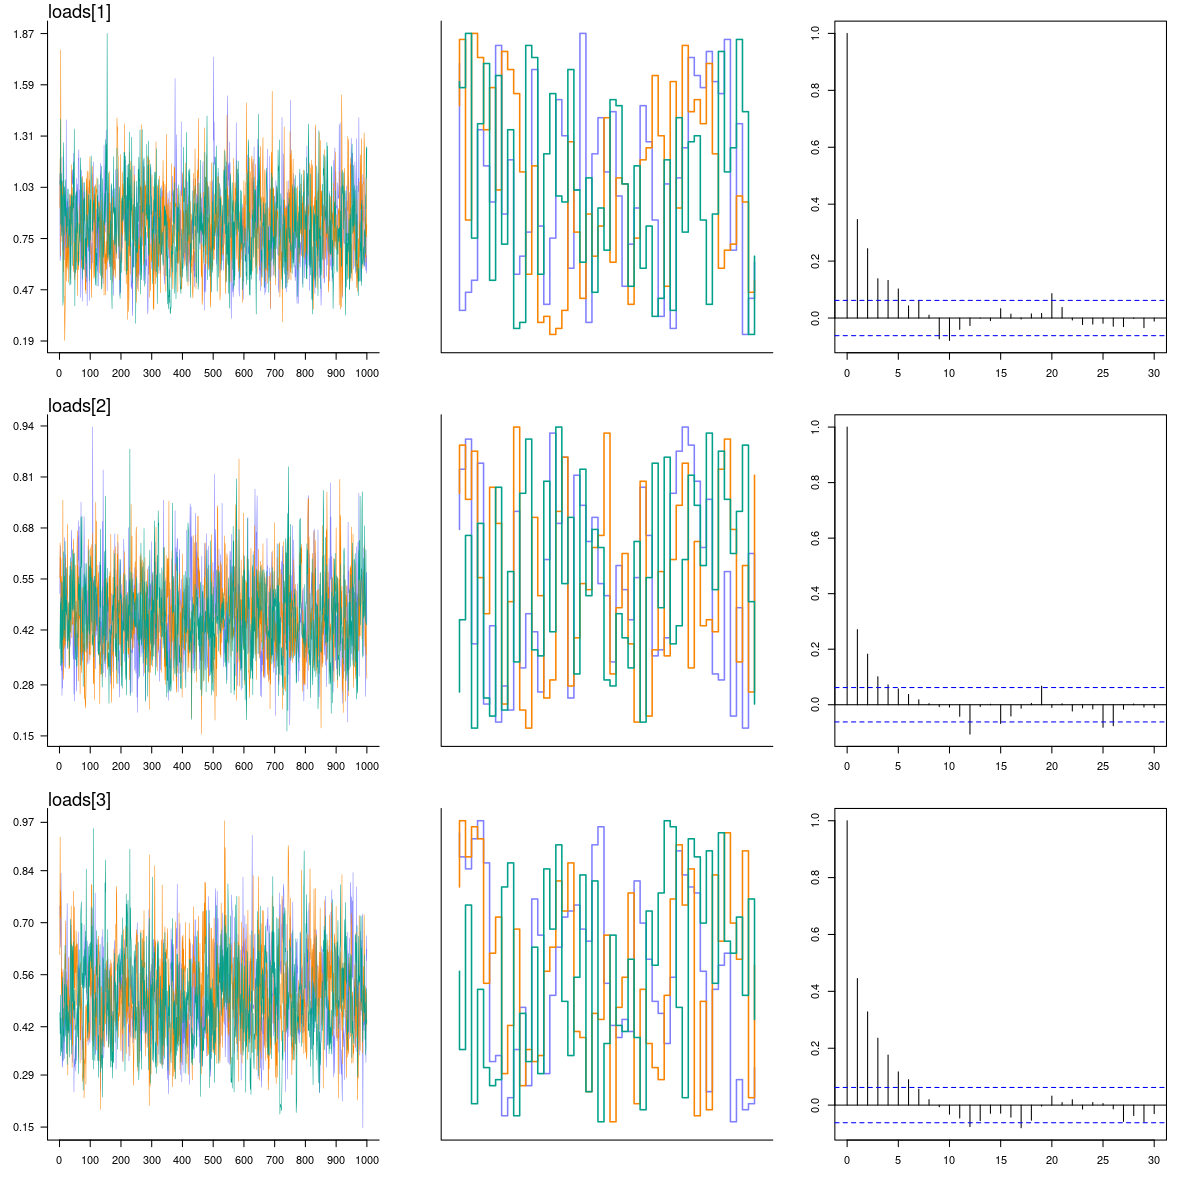
\includegraphics[width=1\linewidth]{SOLV_NC_J100_Ndata9_loads}
	%
	\caption[Second-order latent variable model (SOLV). Sample size $100$, replica number $9$. Non-centered parametrization. Loadings. Trace, trank and auto-correlation plots.]%
	{Second-order latent variable model (SOLV). Sample size $100$, replica number $9$. Non-centered parametrization. Loadings: (Left) trace plot, (Middle) trank plot, (Right) auto-correlation plot.}
	\label{fig:SOLV_NC_chains1}
\end{figure}
%
\begin{figure}[H]
	\centering
	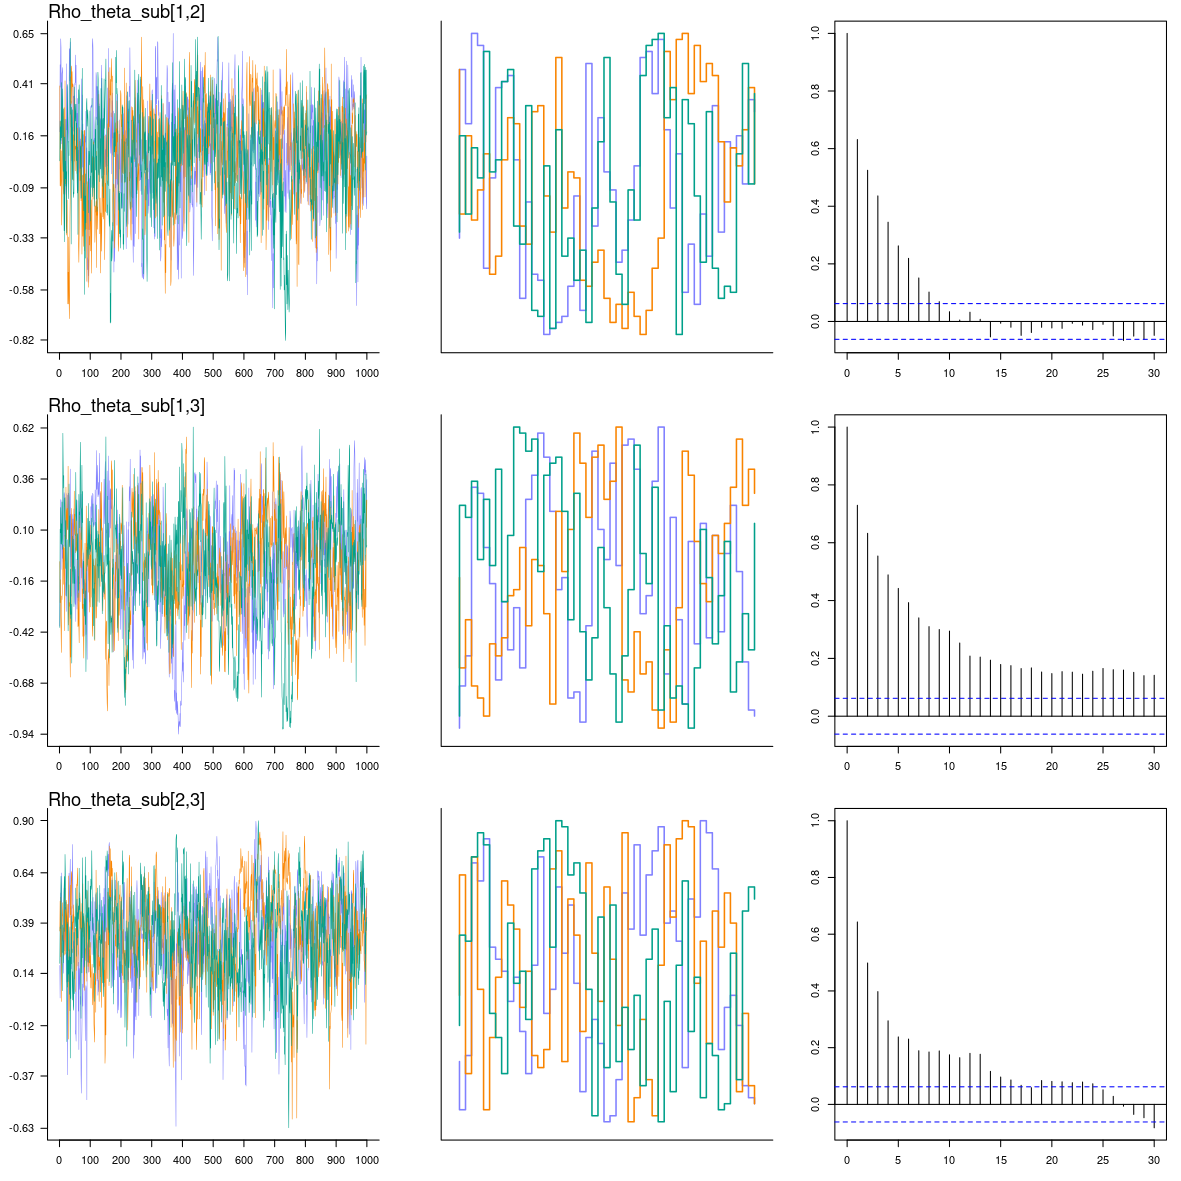
\includegraphics[width=1\linewidth]{SOLV_CE_J100_Ndata1_Rho}
	%
	\caption[Second-order latent variable model (SOLV). Sample size $100$, replica number $1$. Centered parametrization. Correlation of sub-dimensions. Trace, trank and auto-correlation plots.]%
	{Second-order latent variable model (SOLV). Sample size $100$, replica number $1$. Centered parametrization. Correlation of sub-dimensions: (Left) trace plot, (Middle) trank plot, (Right) auto-correlation plot.}
	\label{fig:SOLV_CE_chains2}
\end{figure}
%
\begin{figure}[H]
	\centering
	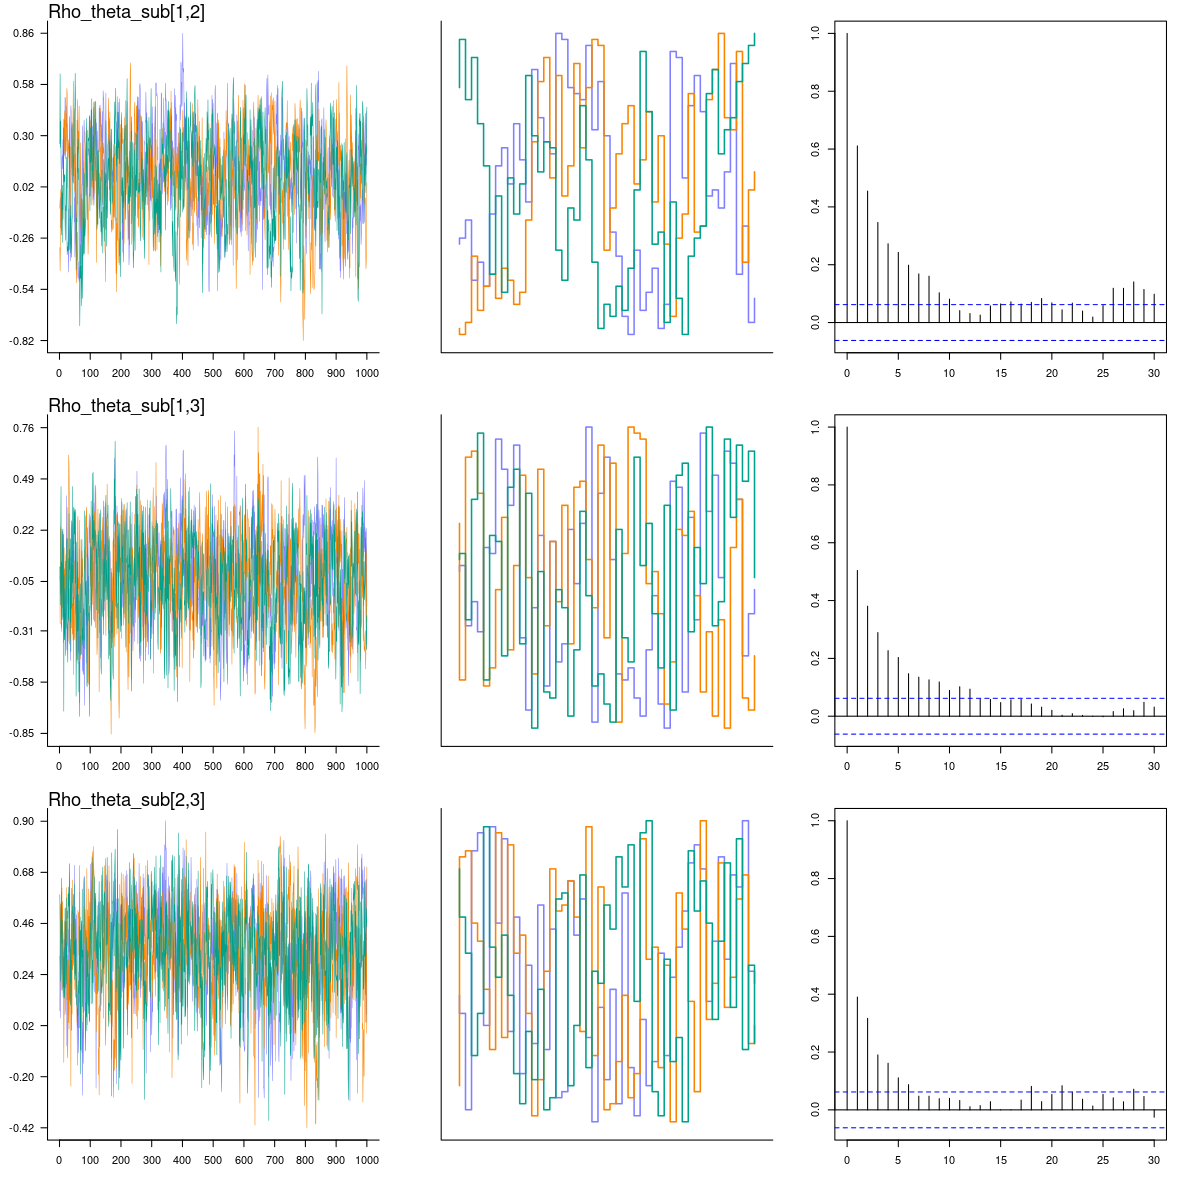
\includegraphics[width=1\linewidth]{SOLV_NC_J100_Ndata1_Rho}
	%
	\caption[Second-order latent variable model (SOLV). Sample size $100$, replica number $1$. Non-centered parametrization. Correlation of sub-dimensions. Trace, trank and auto-correlation plots.]%
	{Second-order latent variable model (SOLV). Sample size $100$, replica number $1$. Non-centered parametrization. Correlation of sub-dimensions: (Left) trace plot, (Middle) trank plot, (Right) auto-correlation plot.}
	\label{fig:SOLV_NC_chains2}
\end{figure}
%
\begin{figure}[H]
	\centering
	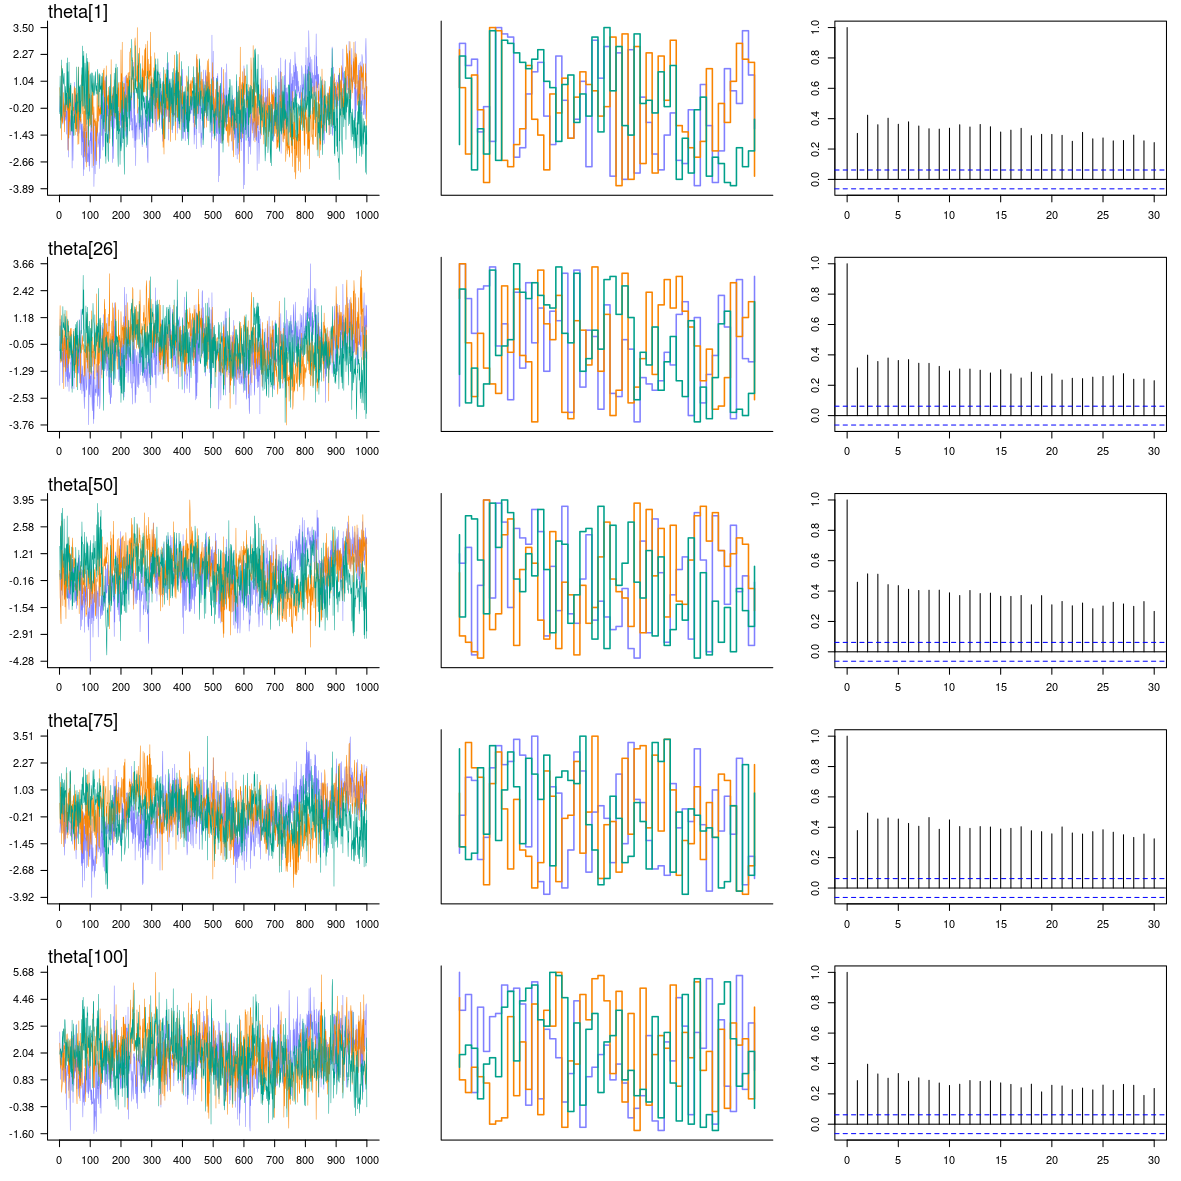
\includegraphics[width=1\linewidth]{SOLV_CE_J100_Ndata10_theta}
	%
	\caption[Second-order latent variable model (SOLV). Sample size $100$, replica number $10$. Centered parametrization. Highest-order dimension. Trace, trank and auto-correlation plots.]%
	{Second-order latent variable model (SOLV). Sample size $100$, replica number $10$. Centered parametrization. Highest-order dimension: (Left) trace plot, (Middle) trank plot, (Right) auto-correlation plot.}
	\label{fig:SOLV_CE_chains3}
\end{figure}
%
\begin{figure}[H]
	\centering
	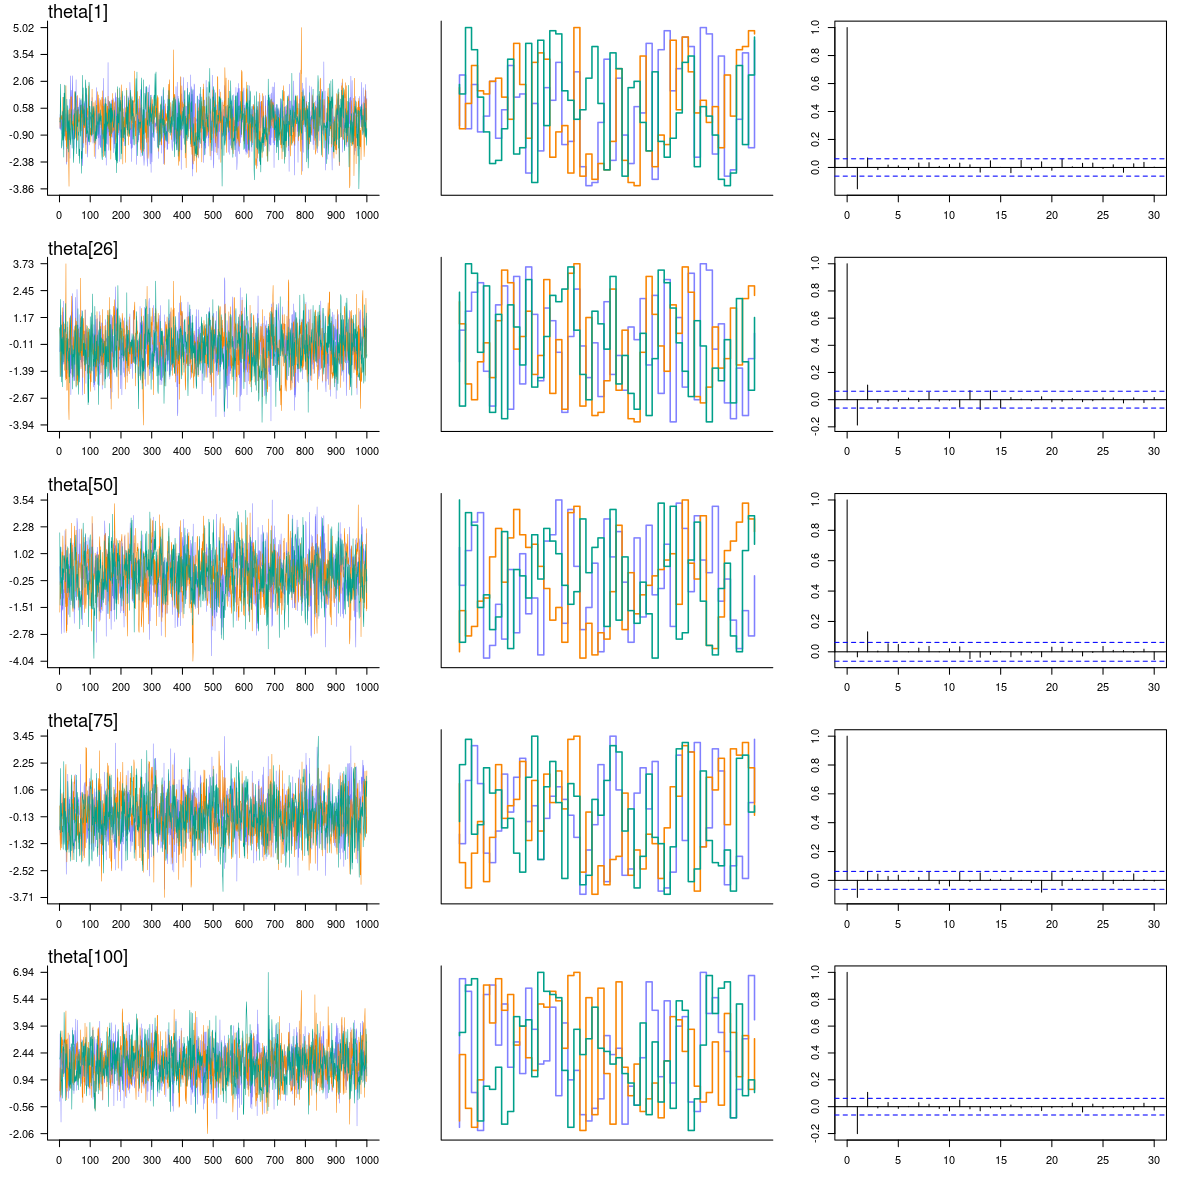
\includegraphics[width=1\linewidth]{SOLV_NC_J100_Ndata10_theta}
	%
	\caption[Second-order latent variable model (SOLV). Sample size $100$, replica number $10$. Non-centered parametrization. Highest-order dimension. Trace, trank and auto-correlation plots.]%
	{Second-order latent variable model (SOLV). Sample size $100$, replica number $10$. Non-centered parametrization. Highest-order dimension: (Left) trace plot, (Middle) trank plot, (Right) auto-correlation plot.}
	\label{fig:SOLV_NC_chains3}
\end{figure}
%
\begin{figure}[H]
	\centering
	\begin{subfigure}
		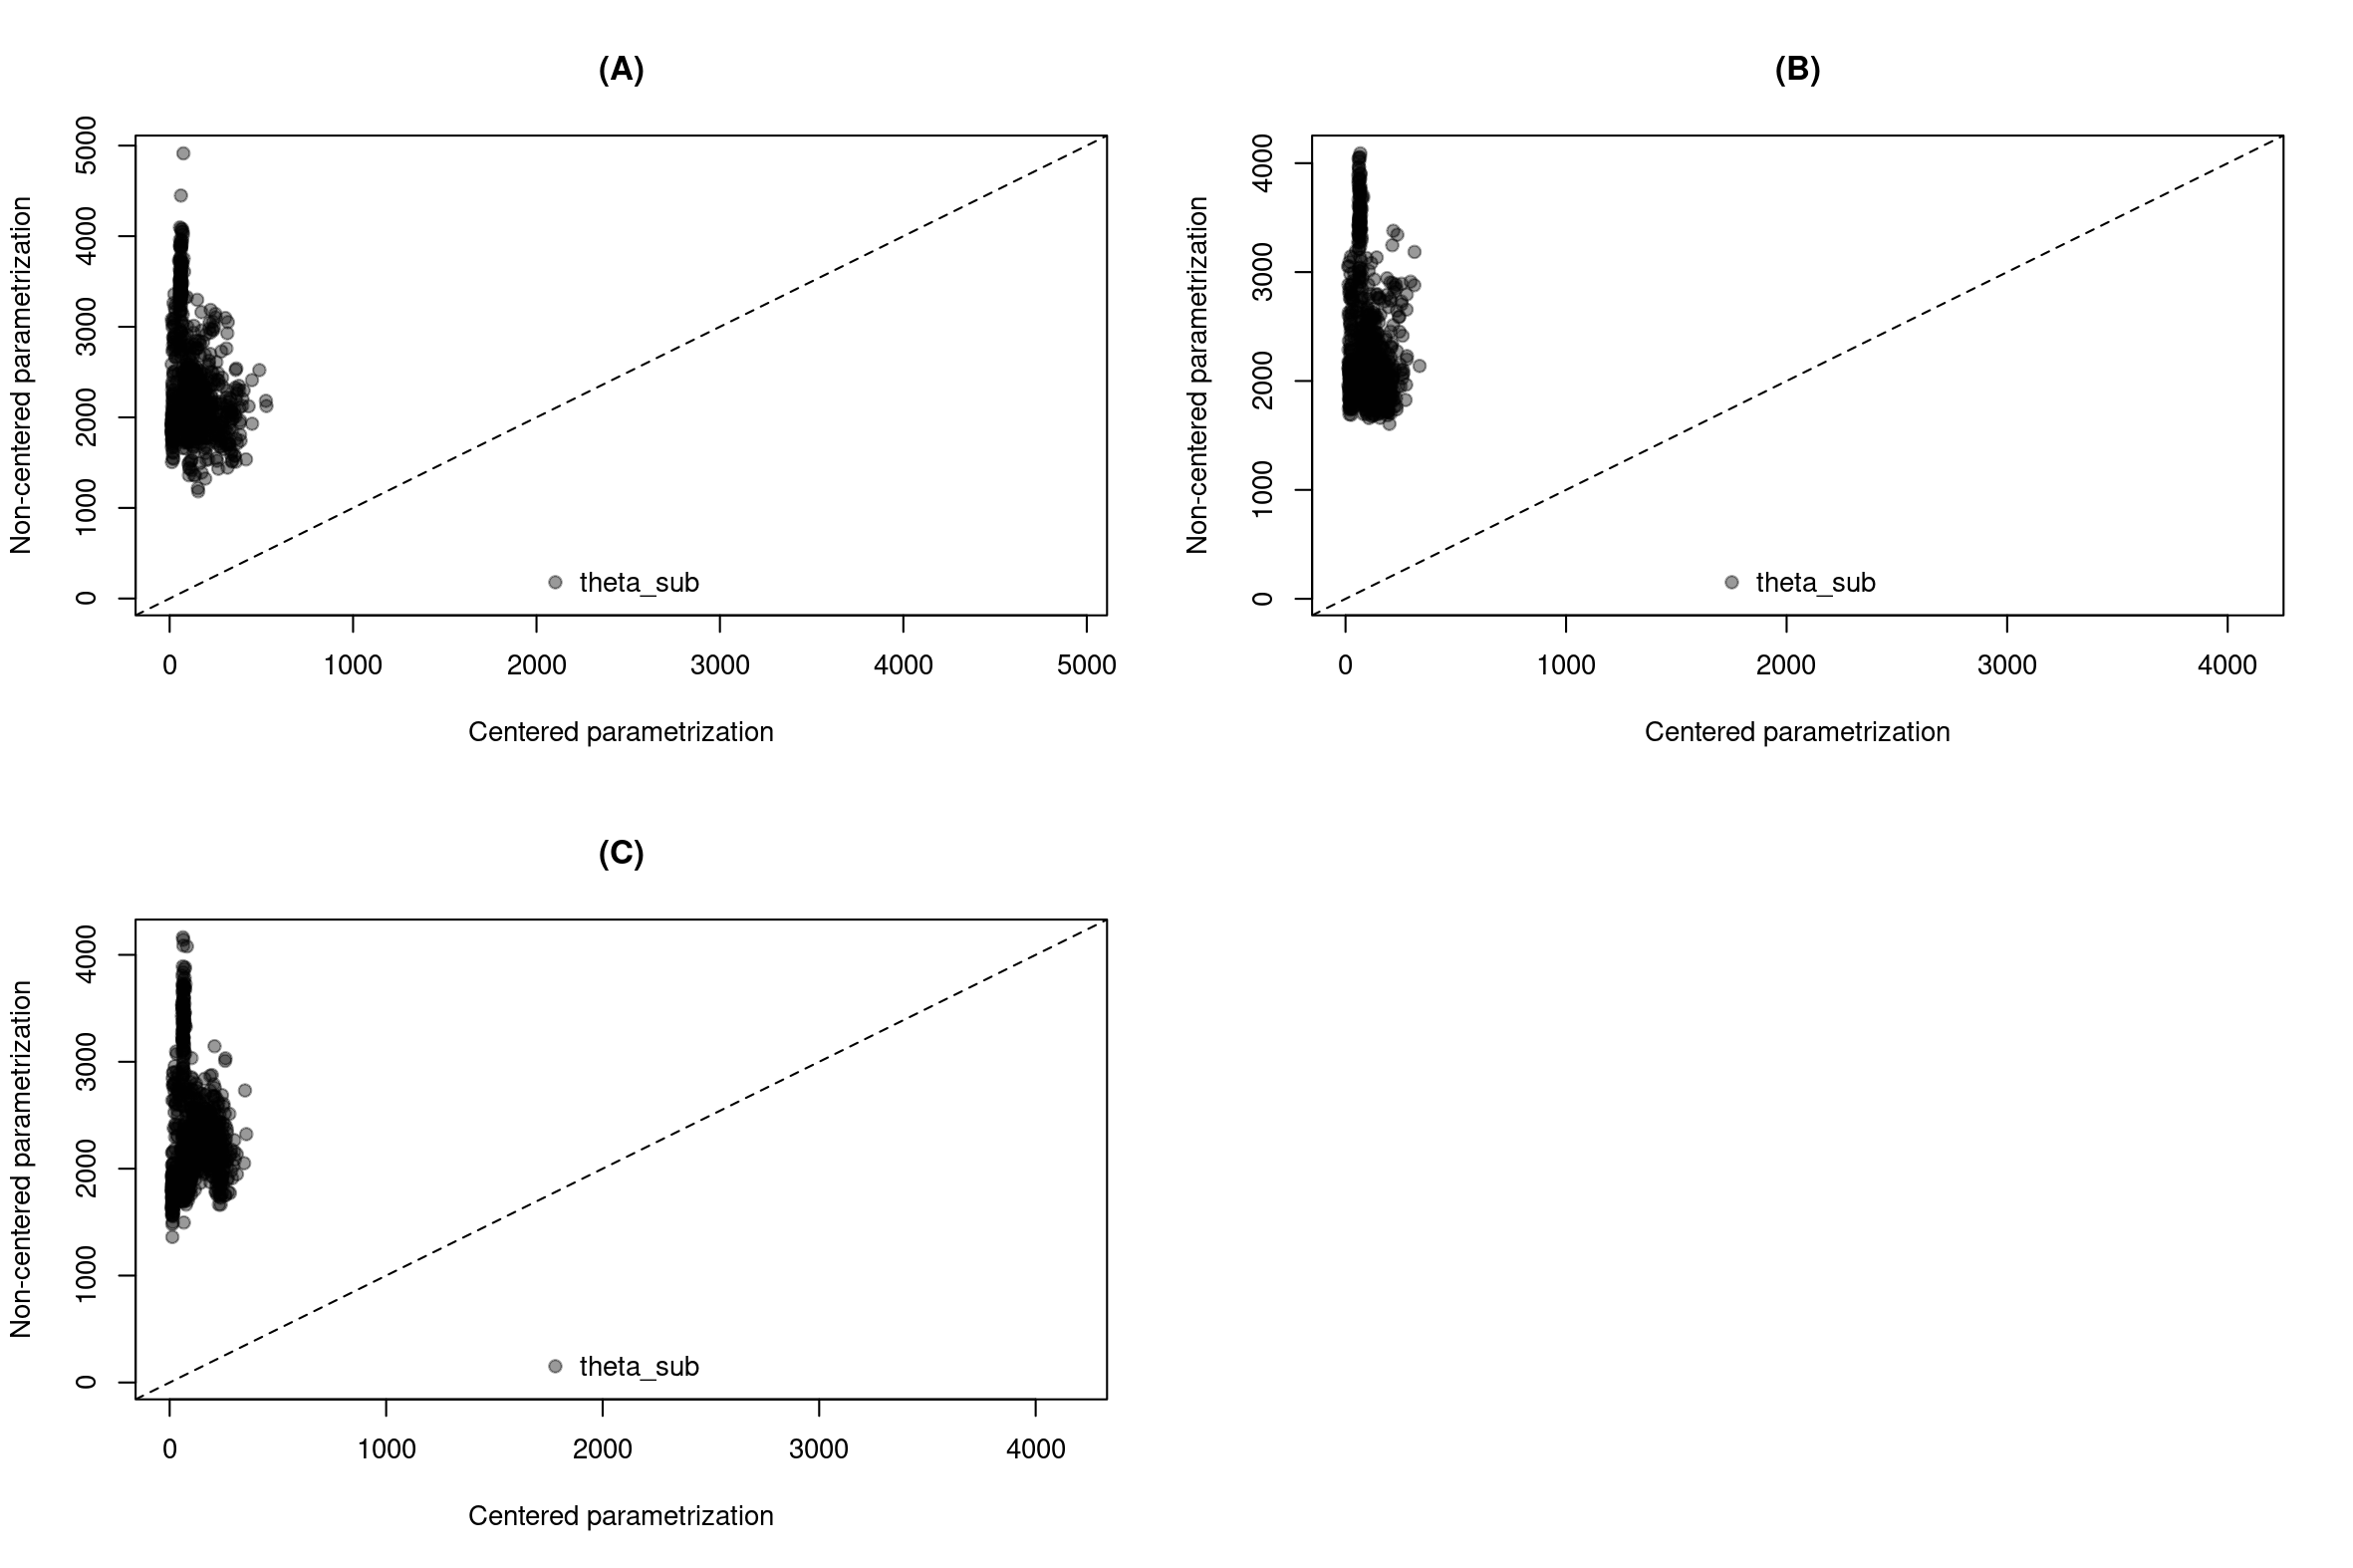
\includegraphics[width=1\linewidth]{FOLV_100_neff3}
	\end{subfigure}
	%
	\begin{subfigure}
		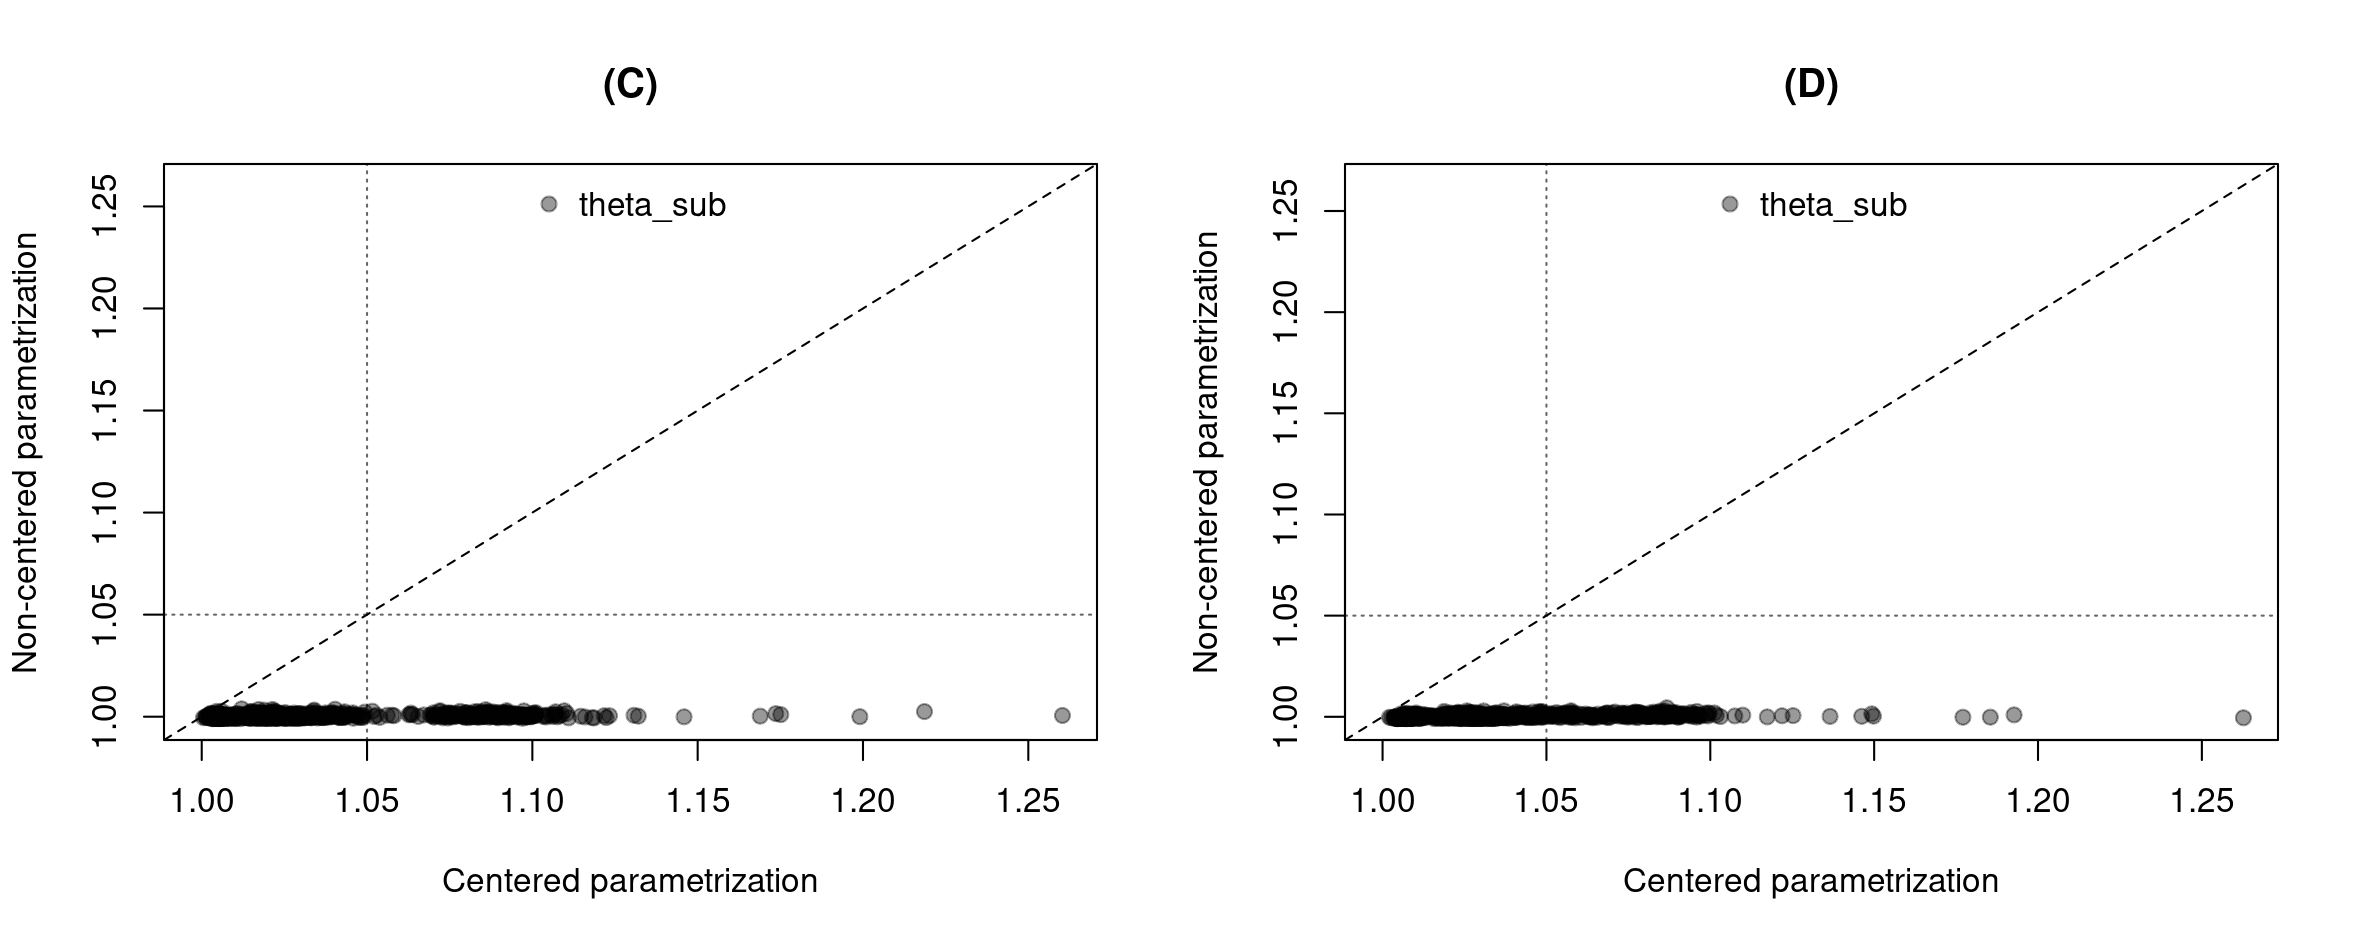
\includegraphics[width=1\linewidth]{FOLV_100_Rhat3}
	\end{subfigure}
	%
	\caption[First-order latent variable model (FOLV). Sample size $100$, all replicas. CP and NCP comparison plot.]%
	{First-order latent variable model (FOLV). Sample size $100$, all replicas. CP and NCP comparison plot. (A) \texttt{n\_eff} for the first sub-dimension. (B) \texttt{n\_eff} for the second sub-dimensions. (C) \texttt{Rhat} for the first sub-dimension. (D) \texttt{Rhat} for the second sub-dimensions. Diagonal discontinuous line describes equality between CP and NCP. Vertical and horizontal discontinuous lines is set at \texttt{Rhat}$=1.05$. }
	\label{fig:FOLV_stat3}
\end{figure}
%
\begin{figure}[H]
	\centering
	\begin{subfigure}
		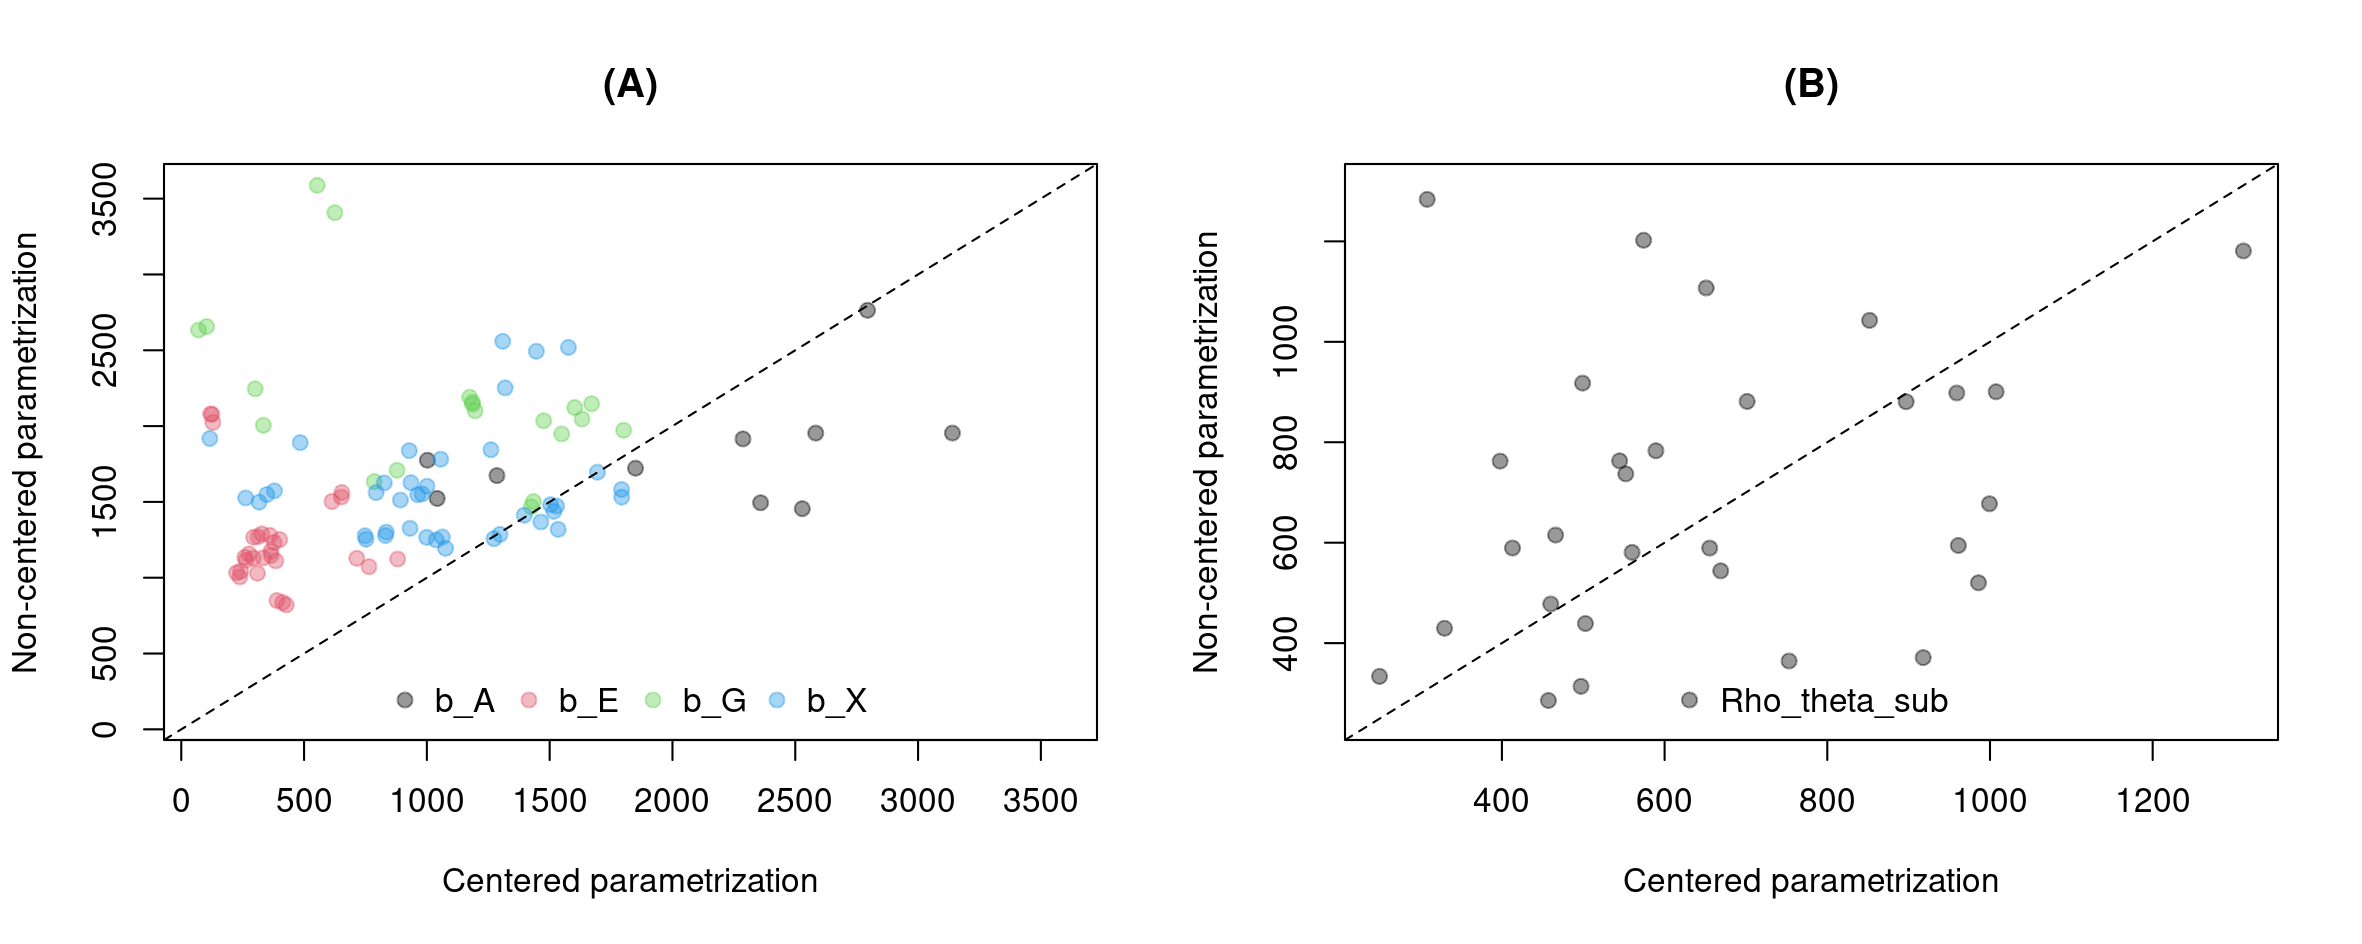
\includegraphics[width=1\linewidth]{FOLV_100_neff2}
	\end{subfigure}
	%
	\begin{subfigure}
		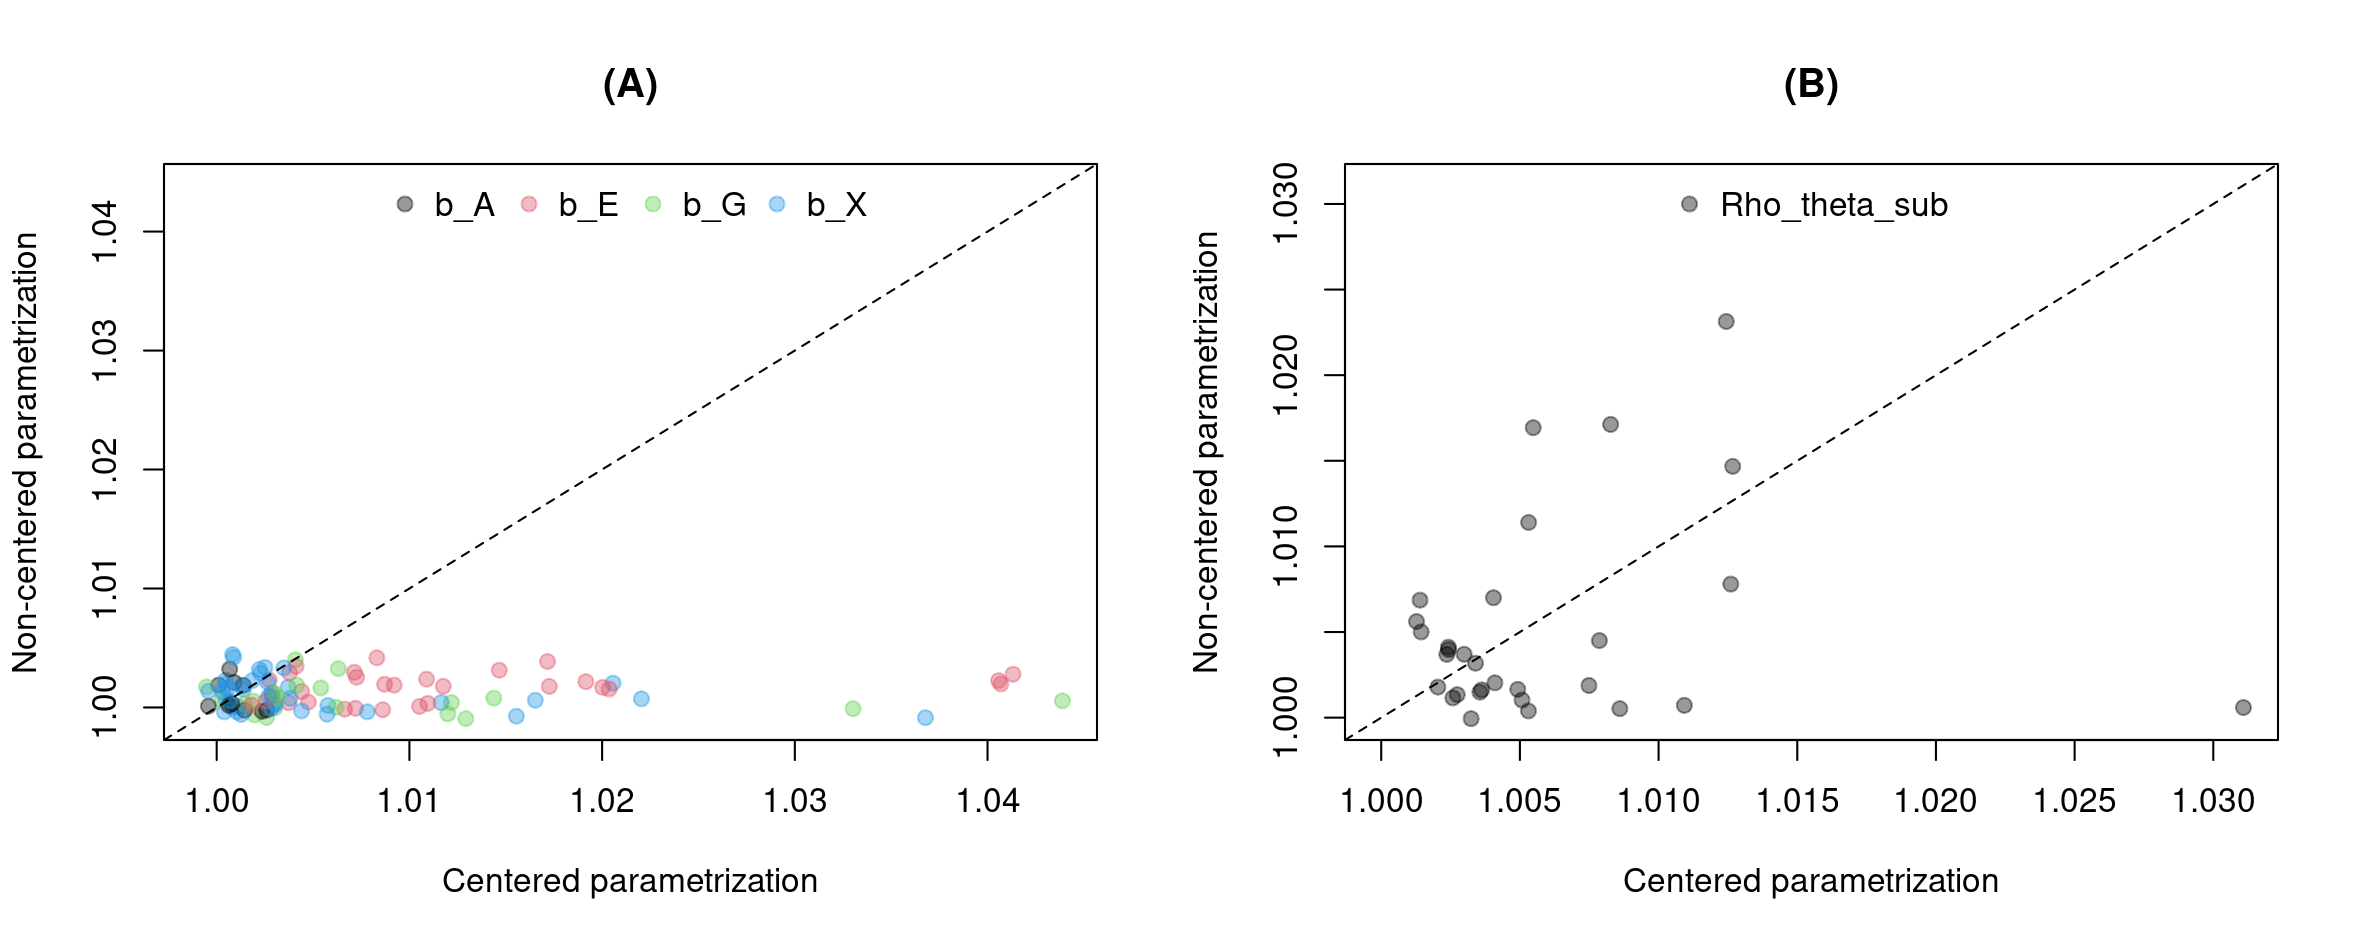
\includegraphics[width=1\linewidth]{FOLV_100_Rhat2}
	\end{subfigure}
	%
	\caption[First-order latent variable model (FOLV). Sample size $100$, all replicas. CP and NCP comparison plot.]%
	{First-order latent variable model (FOLV). Sample size $100$, all replicas. CP and NCP comparison plot. (A) \texttt{n\_eff} for regression parameters. (B) \texttt{n\_eff} for correlations among sub-dimensions. (C) \texttt{Rhat} for regression parameters. (D) \texttt{Rhat} for correlations among sub-dimensions. Diagonal discontinuous line describes equality between CP and NCP. Vertical and horizontal discontinuous lines is set at \texttt{Rhat}$=1.05$. }
	\label{fig:FOLV_stat2}
\end{figure}
%
\begin{figure}[H]
	\centering
	\begin{subfigure}
		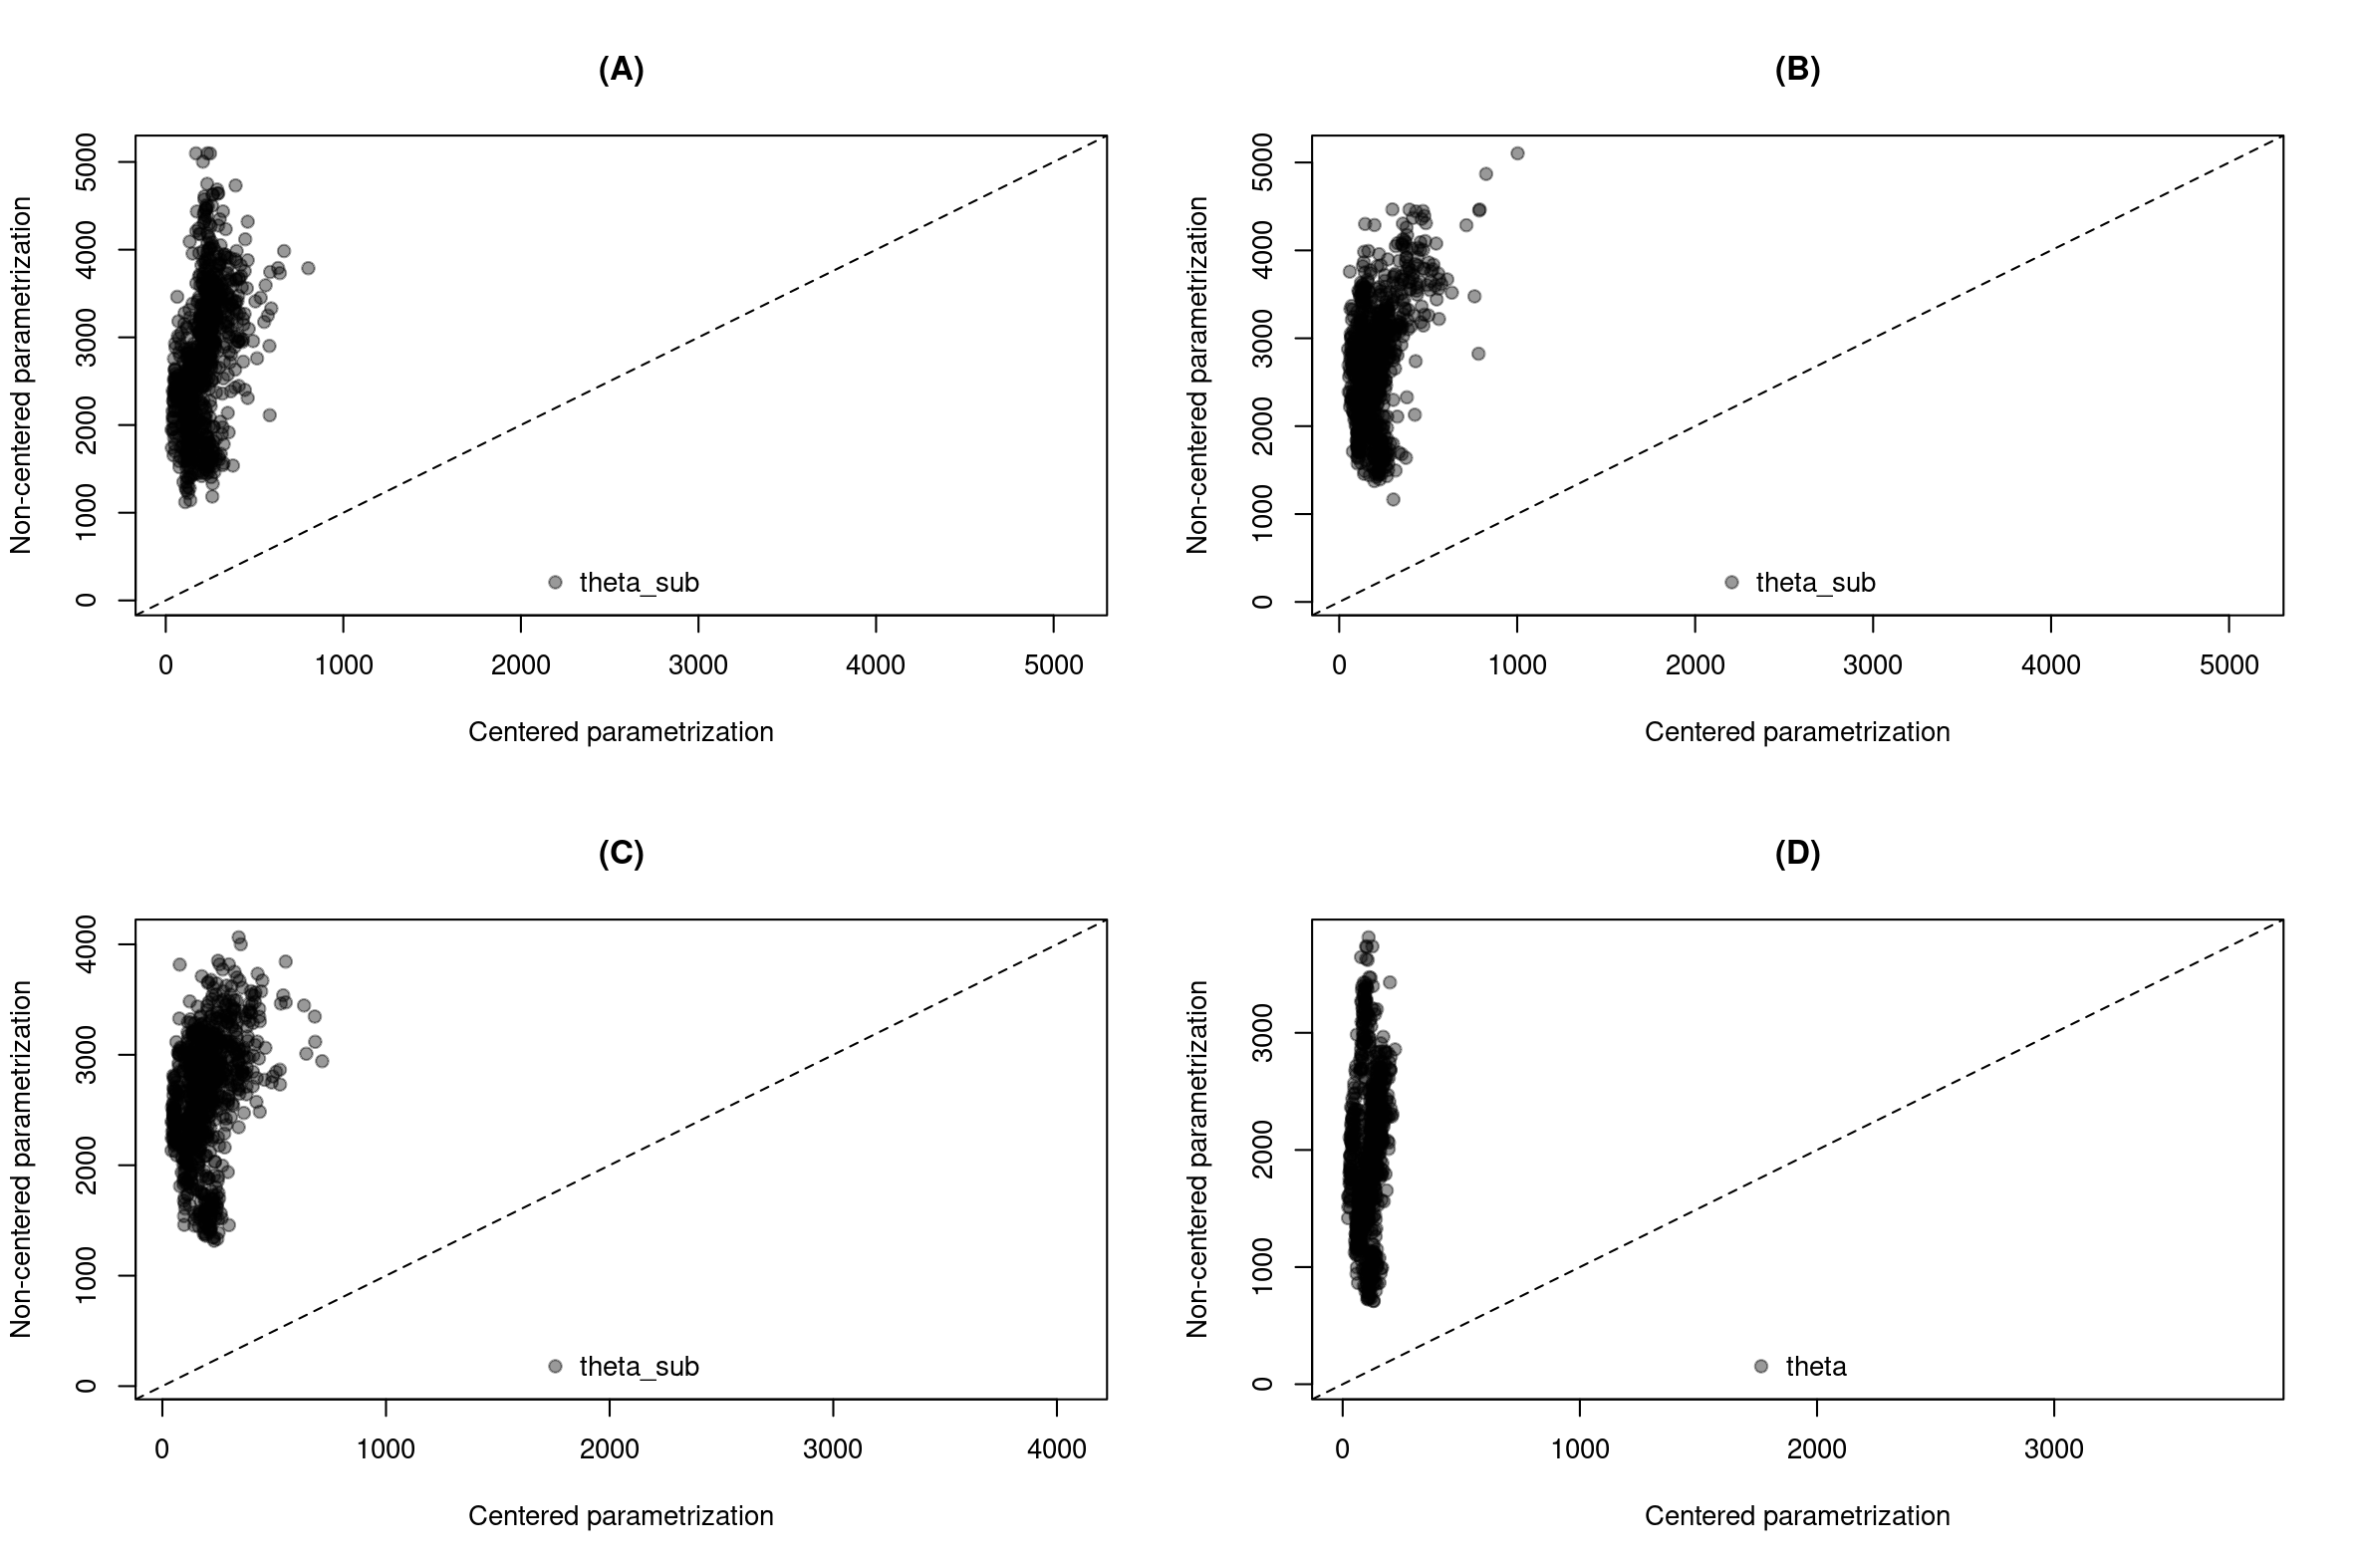
\includegraphics[width=1\linewidth]{SOLV_100_neff3}
	\end{subfigure}
	%
	\begin{subfigure}
		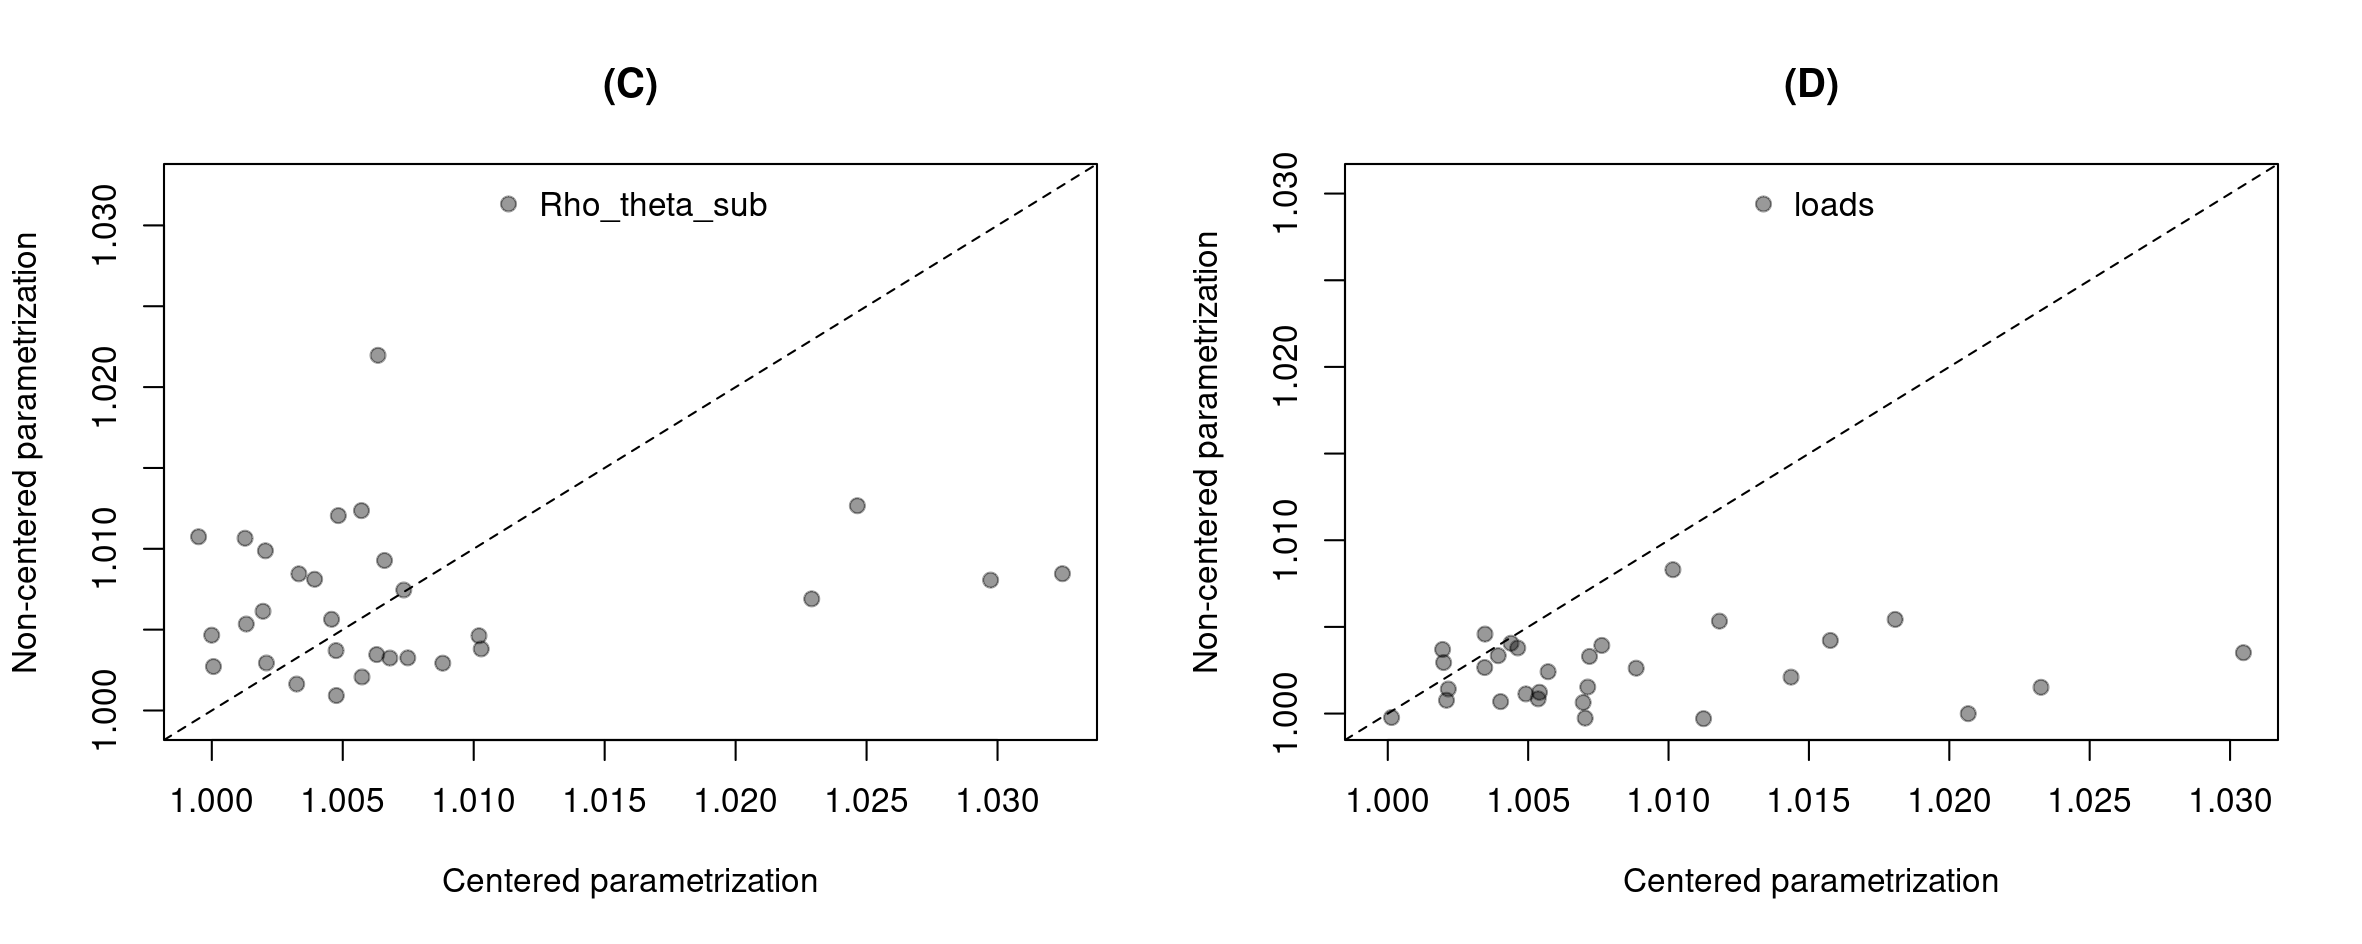
\includegraphics[width=1\linewidth]{SOLV_100_Rhat3}
	\end{subfigure}
	%
	\caption[Second-order latent variable model (SOLV). Sample size $100$, all replicas. CP and NCP comparison plot.]%
	{Second-order latent variable model (SOLV). Sample size $100$, all replicas. CP and NCP comparison plot. (A) \texttt{n\_eff} for the correlations among sub-dimension. (B) \texttt{n\_eff} for the loadings. (C) \texttt{Rhat} for the correlation among sub-dimensions. (D) \texttt{Rhat} for the loadings. Diagonal discontinuous line describes equality between CP and NCP. Vertical and horizontal discontinuous lines is set at \texttt{Rhat}$=1.05$. }
	\label{fig:SOLV_stat1}
\end{figure}
%
\begin{figure}[H]
	\centering
	\begin{subfigure}
		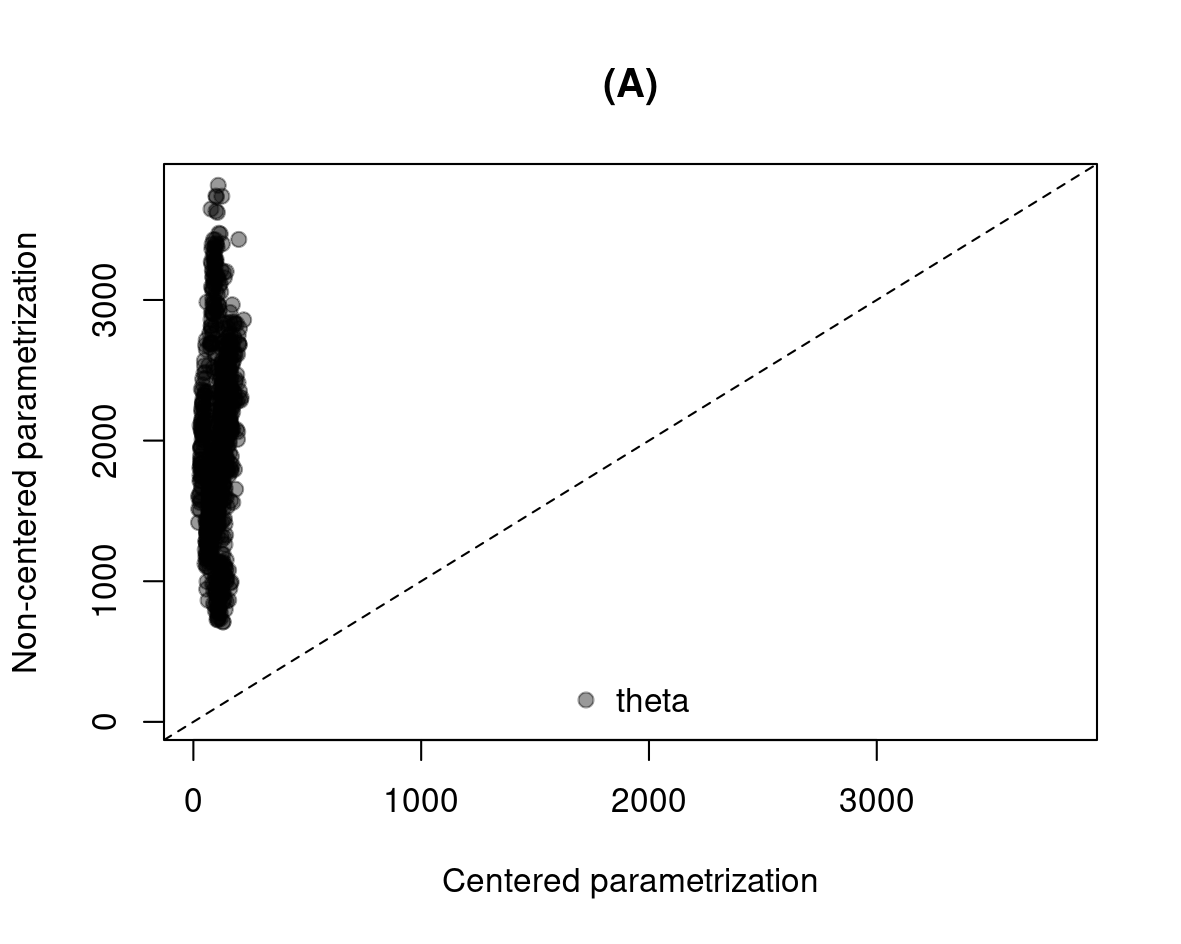
\includegraphics[width=0.48\linewidth]{SOLV_100_neff6}
	\end{subfigure}
	%
	\begin{subfigure}
		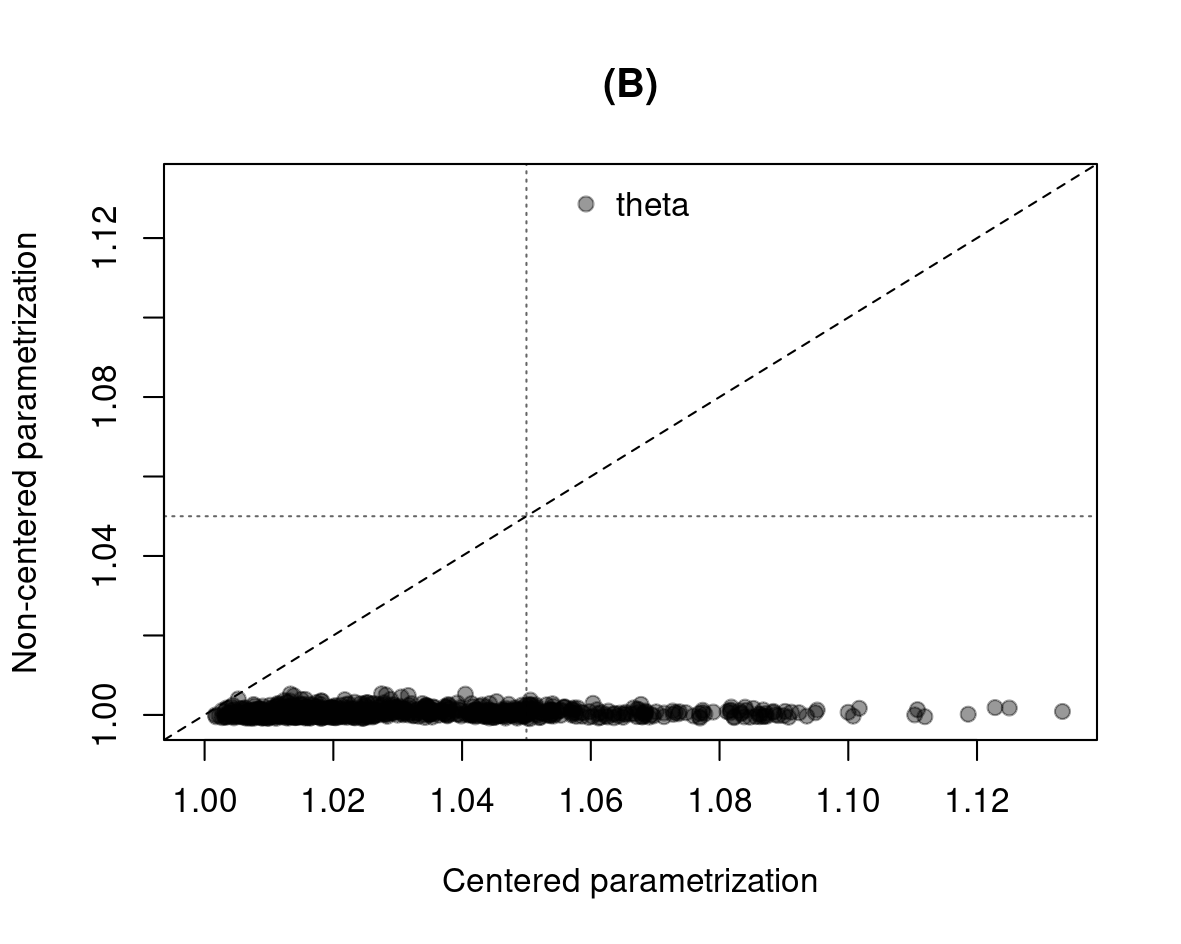
\includegraphics[width=0.48\linewidth]{SOLV_100_Rhat6}
	\end{subfigure}
	%
	\caption[Second-order latent variable model (SOLV). Sample size $100$, all replicas. CP and NCP comparison plot.]%
	{Second-order latent variable model (SOLV). Sample size $100$, all replicas. CP and NCP comparison plot. (A) \texttt{n\_eff} for the higher-order latent variable. (B) \texttt{Rhat} for the higher-order latent variable. Diagonal discontinuous line describes equality between CP and NCP. Vertical and horizontal discontinuous lines is set at \texttt{Rhat}$=1.05$. }
	\label{fig:SOLV_stat2}
\end{figure}
%
\begin{figure}[H]
	\centering
	\begin{subfigure}
		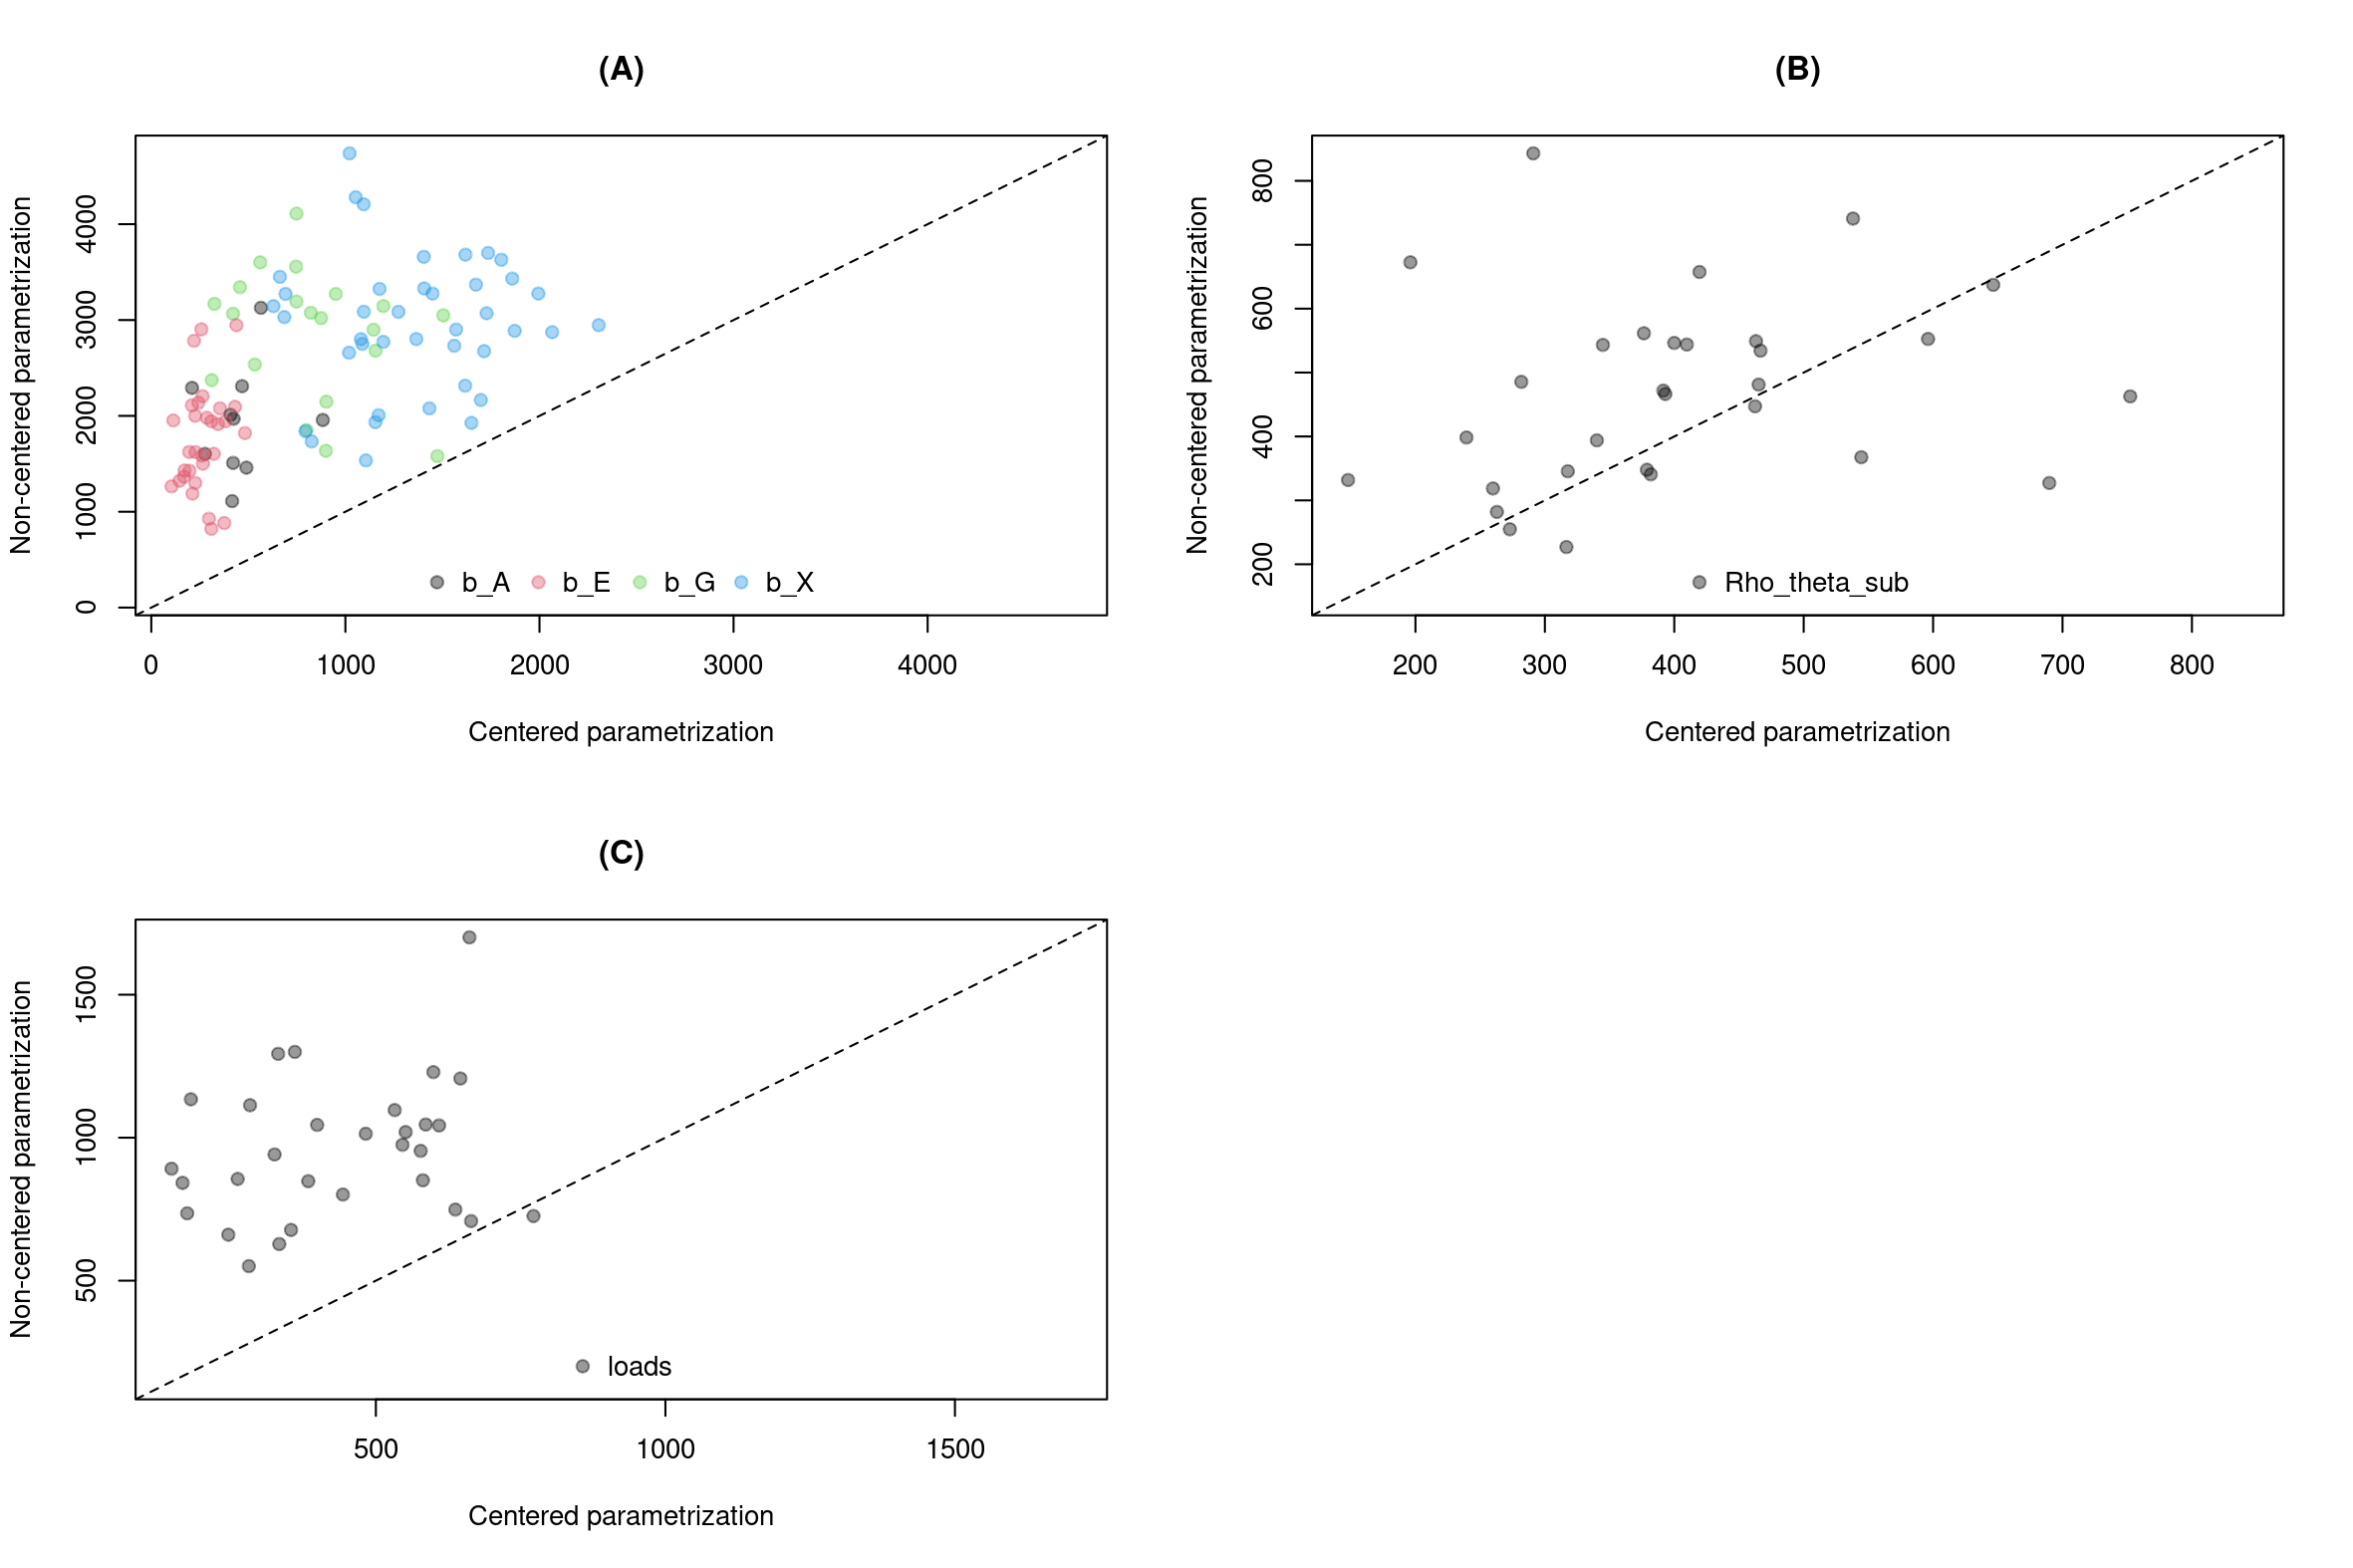
\includegraphics[width=0.48\linewidth]{SOLV_100_neff2}
	\end{subfigure}
	%
	\begin{subfigure}
		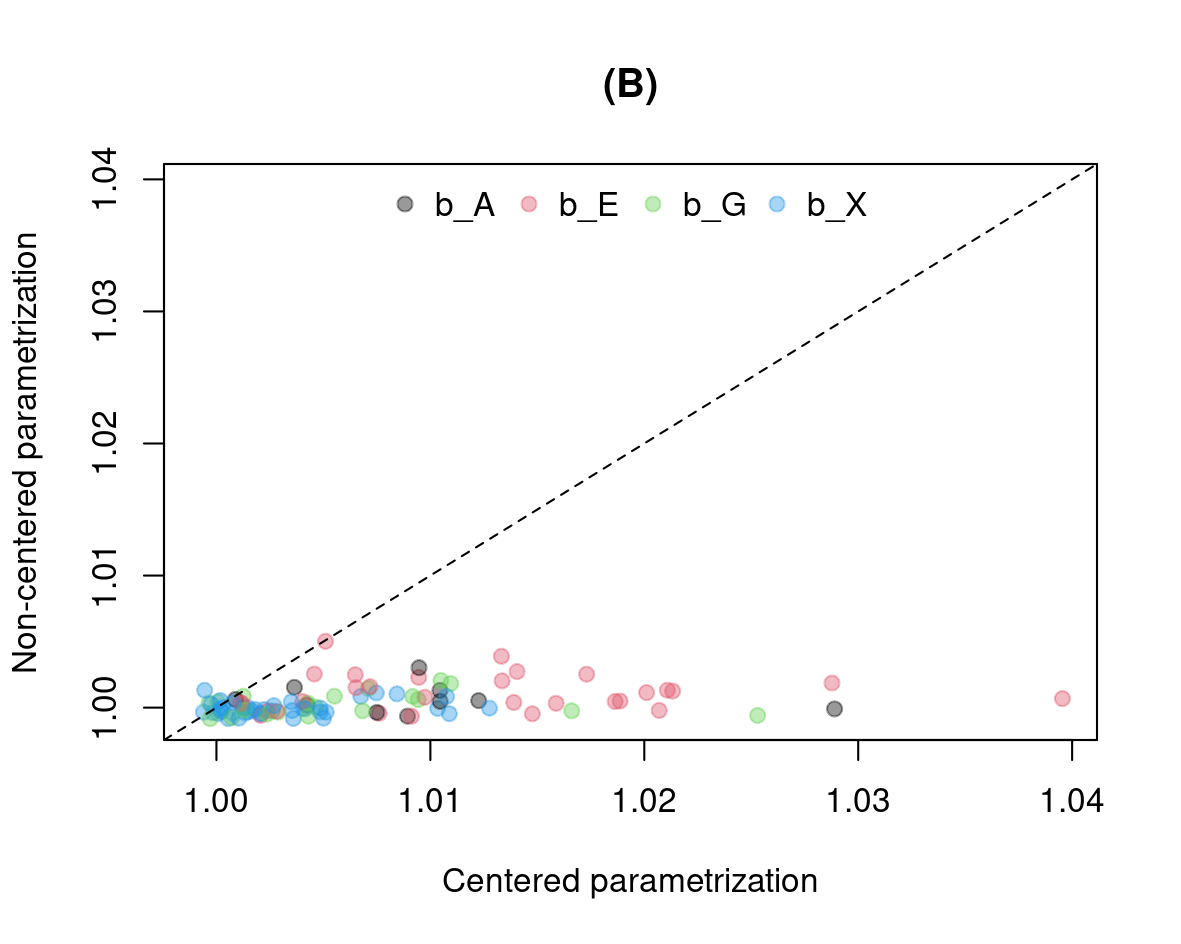
\includegraphics[width=0.48\linewidth]{SOLV_100_Rhat2}
	\end{subfigure}
	%
	\caption[Second-order latent variable model (SOLV). Sample size $100$, all replicas. CP and NCP comparison plot.]%
	{Second-order latent variable model (SOLV). Sample size $100$, all replicas. CP and NCP comparison plot. (A) \texttt{n\_eff} for regression parameters. (B) \texttt{Rhat} for the first sub-dimension. (C) \texttt{Rhat} for regression parameters. (D) \texttt{Rhat} for the second sub-dimensions. Diagonal discontinuous line describes equality between CP and NCP. Vertical and horizontal discontinuous lines is set at \texttt{Rhat}$=1.05$. }
	\label{fig:SOLV_stat3}
\end{figure}



%%%%%%%%%%%%%%%%%%%%%%%%%%%%%%%%%%%%%%%%%%%%%%%%%%%%%%%%%%%%%%%%%%%%%%%
\newpage
\subsection{Recovery capacity} \label{sub_sect:recovery}

This section shows only a small set of tables about the recovery capacity of the model. In case the reader wants to replicate the calculations or access the full set of statistics refer to the ``data/tables" section of the accompanying github page:

\noindent \url{https://github.com/jriveraespejo/thesis/tree/master/data_tables} \\

Moreover, in case the reader wants to inspect the recovery plots per model, parametrization, sample size, and replica refer to the ``recovery plots" image section of the accompanying github page:

\noindent \url{https://github.com/jriveraespejo/thesis/tree/master/images/recovery_plots} \\
%
\begin{table}[H]
	\centering
	\begin{tabular}{rlrrrrr}
		\hline
		\multicolumn{2}{c}{ } & Number of & \multicolumn{4}{c}{ RMSE $( \theta^{(2)}_{j1} )$ } \\ 
		\cmidrule(rl){4-7}
		& Parametrization & individuals(replicas) & mean & sd & min & max \\  
		\hline\hline
		1 & CP &  100(10) & 0.639 & 0.151 & 0.223 & 1.069 \\ 
		2 & CP &  250(10) & 0.594 & 0.138 & 0.254 & 1.103 \\ 
		3 & CP &  500(10) & 0.623 & 0.145 & 0.215 & 1.079 \\ 
		%
		\hline
		%
		4 & NCP &  100(10) & 0.632 & 0.148 & 0.256 & 1.032 \\  
		5 & NCP &  250(10) & 0.589 & 0.136 & 0.271 & 1.066 \\ 
		6 & NCP &  500(10) & 0.610 & 0.143 & 0.214 & 1.087 \\  
		\hline
	\end{tabular}
	\caption[First-order latent variable model (FOLV). Aggregated RMSE for the first individual sub-dimension.]%
	{First-order latent variable model (FOLV). Aggregated RMSE for the first individual sub-dimension.}
	\label{tab:FOLV_RMSE_theta1}
\end{table}
%
\begin{table}[H]
	\centering
	\begin{tabular}{rlrrrrr}
		\hline
		\multicolumn{2}{c}{ } & Number of & \multicolumn{4}{c}{ RMSE $( \theta^{(2)}_{j2} )$} \\ 
		\cmidrule(rl){4-7}
		& Parametrization & individuals(replicas) & mean & sd & min & max \\  
		\hline\hline
		1 & CP &  100(10) & 0.608 & 0.148 & 0.318 & 0.930 \\ 
		2 & CP &  250(10) & 0.599 & 0.134 & 0.256 & 0.939 \\  
		3 & CP &  500(10) & 0.618 & 0.143 & 0.228 & 1.056 \\  
		%
		\hline
		%
		4 & NCP &  100(10) & 0.601 & 0.145 & 0.295 & 0.911 \\ 
		5 & NCP &  250(10) & 0.593 & 0.135 & 0.253 & 0.963 \\ 
		6 & NCP &  500(10) & 0.607 & 0.138 & 0.202 & 1.055 \\
		\hline
	\end{tabular}
	\caption[First-order latent variable model (FOLV). Aggregated RMSE for the second individual sub-dimension.]%
	{First-order latent variable model (FOLV). Aggregated RMSE for the second individual sub-dimension.}
	\label{tab:FOLV_RMSE_theta2}
\end{table}
%
\begin{table}[H]
	\centering
	\begin{tabular}{rlrrrrr}
		\hline
		\multicolumn{2}{c}{ } & Number of & \multicolumn{4}{c}{ RMSE $( \theta^{(2)}_{j3} )$} \\ 
		\cmidrule(rl){4-7}
		& Parametrization & individuals(replicas) & mean & sd & min & max \\  
		\hline\hline
		1 & CP &  100 & 0.604 & 0.142 & 0.257 & 1.000 \\  
		2 & CP &  250 & 0.612 & 0.128 & 0.321 & 0.973 \\  
		3 & CP &  500 & 0.612 & 0.150 & 0.172 & 1.079 \\ 
		%
		\hline
		%
		4 & NCP &  100 & 0.595 & 0.139 & 0.245 & 0.968 \\  
		5 & NCP &  250 & 0.609 & 0.131 & 0.288 & 0.990 \\ 
		6 & NCP &  500 & 0.601 & 0.147 & 0.220 & 1.082 \\  
		\hline
	\end{tabular}
	\caption[First-order latent variable model (FOLV). Aggregated RMSE for the third individual sub-dimension.]%
	{First-order latent variable model (FOLV). Aggregated RMSE for the third individual sub-dimension.}
	\label{tab:FOLV_RMSE_theta3}
\end{table}
%
\begin{table}[H]
	\centering
	\begin{tabular}{rlllrrrr}		
		\hline
		\multicolumn{4}{c}{ } & Number of &\multicolumn{3}{c}{ Sample size } \\ 
		\cmidrule(rl){6-8}
		& Parametrization & Variable & Parameter & replicas & 100 & 250 & 500 \\ 
		\hline\hline
		1 & CP & \footnotesize{Intercept} & $\Gamma_{0}$ &   10 & 0.097 & 0.070 & 0.082 \\ 
		2 & CP & \footnotesize{gender(male)} & $\Gamma_{1}[1]$ &   10 & 0.203 & 0.223 & 0.205 \\ 
		3 & CP & \footnotesize{gender(female)} & $\Gamma_{1}[2]$ &   10 & 0.240 & 0.232 & 0.241 \\
		4 & CP & \footnotesize{age} & $\Gamma_{2}$ &   10 & 0.008 & 0.006 & 0.003 \\ 
		5 & CP & \footnotesize{education(institute)} & $\Gamma_{3}[1]$ &   10 & 0.249 & 0.113 & 0.119 \\ 
		6 & CP & \footnotesize{education(university)} & $\Gamma_{3}[2]$ &   10 & 0.127 & 0.135 & 0.115 \\ 
		7 & CP & \footnotesize{education(both)} & $\Gamma_{3}[3]$ &   10 & 0.157 & 0.113 & 0.110 \\ 
		8 & CP & \footnotesize{experience($0y$)} & $\Gamma_{4}[1]$ &   10 & 0.119 & 0.064 & 0.102 \\ 
		9 & CP & \footnotesize{experience($5y$)} & $\Gamma_{4}[2]$ &   10 & 0.157 & 0.082 & 0.082 \\ 
		10 & CP & \footnotesize{experience($10y$)} & $\Gamma_{4}[3]$ &   10 & 0.163 & 0.156 & 0.071 \\ 
		11 & CP & \footnotesize{experience($11\text{+}y$)} & $\Gamma_{4}[4]$ &   10 & 0.148 & 0.132 & 0.100 \\ 
		%
		\hline
		%
		12 & NCP & \footnotesize{Intercept} & $\Gamma_{0}$ &   10 & 0.089 & 0.069 & 0.083 \\ 
		13 & NCP & \footnotesize{gender(males)} & $\Gamma_{1}[1]$ &   10 & 0.199 & 0.221 & 0.200 \\ 
		14 & NCP & \footnotesize{gender(females)} & $\Gamma_{1}[2]$ &   10 & 0.247 & 0.229 & 0.235 \\ 
		15 & NCP & \footnotesize{age} & $\Gamma_{2}$ & 10 & 0.008 & 0.006 & 0.003 \\ 
		16 & NCP & \footnotesize{education(institute)} & $\Gamma_{3}[1]$ &   10 & 0.232 & 0.125 & 0.118 \\ 
		17 & NCP & \footnotesize{education(university)} & $\Gamma_{3}[2]$ &   10 & 0.123 & 0.130 & 0.107 \\ 
		18 & NCP & \footnotesize{education(both)} & $\Gamma_{3}[3]$ &   10 & 0.164 & 0.126 & 0.128 \\ 
		19 & NCP & \footnotesize{experience($0y$)} & $\Gamma_{4}[1]$ &   10 & 0.114 & 0.065 & 0.096 \\ 
		20 & NCP & \footnotesize{experience($5y$)} & $\Gamma_{4}[2]$ &   10 & 0.155 & 0.085 & 0.076 \\ 
		21 & NCP & \footnotesize{experience($10y$)} & $\Gamma_{4}[3]$ &   10 & 0.162 & 0.154 & 0.066 \\ 
		22 & NCP & \footnotesize{experience($11\text{+}y$)} & $\Gamma_{4}[4]$ &   10 & 0.150 & 0.133 & 0.095 \\ 
		\hline
	\end{tabular}
	\caption[First-order latent variable model (FOLV). RMSE of regression parameters.]%
	{First-order latent variable model (FOLV). RMSE of regression parameters.} 
	\label{tab:FOLV_RMSE_regression}
\end{table}

%
\begin{table}[H]
	\centering
	\begin{tabular}{rlllrrrr}		
		\hline
		\multicolumn{4}{c}{ } & Number of &\multicolumn{3}{c}{ Sample size } \\ 
		\cmidrule(rl){6-8}
		& Parametrization & Variable & Parameter & replicas & 100 & 250 & 500 \\ 
		\hline\hline
		1 & CP & \footnotesize{females - males} & $\Gamma_{1}[2] - \Gamma_{1}[1]$ &   10 & 0.131 & 0.112 & 0.088 \\ 
		2 & CP & \footnotesize{university -  institute} & $\Gamma_{3}[2] - \Gamma_{3}[1]$ &   10 & 0.239 & 0.167 & 0.081 \\
		3 & CP & \footnotesize{both -  institute} & $\Gamma_{3}[3] - \Gamma_{3}[1]$ &   10 & 0.267 & 0.079 & 0.084 \\ 
		4 & CP & \footnotesize{both - university} & $\Gamma_{3}[3] - \Gamma_{3}[2]$ &   10 & 0.183 & 0.138 & 0.111 \\ 
		5 & CP & \footnotesize{$5y - 0y$} & $\Gamma_{4}[2] - \Gamma_{4}[1]$ &   10 & 0.228 & 0.089 & 0.102 \\ 
		6 & CP & \footnotesize{$10y - 0y$} & $\Gamma_{4}[3] - \Gamma_{4}[1]$ &   10 & 0.241 & 0.155 & 0.099 \\ 
		7 & CP & \footnotesize{$10y - 5y$} & $\Gamma_{4}[3] - \Gamma_{4}[2]$ &   10 & 0.208 & 0.163 & 0.075 \\ 
		8 & CP & \footnotesize{$11\text{+}y - 0y$} & $\Gamma_{4}[4] - \Gamma_{4}[1]$ &   10 & 0.196 & 0.147 & 0.076 \\ 
		9 & CP & \footnotesize{$11\text{+}y - 5y$} & $\Gamma_{4}[4] - \Gamma_{4}[2]$ &   10 & 0.199 & 0.164 & 0.102 \\ 
		10 & CP & \footnotesize{$11\text{+}y - 10y$} & $\Gamma_{4}[4] - \Gamma_{4}[3]$ &   10 & 0.197 & 0.137 & 0.087 \\ 
		%
		\hline
		%
		11 & NCP & \footnotesize{females - males} & $\Gamma_{1}[2] - \Gamma_{1}[1]$ &   10 & 0.134 & 0.113 & 0.088 \\ 
		12 & NCP & \footnotesize{university -  institute} & $\Gamma_{3}[2] - \Gamma_{3}[1]$ &   10 & 0.239 & 0.168 & 0.083 \\ 
		13 & NCP & \footnotesize{both -  institute} & $\Gamma_{3}[3] - \Gamma_{3}[1]$ &   10 & 0.267 & 0.079 & 0.083 \\ 
		14 & NCP & \footnotesize{both - university} & $\Gamma_{3}[3] - \Gamma_{3}[2]$ &   10 & 0.182 & 0.139 & 0.111 \\ 
		15 & NCP & \footnotesize{$5y - 0y$} & $\Gamma_{4}[2] - \Gamma_{4}[1]$ &   10 & 0.231 & 0.090 & 0.101 \\ 
		16 & NCP & \footnotesize{$10y - 0y$} & $\Gamma_{4}[3] - \Gamma_{4}[1]$ &   10 & 0.239 & 0.155 & 0.097 \\ 
		17 & NCP & \footnotesize{$10y - 5y$} & $\Gamma_{4}[3] - \Gamma_{4}[2]$ &   10 & 0.201 & 0.162 & 0.074 \\ 
		18 & NCP & \footnotesize{$11\text{+}y - 0y$} & $\Gamma_{4}[4] - \Gamma_{4}[1]$ &   10 & 0.194 & 0.147 & 0.075 \\ 
		19 & NCP & \footnotesize{$11\text{+}y - 5y$} & $\Gamma_{4}[4] - \Gamma_{4}[2]$ &   10 & 0.192 & 0.163 & 0.101 \\ 
		20 & NCP & \footnotesize{$11\text{+}y - 10y$} & $\Gamma_{4}[4] - \Gamma_{4}[3]$ &   10 & 0.195 & 0.134 & 0.085 \\ 
		\hline
	\end{tabular}
	\caption[First-order latent variable model (FOLV). RMSE of contrast parameters.]%
	{First-order latent variable model (FOLV). RMSE of contrast parameters.} 
	\label{tab:FOLV_RMSE_contrasts}
\end{table}
%
\begin{table}[H]
	\centering
	\begin{tabular}{rllrrrr}
		\hline
		\multicolumn{3}{c}{ } & Number of &\multicolumn{3}{c}{ Sample size } \\ 
		\cmidrule(rl){5-7}
		& Parametrization  & Parameter & replicas & 100 & 250 & 500 \\  
		\hline\hline
		1 & CP & $\rho_{1,2}$ &  10 & 0.704 & 0.585 & 0.606 \\ 
		2 & CP & $\rho_{1,3}$ &  10 & 0.719 & 0.591 & 0.617 \\ 
		3 & CP & $\rho_{2,3}$ &  10 & 0.638 & 0.623 & 0.615 \\
		%
		\hline
		%
		4 & NCP & $\rho_{1,2}$ &  10 & 0.700 & 0.585 & 0.605 \\ 
		5 & NCP & $\rho_{1,3}$ &  10 & 0.721 & 0.591 & 0.617 \\
		6 & NCP & $\rho_{2,3}$ &  10 & 0.636 & 0.623 & 0.615 \\ 
		\hline
	\end{tabular}
	\caption[First-order latent variable model (FOLV). RMSE of correlations among sub-dimensions.]%
	{First-order latent variable model (FOLV). RMSE of correlations among sub-dimensions.}
	\label{tab:FOLV_RMSE_corr}
\end{table}
%
\begin{table}[H]
	\centering
	\begin{tabular}{rllrrrr}
		\hline
		\multicolumn{3}{c}{ } & Number of &\multicolumn{3}{c}{ Sample size } \\ 
		\cmidrule(rl){5-7}
		& Parametrization & Parameter & replicas & 100 & 250 & 500 \\  
		\hline\hline
		1 & CP & $\eta^{(3)}_{1}$ &   10 & 0.133 & 0.185 & 0.305 \\ 
		2 & CP & $\eta^{(3)}_{2}$ &   10 & 0.242 & 0.183 & 0.258 \\ 
		3 & CP & $\eta^{(3)}_{3}$ &   10 & 0.197 & 0.144 & 0.180 \\ 
		4 & CP & $\eta^{(3)}_{4}$ &   10 & 0.261 & 0.214 & 0.310 \\ 
		5 & CP & $\eta^{(3)}_{5}$ &   10 & 0.191 & 0.343 & 0.245 \\ 
		%
		\hline
		%
		6 & NCP & $\eta^{(3)}_{1}$ &   10 & 0.115 & 0.147 & 0.256 \\ 
		7 & NCP & $\eta^{(3)}_{2}$ &   10 & 0.228 & 0.193 & 0.190 \\ 
		8 & NCP & $\eta^{(3)}_{3}$ &   10 & 0.219 & 0.141 & 0.170 \\ 
		9 & NCP & $\eta^{(3)}_{4}$ &   10 & 0.266 & 0.204 & 0.252 \\ 
		10 & NCP & $\eta^{(3)}_{5}$ &   10 & 0.189 & 0.318 & 0.230 \\ 
		\hline
	\end{tabular}
	\caption[First-order latent variable model (FOLV). RMSE of texts difficulties.]%
	{First-order latent variable model (FOLV). RMSE of texts difficulties.}
	\label{tab:FOLV_RMSE_texts_diff}
\end{table}
%
\begin{table}[H]
	\centering
	\begin{tabular}{rllrrrr}
		\hline
		\multicolumn{3}{c}{ } & Number of &\multicolumn{3}{c}{ Sample size } \\ 
		\cmidrule(rl){5-7}
		& Parametrization & Parameter & replicas & 100 & 250 & 500 \\  
		\hline\hline
		1 & CP & $\sigma^{(3)}_{1}$ &   10 & 0.200 & 0.126 & 0.231 \\ 
		2 & CP & $\sigma^{(3)}_{2}$ &   10 & 0.229 & 0.155 & 0.163 \\ 
		3 & CP & $\sigma^{(3)}_{3}$ &   10 & 0.196 & 0.127 & 0.197 \\ 
		4 & CP & $\sigma^{(3)}_{4}$ &   10 & 0.198 & 0.147 & 0.150 \\ 
		5 & CP & $\sigma^{(3)}_{5}$ &   10 & 0.243 & 0.223 & 0.184 \\ 
		%
		\hline
		%
		6 & NCP & $\sigma^{(3)}_{1}$ &   10 & 0.202 & 0.134 & 0.236 \\ 
		7 & NCP & $\sigma^{(3)}_{2}$ &   10 & 0.235 & 0.159 & 0.163 \\ 
		8 & NCP & $\sigma^{(3)}_{3}$ &   10 & 0.202 & 0.129 & 0.196 \\ 
		9 & NCP & $\sigma^{(3)}_{4}$ &   10 & 0.200 & 0.152 & 0.144 \\ 
		10 & NCP & $\sigma^{(3)}_{5}$ &   10 & 0.242 & 0.220 & 0.181 \\ 
		\hline
	\end{tabular}
	\caption[First-order latent variable model (FOLV). RMSE of texts difficulty deviations.]%
	{First-order latent variable model (FOLV). RMSE of texts difficulty deviations.}
	\label{tab:FOLV_RMSE_texts_dev}
\end{table}
%
\begin{table}[ht]
	\centering
	\begin{tabular}{rlrrrrrr}
		\hline
		\multicolumn{3}{c}{ } & Number of &\multicolumn{4}{c}{ RMSE $( \eta^{(2)}_{k} )$ } \\ 
		\cmidrule(rl){5-8}
		& Parametrization & Sample size & items(replicas) & mean & sd & min & max \\  
		\hline\hline
		1 & CP &  100 & 25(10) & 0.301 & 0.061 & 0.159 & 0.389 \\ 
		2 & CP &  250 & 25(10) & 0.203 & 0.039 & 0.138 & 0.278 \\ 
		3 & CP &  500 & 25(10) & 0.201 & 0.031 & 0.137 & 0.275 \\ 
		%
		\hline
		%
		4 & NCP &  100 & 25(10) & 0.289 & 0.055 & 0.159 & 0.391 \\ 
		5 & NCP &  250 & 25(10) & 0.188 & 0.036 & 0.130 & 0.268 \\ 
		6 & NCP &  500 & 25(10) & 0.155 & 0.037 & 0.090 & 0.264 \\ 
		\hline
	\end{tabular}
	\caption[First-order latent variable model (FOLV). Aggregated RMSE for items difficulties.]%
	{First-order latent variable model (FOLV). Aggregated RMSE for items difficulties.}
	\label{tab:FOLV_RMSE_items}
\end{table}
%
\begin{table}[H]
	\centering
	\begin{tabular}{rlrrrrr}
		\hline
		\multicolumn{2}{c}{ } & Number of & \multicolumn{4}{c}{ RMSE $( \theta^{(2)}_{j1} )$ } \\ 
		\cmidrule(rl){4-7}
		& Parametrization & individuals(replicas) & mean & sd & min & max \\  
		\hline\hline
		1 & CP &  100(10) & 0.693 & 0.152 & 0.293 & 1.014 \\
		2 & CP &  250(10) & 0.628 & 0.143 & 0.289 & 1.115 \\  
		3 & CP &  500(10) & 0.669 & 0.157 & 0.289 & 1.212 \\ 
		%
		\hline
		%
		4 & NCP &  100(10) & 0.683 & 0.148 & 0.308 & 1.016 \\ 
		5 & NCP &  250(10) & 0.616 & 0.142 & 0.298 & 1.108 \\ 
		6 & NCP &  500(10) & 0.667 & 0.156 & 0.267 & 1.185 \\
		\hline
	\end{tabular}
	\caption[Second-order latent variable model (SOLV). Aggregated RMSE for the first individual sub-dimension.]%
	{Second-order latent variable model (SOLV). Aggregated RMSE for the first individual sub-dimension.}
	\label{tab:SOLV_RMSE_theta1}
\end{table}
%
\begin{table}[H]
	\centering
	\begin{tabular}{rlrrrrr}
		\hline
		\multicolumn{2}{c}{ } & Number of & \multicolumn{4}{c}{ RMSE $( \theta^{(2)}_{j2} )$ } \\ 
		\cmidrule(rl){4-7}
		& Parametrization & individuals(replicas) & mean & sd & min & max \\  
		\hline\hline
		1 & CP &  100(10) & 0.628 & 0.158 & 0.276 & 0.955 \\  
		2 & CP &  250(10) & 0.653 & 0.135 & 0.318 & 1.087 \\  
		3 & CP &  500(10) & 0.649 & 0.145 & 0.257 & 1.133 \\  
		%
		\hline
		%
		4 & NCP &  100(10) & 0.623 & 0.157 & 0.250 & 0.955 \\ 
		5 & NCP &  250(10) & 0.631 & 0.135 & 0.276 & 1.059 \\  
		6 & NCP &  500(10) & 0.645 & 0.144 & 0.270 & 1.139 \\  
		\hline
	\end{tabular}
	\caption[Second-order latent variable model (SOLV). Aggregated RMSE for the second individual sub-dimension.]%
	{Second-order latent variable model (SOLV). Aggregated RMSE for the second individual sub-dimension.}
	\label{tab:SOLV_RMSE_theta2}
\end{table}
%
\begin{table}[H]
	\centering
	\begin{tabular}{rlrrrrr}
		\hline
		\multicolumn{2}{c}{ } & Number of & \multicolumn{4}{c}{ RMSE $( \theta^{(2)}_{j3} )$ } \\ 
		\cmidrule(rl){4-7}
		& Parametrization & individulas(replicas) & mean & sd & min & max \\  
		\hline\hline
		1 & CP &  100(10) & 0.617 & 0.137 & 0.279 & 0.992 \\  
		2 & CP &  250(10) & 0.664 & 0.142 & 0.352 & 1.119 \\  
		3 & CP &  500(10) & 0.651 & 0.153 & 0.263 & 1.163 \\ 
		%
		\hline
		%
		4 & NCP &  100(10) & 0.606 & 0.137 & 0.247 & 0.962 \\ 
		5 & NCP &  250(10) & 0.647 & 0.138 & 0.324 & 1.089 \\ 
		6 & NCP &  500(10) & 0.648 & 0.153 & 0.252 & 1.175 \\   
		\hline
	\end{tabular}
	\caption[Second-order latent variable model (SOLV). Aggregated RMSE for the third individual sub-dimension.]%
	{Second-order latent variable model (SOLV). Aggregated RMSE for the third individual sub-dimension.}
	\label{tab:SOLV_RMSE_theta3}
\end{table}
%
\begin{table}[H]
	\centering
	\begin{tabular}{rlrrrrr}
		\hline
		\multicolumn{2}{c}{ } & Number of & \multicolumn{4}{c}{ RMSE $( \theta^{(3)}_{j} )$ } \\ 
		\cmidrule(rl){4-7}
		& Parametrization & individuals(replicas) & mean & sd & min & max \\  
		\hline\hline
		1 & CP &  100(10) & 0.736 & 0.166 & 0.390 & 1.077 \\ 
		2 & CP &  250(10) & 0.908 & 0.185 & 0.489 & 1.388 \\
		3 & CP &  500(10) & 1.131 & 0.232 & 0.438 & 1.857 \\ 
		%
		\hline
		%
		4 & NCP &  100(10) & 0.717 & 0.156 & 0.362 & 1.072 \\  
		5 & NCP &  250(10) & 0.831 & 0.179 & 0.468 & 1.281 \\
		6 & NCP &  500(10) & 1.119 & 0.224 & 0.501 & 1.746 \\   
		\hline
	\end{tabular}
	\caption[Second-order latent variable model (SOLV). Aggregated RMSE for the individual higher-order dimension.]%
	{Second-order latent variable model (SOLV). Aggregated RMSE for the individual higher-order dimension.}
	\label{tab:SOLV_RMSE_theta}
\end{table}
%
\begin{table}[H]
	\centering
	\begin{tabular}{rlllrrrr}		
		\hline
		\multicolumn{4}{c}{ } & Number of &\multicolumn{3}{c}{ Sample size } \\ 
		\cmidrule(rl){6-8}
		& Parametrization & Variable & Parameter & replicas & 100 & 250 & 500 \\ 
		\hline\hline
		1 & CP & \footnotesize{Intercept} & $\Gamma_{0}$ & 10 & 0.11 & 0.12 & 0.16 \\ 
		2 & CP & \footnotesize{gender(male)} & $\Gamma_{1}[1]$ & 10 & 0.31 & 0.48 & 0.48 \\ 
		3 & CP & \footnotesize{gender(female)} & $\Gamma_{1}[2]$ & 10 & 0.17 & 0.12 & 0.13 \\
		4 & CP & \footnotesize{age} & $\Gamma_{2}$ & 10 & 0.02 & 0.01 & 0.03 \\ 
		5 & CP & \footnotesize{education(institute)} & $\Gamma_{3}[1]$ & 10 & 0.37 & 0.51 & 0.56 \\
		6 & CP & \footnotesize{education(university)} & $\Gamma_{3}[2]$ & 10 & 0.49 & 0.59 & 0.81 \\ 
		7 & CP & \footnotesize{education(both)} & $\Gamma_{3}[3]$ & 10 & 0.27 & 0.18 & 0.24 \\
		8 & CP & \footnotesize{experience($0y$)} & $\Gamma_{4}[1]$ & 10 & 0.22 & 0.46 & 0.77 \\ 
		9 & CP & \footnotesize{experience($5y$)} & $\Gamma_{4}[2]$ & 10 & 0.21 & 0.16 & 0.18 \\ 
		10 & CP & \footnotesize{experience($10y$)} & $\Gamma_{4}[3]$ & 10 & 0.18 & 0.13 & 0.30 \\
		11 & CP & \footnotesize{experience($11\text{+}y$)} & $\Gamma_{4}[4]$ & 10 & 0.14 & 0.27 & 0.39 \\
		%
		\hline
		%
		12 & NCP & \footnotesize{Intercept} & $\Gamma_{0}$ &   10 & 0.089 & 0.069 & 0.083 \\ 
		13 & NCP & \footnotesize{gender(males)} & $\Gamma_{1}[1]$ & 10 & 0.31 & 0.47 & 0.48 \\ 
		14 & NCP & \footnotesize{gender(females)} & $\Gamma_{1}[2]$ & 10 & 0.16 & 0.10 & 0.12 \\ 
		15 & NCP & \footnotesize{age} & $\Gamma_{2}$ & 10 & 0.02 & 0.01 & 0.03 \\ 
		16 & NCP & \footnotesize{education(institute)} & $\Gamma_{3}[1]$ & 10 & 0.35 & 0.46 & 0.56 \\ 
		17 & NCP & \footnotesize{education(university)} & $\Gamma_{3}[2]$ & 10 & 0.50 & 0.63 & 0.79 \\ 
		18 & NCP & \footnotesize{education(both)} & $\Gamma_{3}[3]$ & 10 & 0.27 & 0.19 & 0.22 \\ 
		19 & NCP & \footnotesize{experience($0y$)} & $\Gamma_{4}[1]$ & 10 & 0.22 & 0.45 & 0.77 \\ 
		20 & NCP & \footnotesize{experience($5y$)} & $\Gamma_{4}[2]$ & 10 & 0.21 & 0.15 & 0.19 \\ 
		21 & NCP & \footnotesize{experience($10y$)} & $\Gamma_{4}[3]$ & 10 & 0.19 & 0.13 & 0.30 \\
		22 & NCP & \footnotesize{experience($11\text{+}y$)} & $\Gamma_{4}[4]$ & 10 & 0.14 & 0.28 & 0.39 \\   
		\hline
	\end{tabular}
	\caption[Second-order latent variable model (SOLV). RMSE of regression parameters.]%
	{Second-order latent variable model (SOLV). RMSE of regression parameters.} 
	\label{tab:SOLV_RMSE_regression}
\end{table}

%
\begin{table}[H]
	\centering
	\begin{tabular}{rlllrrrr}		
		\hline
		\multicolumn{4}{c}{ } & Number of &\multicolumn{3}{c}{ Sample size } \\ 
		\cmidrule(rl){6-8}
		& Parametrization & Contrast & Parameter & replicas & 100 & 250 & 500 \\ 
		\hline\hline
		1 & CP & \footnotesize{females - males} & $\Gamma_{1}[2] - \Gamma_{1}[1]$ & 10 & 0.29 & 0.51 & 0.56 \\ 
		2 & CP & \footnotesize{university -  institute} & $\Gamma_{3}[2] - \Gamma_{3}[1]$ & 10 & 0.78 & 1.06 & 1.32 \\ 
		3 & CP & b\footnotesize{both -  institute} & $\Gamma_{3}[3] - \Gamma_{3}[1]$ & 10 & 0.57 & 0.58 & 0.72 \\ 
		4 & CP & \footnotesize{both - university} & $\Gamma_{3}[3] - \Gamma_{3}[2]$ & 10 & 0.43 & 0.52 & 0.67 \\
		5 & CP & \footnotesize{$5y - 0y$} & $\Gamma_{4}[2] - \Gamma_{4}[1]$ & 10 & 0.30 & 0.41 & 0.65 \\ 
		6 & CP & \footnotesize{$10y - 0y$} & $\Gamma_{4}[3] - \Gamma_{4}[1]$ & 10 & 0.34 & 0.50 & 1.07 \\
		7 & CP & \footnotesize{$10y - 5y$} & $\Gamma_{4}[3] - \Gamma_{4}[2]$ & 10 & 0.29 & 0.23 & 0.46 \\
		8 & CP & \footnotesize{$11\text{+}y - 0y$} & $\Gamma_{4}[4] - \Gamma_{4}[1]$ & 10 & 0.24 & 0.70 & 1.15 \\ 
		9 & CP & \footnotesize{$11\text{+}y - 5y$} & $\Gamma_{4}[4] - \Gamma_{4}[2]$ & 10 & 0.30 & 0.41 & 0.56 \\  
		10 & CP & \footnotesize{$11\text{+}y - 10y$} & $\Gamma_{4}[4] - \Gamma_{4}[3]$ & 10 & 0.28 & 0.32 & 0.21 \\
		% 
		\hline
		%
		11 & NCP & \footnotesize{females - males} & $\Gamma_{1}[2] - \Gamma_{1}[1]$ & 10 & 0.29 & 0.51 & 0.57 \\ 
		12 & NCP & \footnotesize{university -  institute} & $\Gamma_{3}[2] - \Gamma_{3}[1]$ & 10 & 0.79 & 1.05 & 1.33 \\
		13 & NCP & \footnotesize{both -  institute} & $\Gamma_{3}[3] - \Gamma_{3}[1]$ & 10 & 0.57 & 0.58 & 0.72 \\ 
		14 & NCP & \footnotesize{both - university} & $\Gamma_{3}[3] - \Gamma_{3}[2]$ & 10 & 0.43 & 0.51 & 0.68 \\
		15 & NCP & \footnotesize{$5y - 0y$} & $\Gamma_{4}[2] - \Gamma_{4}[1]$ & 10 & 0.30 & 0.41 & 0.65 \\
		16 & NCP & \footnotesize{$10y - 0y$} & $\Gamma_{4}[3] - \Gamma_{4}[1]$ & 10 & 0.34 & 0.49 & 1.06 \\
		17 & NCP & \footnotesize{$10y - 5y$} & $\Gamma_{4}[3] - \Gamma_{4}[2]$ & 10 & 0.30 & 0.23 & 0.46 \\
		18 & NCP & \footnotesize{$11\text{+}y - 0y$} & $\Gamma_{4}[4] - \Gamma_{4}[1]$ & 10 & 0.24 & 0.69 & 1.15 \\ 
		19 & NCP & \footnotesize{$11\text{+}y - 5y$} & $\Gamma_{4}[4] - \Gamma_{4}[2]$ & 10 & 0.30 & 0.40 & 0.56 \\
		20 & NCP & \footnotesize{$11\text{+}y - 10y$} & $\Gamma_{4}[4] - \Gamma_{4}[3]$ & 10 & 0.28 & 0.32 & 0.21 \\    
		\hline
	\end{tabular}
	\caption[Second-order latent variable model (SOLV). RMSE of contrast parameters.]%
	{Second-order latent variable model (SOLV). RMSE of contrast parameters.} 
	\label{tab:SOLV_RMSE_contrasts}
\end{table}
%
\begin{table}[H]
	\centering
	\begin{tabular}{rllrrrr}
		\hline
		\multicolumn{3}{c}{ } & Number of &\multicolumn{3}{c}{ Sample size } \\ 
		\cmidrule(rl){5-7}
		& Parametrization  & Parameter & replicas & 100 & 250 & 500 \\  
		\hline\hline
		1 & CP & $\rho_{1,2}$ &  10 & 0.20 & 0.26 & 0.23 \\ 
		2 & CP & $\rho_{1,3}$ &  10 & 0.15 & 0.27 & 0.21 \\ 
		3 & CP & $\rho_{2,3}$ &  10 & 0.27 & 0.22 & 0.22 \\ 
		%
		\hline
		%
		4 & NCP & $\rho_{1,2}$ &  10 & 0.20 & 0.26 & 0.23 \\ 
		5 & NCP & $\rho_{1,3}$ &  10 & 0.15 & 0.26 & 0.20 \\ 
		6 & NCP & $\rho_{2,3}$ &  10 & 0.27 & 0.22 & 0.22 \\
		\hline
	\end{tabular}
	\caption[Second-order latent variable model (SOLV). RMSE of correlations among sub-dimensions.]%
	{Second-order latent variable model (SOLV). RMSE of correlations among sub-dimensions.}
	\label{tab:SOLV_RMSE_corr}
\end{table}
%
\begin{table}[H]
	\centering
	\begin{tabular}{rllrrrr}
		\hline
		\multicolumn{3}{c}{ } & Number of &\multicolumn{3}{c}{ Sample size } \\ 
		\cmidrule(rl){5-7}
		& Parametrization & Parameter & replicas & 100 & 250 & 500 \\  
		\hline\hline
		1 & CP & $\eta^{(3)}_{1}$ &   10 & 0.133 & 0.185 & 0.305 \\ 
		2 & CP & $\eta^{(3)}_{2}$ &   10 & 0.242 & 0.183 & 0.258 \\ 
		3 & CP & $\eta^{(3)}_{3}$ &   10 & 0.197 & 0.144 & 0.180 \\ 
		4 & CP & $\eta^{(3)}_{4}$ &   10 & 0.261 & 0.214 & 0.310 \\ 
		5 & CP & $\eta^{(3)}_{5}$ &   10 & 0.191 & 0.343 & 0.245 \\ 
		%
		\hline
		%
		11 & NCP & $\eta^{(3)}_{1}$ &  10 & 0.115 & 0.147 & 0.256 \\ 
		12 & NCP & $\eta^{(3)}_{2}$ &   10 & 0.228 & 0.193 & 0.190 \\ 
		13 & NCP & $\eta^{(3)}_{3}$ &   10 & 0.219 & 0.141 & 0.170 \\ 
		14 & NCP & $\eta^{(3)}_{4}$ &   10 & 0.266 & 0.204 & 0.252 \\ 
		15 & NCP & $\eta^{(3)}_{5}$ &   10 & 0.189 & 0.318 & 0.230 \\ 
		\hline
	\end{tabular}
	\caption[Second-order latent variable model (SOLV). RMSE of texts difficulties.]%
	{Second-order latent variable model (SOLV). RMSE of texts difficulties.}
	\label{tab:SOLV_RMSE_texts_diff}
\end{table}
%
\begin{table}[H]
	\centering
	\begin{tabular}{rllrrrr}
		\hline
		\multicolumn{3}{c}{ } & Number of &\multicolumn{3}{c}{ Sample size } \\ 
		\cmidrule(rl){5-7}
		& Parametrization & Parameter & replicas & 100 & 250 & 500 \\  
		\hline\hline
		6 & CP & $\sigma^{(3)}_{1}$ &   10 & 0.200 & 0.126 & 0.231 \\ 
		7 & CP & $\sigma^{(3)}_{2}$ &   10 & 0.229 & 0.155 & 0.163 \\ 
		8 & CP & $\sigma^{(3)}_{3}$ &   10 & 0.196 & 0.127 & 0.197 \\ 
		9 & CP & $\sigma^{(3)}_{4}$ &   10 & 0.198 & 0.147 & 0.150 \\ 
		10 & CP & $\sigma^{(3)}_{5}$ &   10 & 0.243 & 0.223 & 0.184 \\ 
		%
		\hline
		%
		16 & NCP & $\sigma^{(3)}_{1}$ &   10 & 0.202 & 0.134 & 0.236 \\ 
		17 & NCP & $\sigma^{(3)}_{2}$ &   10 & 0.235 & 0.159 & 0.163 \\ 
		18 & NCP & $\sigma^{(3)}_{3}$ &   10 & 0.202 & 0.129 & 0.196 \\ 
		19 & NCP & $\sigma^{(3)}_{4}$ &   10 & 0.200 & 0.152 & 0.144 \\ 
		20 & NCP & $\sigma^{(3)}_{5}$ &   10 & 0.242 & 0.220 & 0.181 \\ 
		\hline
	\end{tabular}
	\caption[Second-order latent variable model (SOLV). RMSE of texts difficulty deviations.]%
	{Second-order latent variable model (SOLV). RMSE of texts difficulty deviations.}
	\label{tab:SOLV_RMSE_texts_dev}
\end{table}
%
\begin{table}[ht]
	\centering
	\begin{tabular}{rlrrrrrr}
		\hline
		\multicolumn{3}{c}{ } & Number of &\multicolumn{4}{c}{ RMSE $( \eta^{(2)}_{k} )$ } \\ 
		\cmidrule(rl){5-8}
		& Parametrization & Sample size & items(replicas) & mean & sd & min & max \\  
		\hline\hline
		1 & CP &  100 & 25(10) & 0.203 & 0.060 & 0.147 & 0.267 \\ 
		2 & CP &  250 & 25(10) & 0.248 & 0.027 & 0.217 & 0.266 \\
		3 & CP &  500 & 25(10) & 0.218 & 0.011 & 0.206 & 0.227 \\  
		%
		\hline
		%
		4 & NCP &  100 & 25(10) & 0.206 & 0.059 & 0.152 & 0.268 \\ 
		5 & NCP &  250 & 25(10) & 0.246 & 0.026 & 0.216 & 0.264 \\
		6 & NCP &  500 & 25(10) & 0.218 & 0.012 & 0.204 & 0.227 \\ 
		\hline
	\end{tabular}
	\caption[Second-order latent variable model (SOLV). Aggregated RMSE for items difficulties.]%
	{Second-order latent variable model (SOLV). Aggregated RMSE for items difficulties.}
	\label{tab:SOLV_RMSE_items}
\end{table}
%
\begin{figure}[H]
	\centering
	\begin{subfigure}
		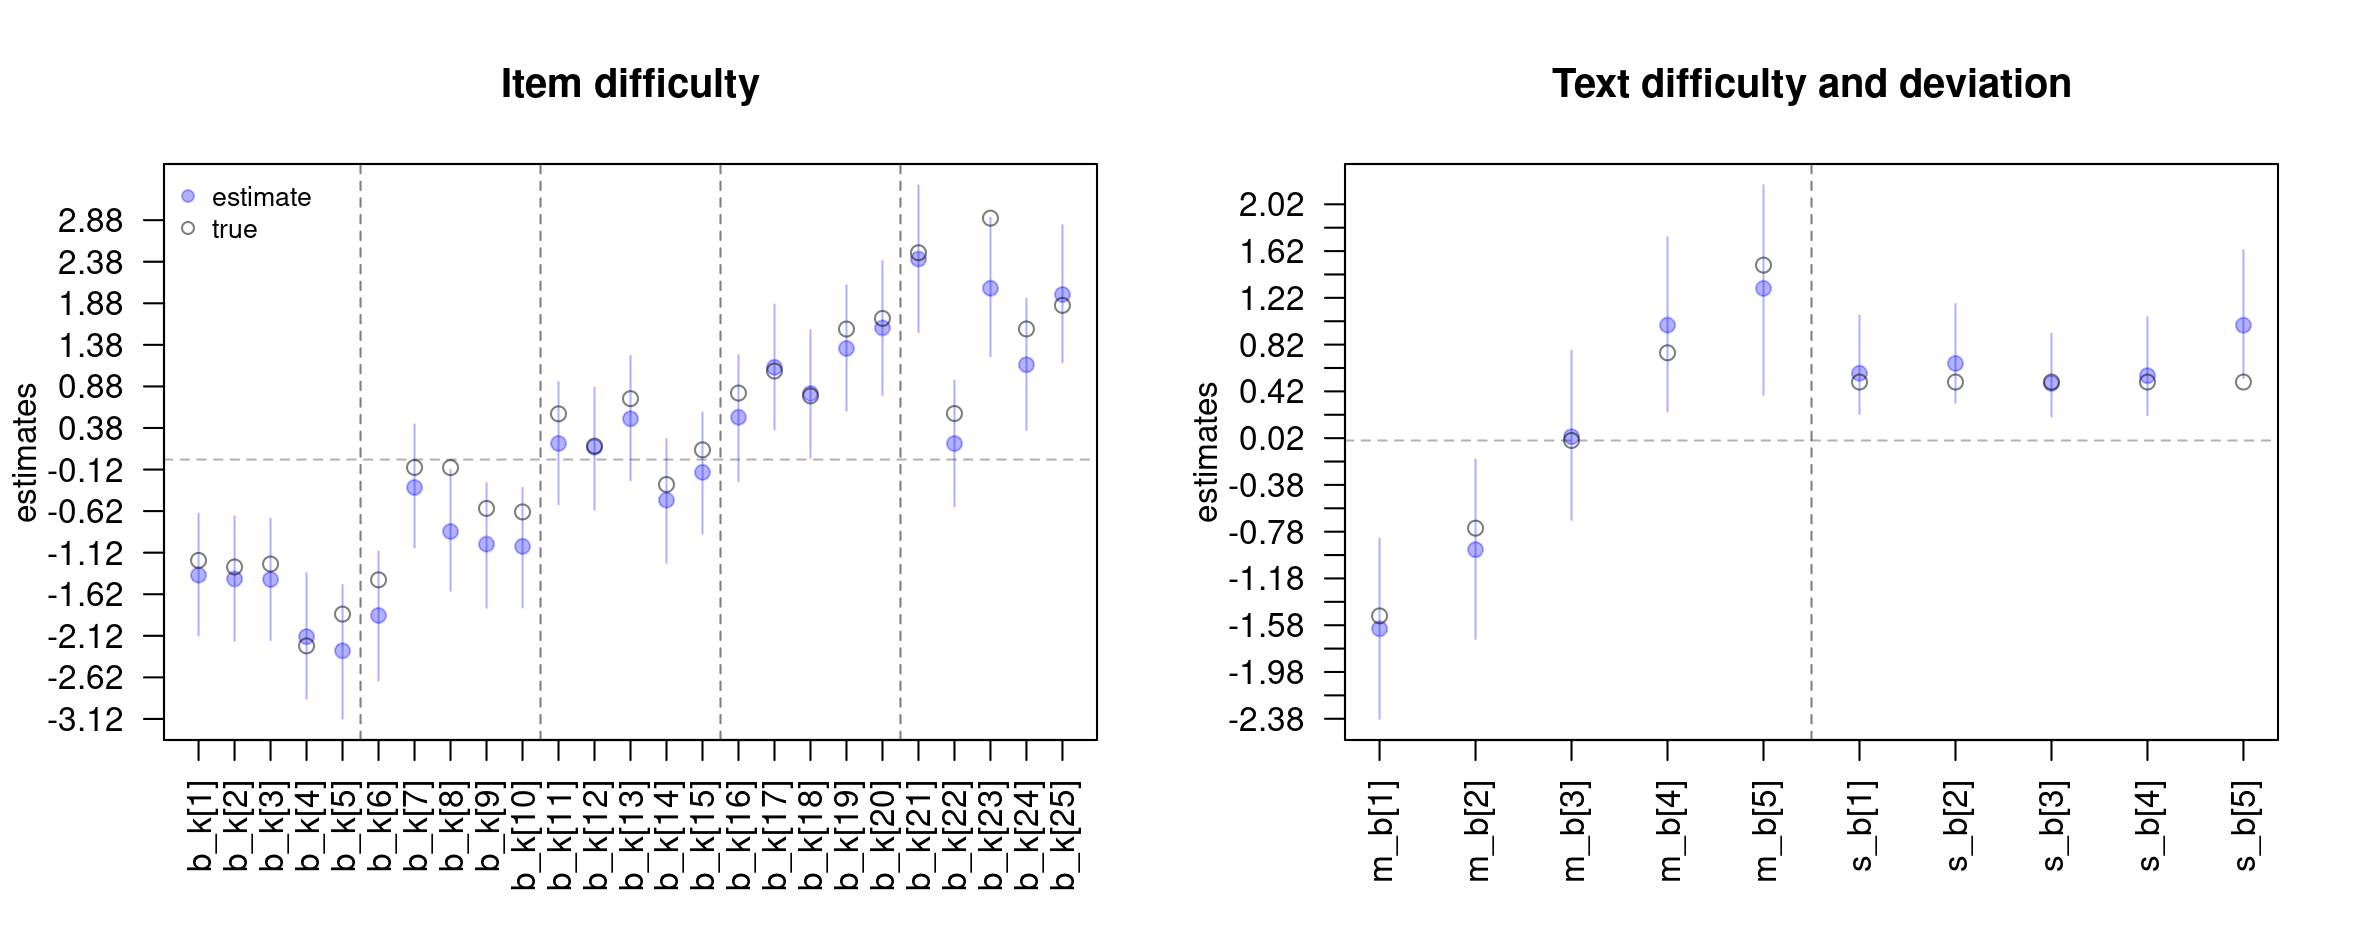
\includegraphics[width=1\linewidth]{FOLV_CE_J100_Ndata1_items}
	\end{subfigure}
	%
	\begin{subfigure}
		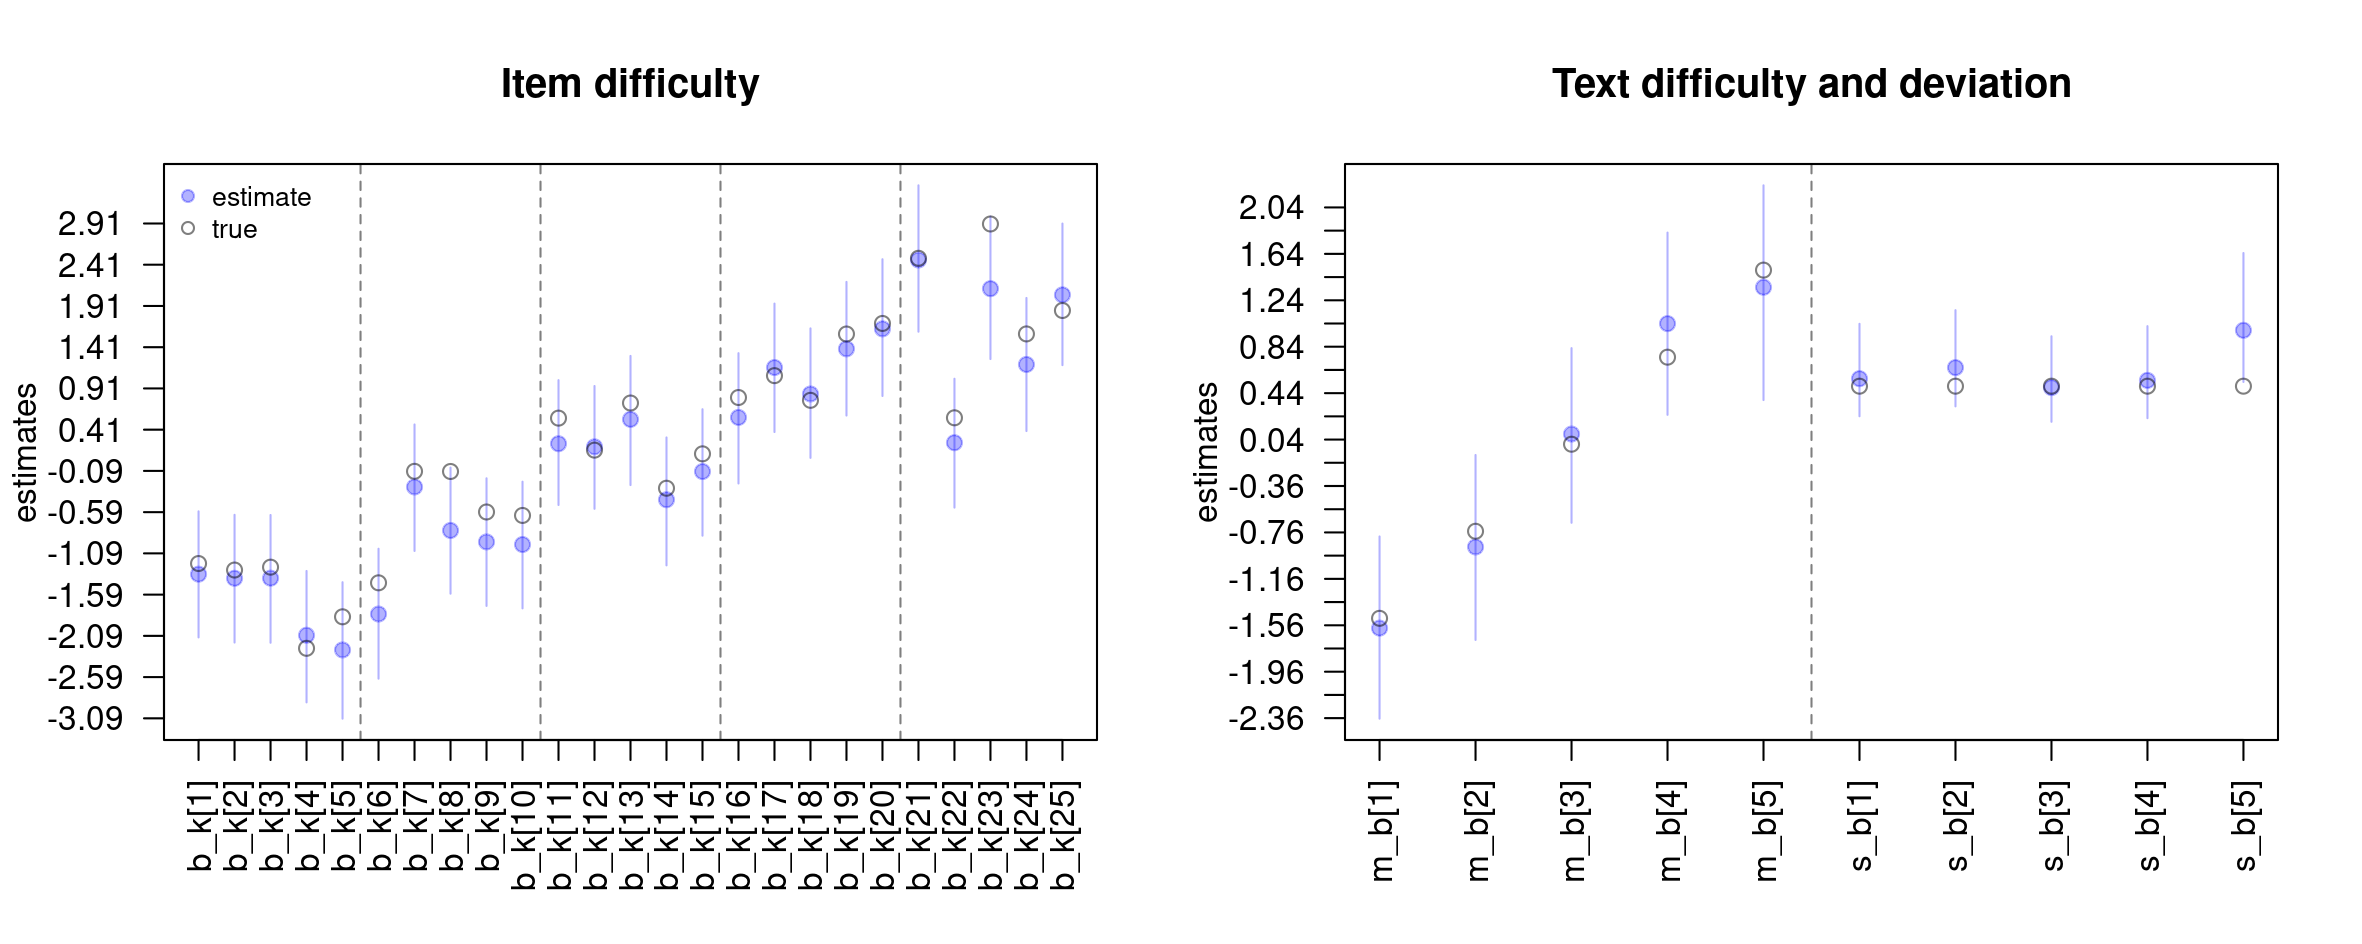
\includegraphics[width=1\linewidth]{FOLV_NC_J100_Ndata1_items}
	\end{subfigure}
	%
	\caption[First-order latent variable model (FOLV). Sample size $100$, replica $1$. Items and text parameters.]%
	{First-order latent variable model (FOLV). Sample size $100$, replica $1$. Items and text parameters. Top two panels correspond to the centered parametrization (CP). Top bottom panels correspond to the non-centered parametrization (NCP).}
	\label{fig:FOLV_recovery2}
\end{figure}
%
\begin{figure}[H]
	\centering
	\begin{subfigure}
		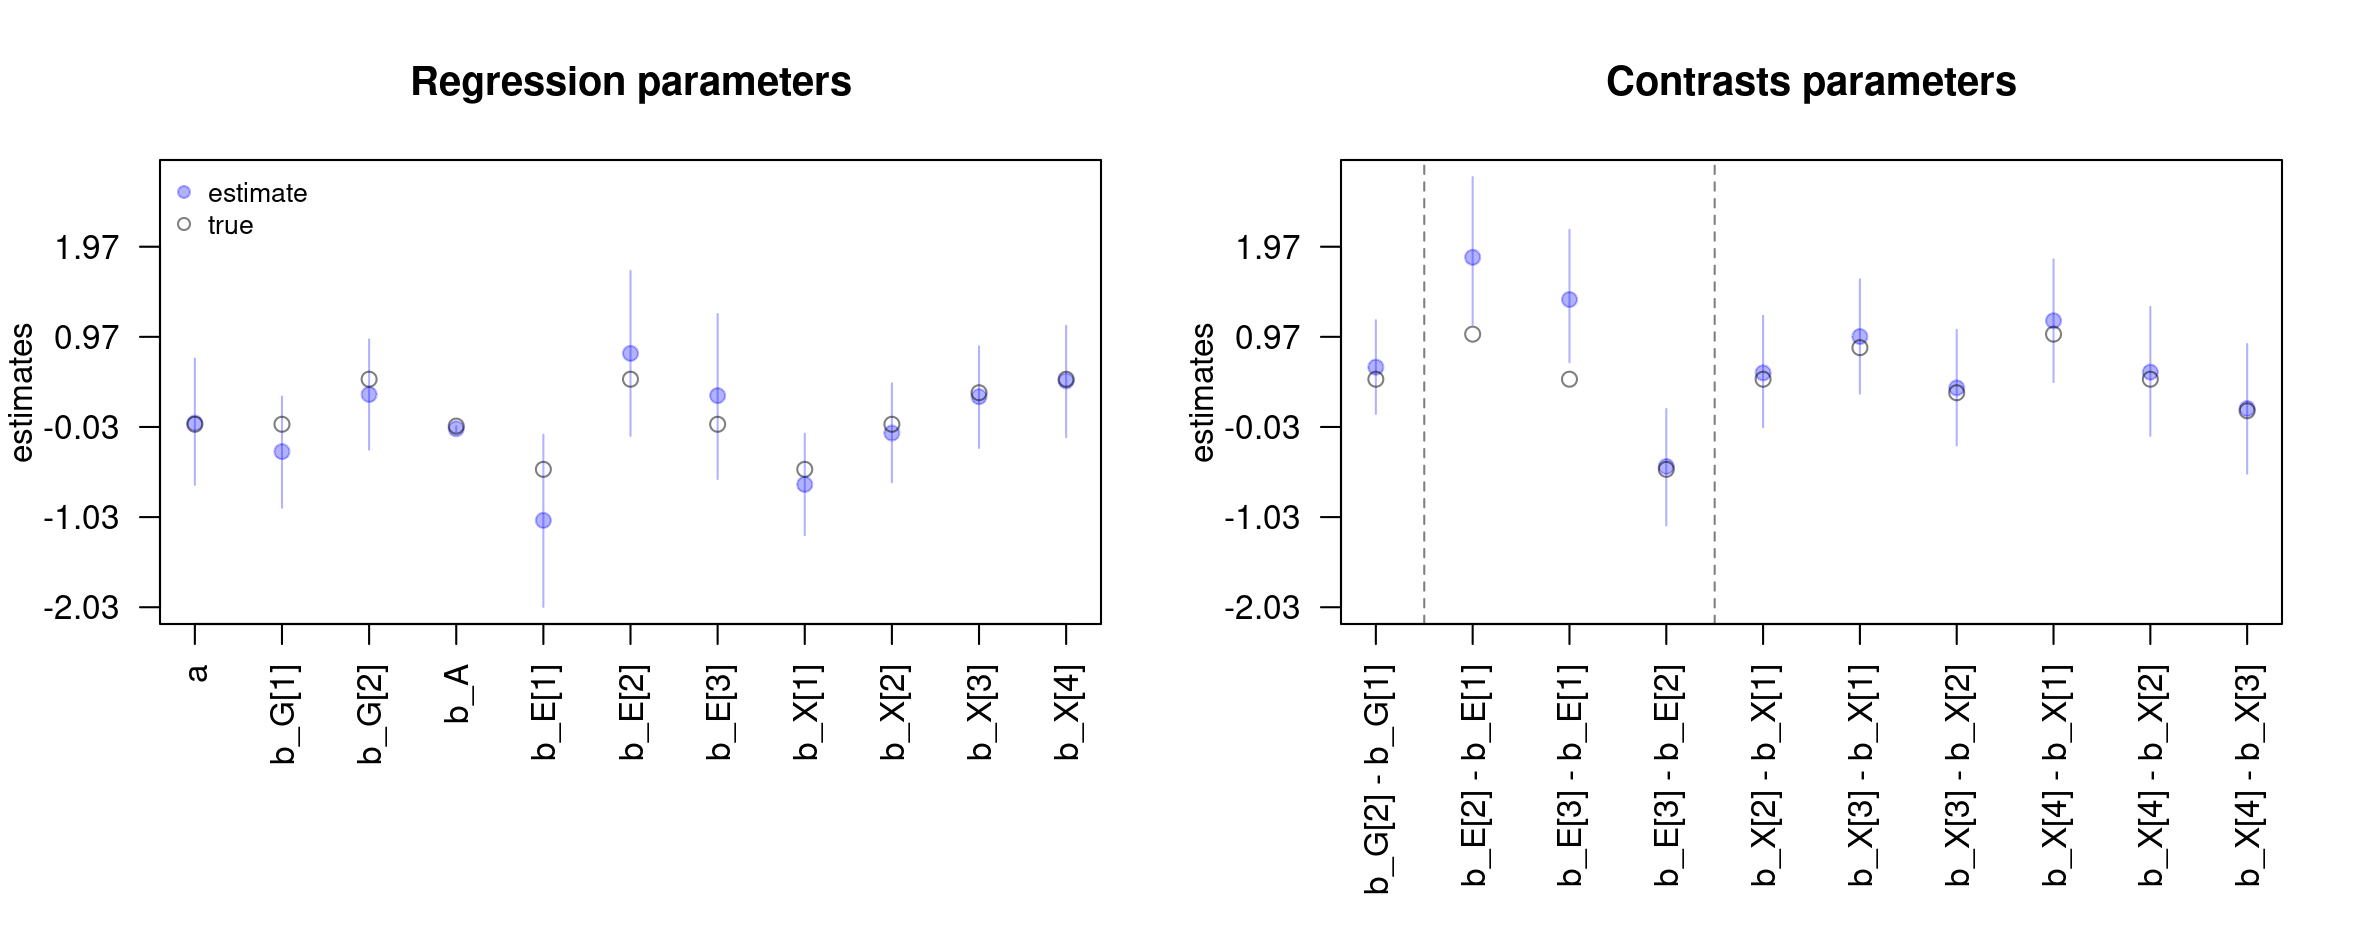
\includegraphics[width=1\linewidth]{SOLV_CE_J100_Ndata1_regression}
	\end{subfigure}
	%
	\begin{subfigure}
		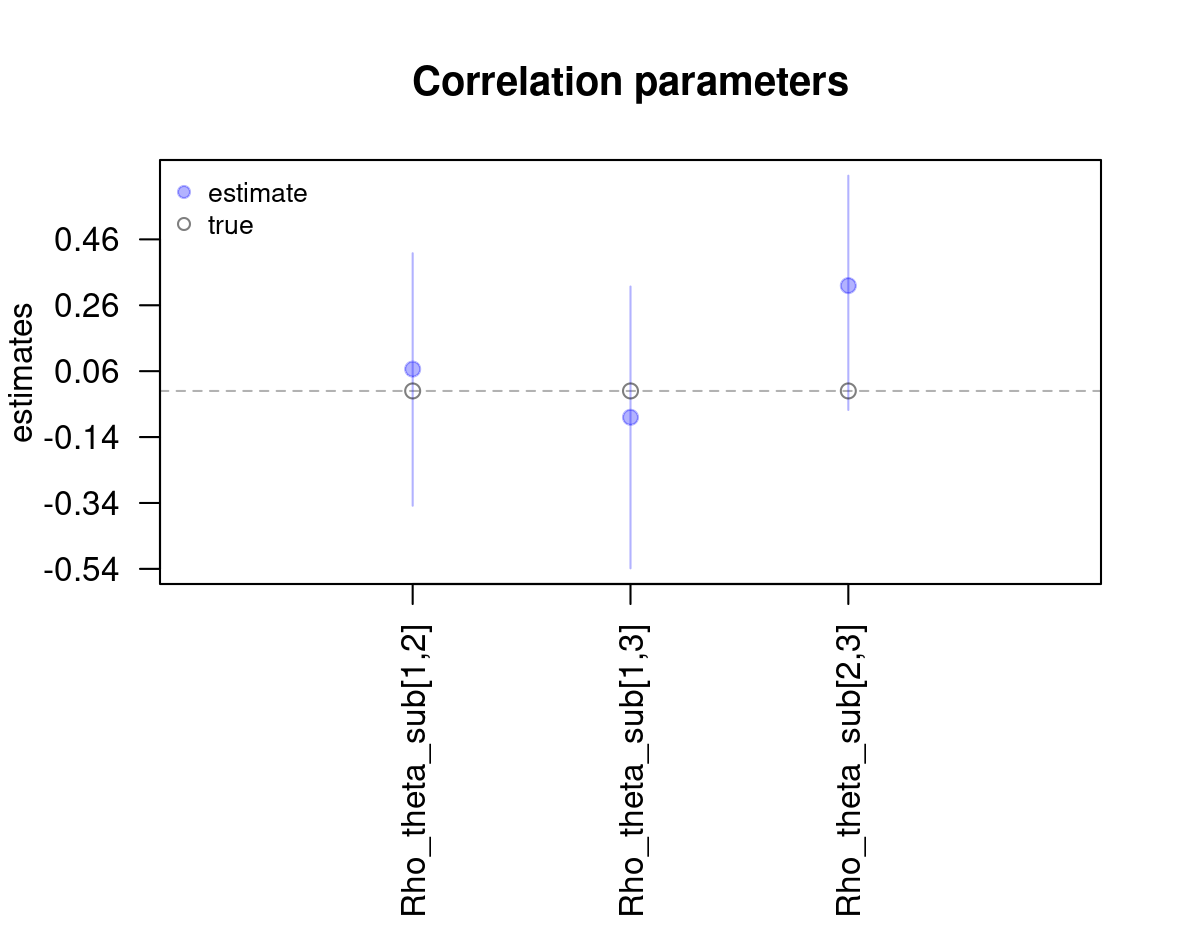
\includegraphics[width=0.48\linewidth]{SOLV_CE_J100_Ndata1_corr}
	\end{subfigure}
	%
	\begin{subfigure}
		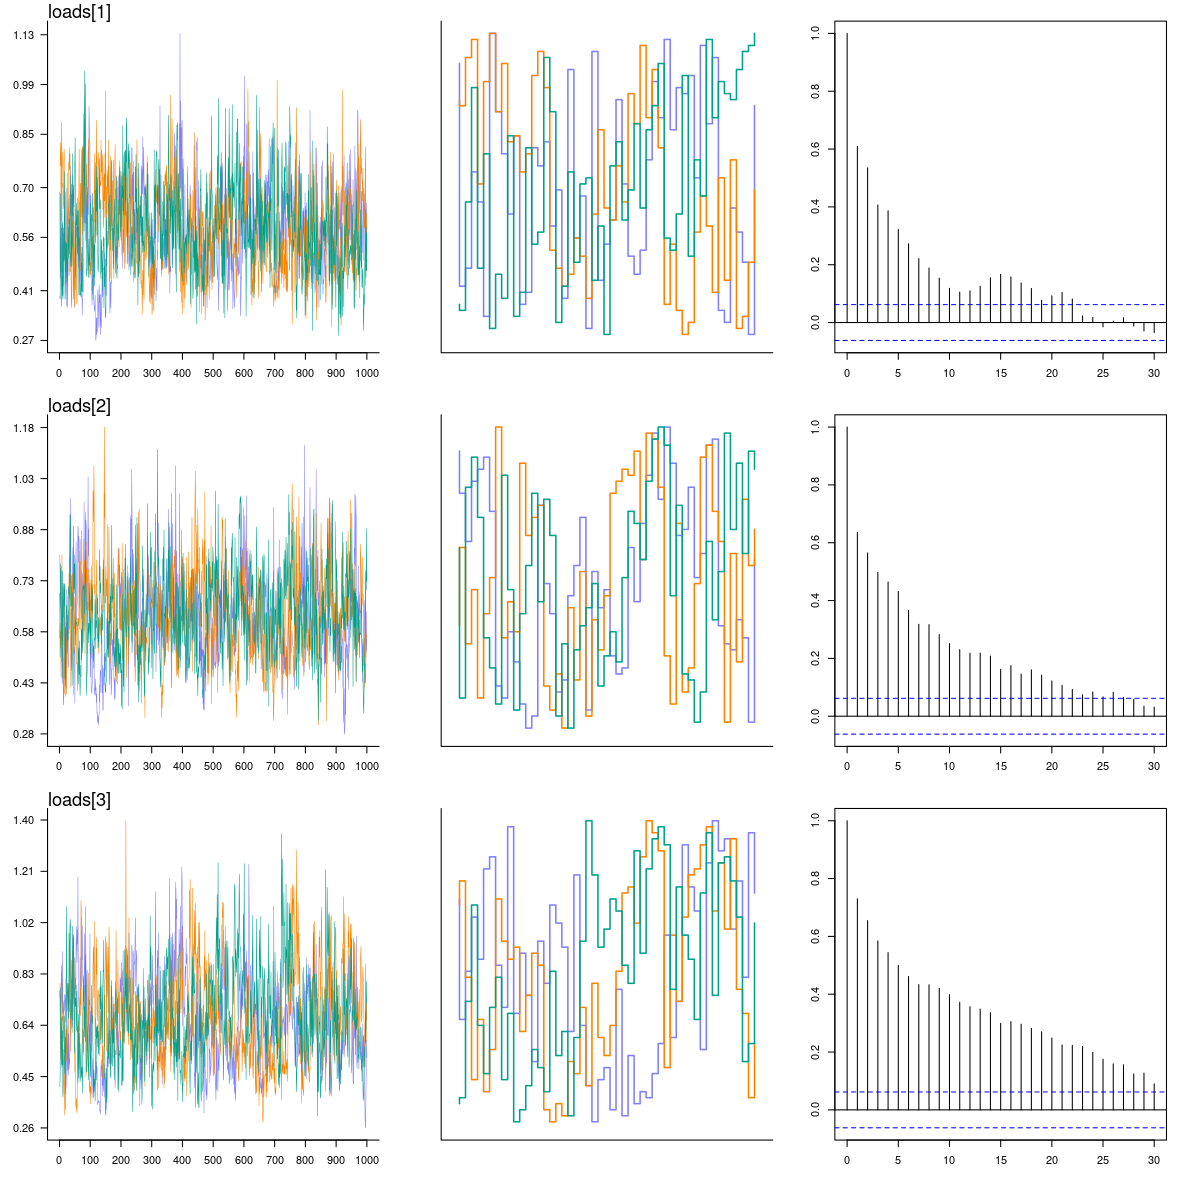
\includegraphics[width=0.48\linewidth]{SOLV_CE_J100_Ndata1_loads}
	\end{subfigure}
	%
	\caption[Second-order latent variable model (SOLV). Centered parametrization. Sample size $100$, replica $1$. Regression, contrast, correlations, and loading parameters.]%
	{Second-order latent variable model (SOLV). Centered parametrization. Sample size $100$, replica $1$. Regression, contrast, correlation, and loading parameters.}
	\label{fig:SOLV_CE_recovery1}
\end{figure}
%
\begin{figure}[H]
	\centering
	\begin{subfigure}
		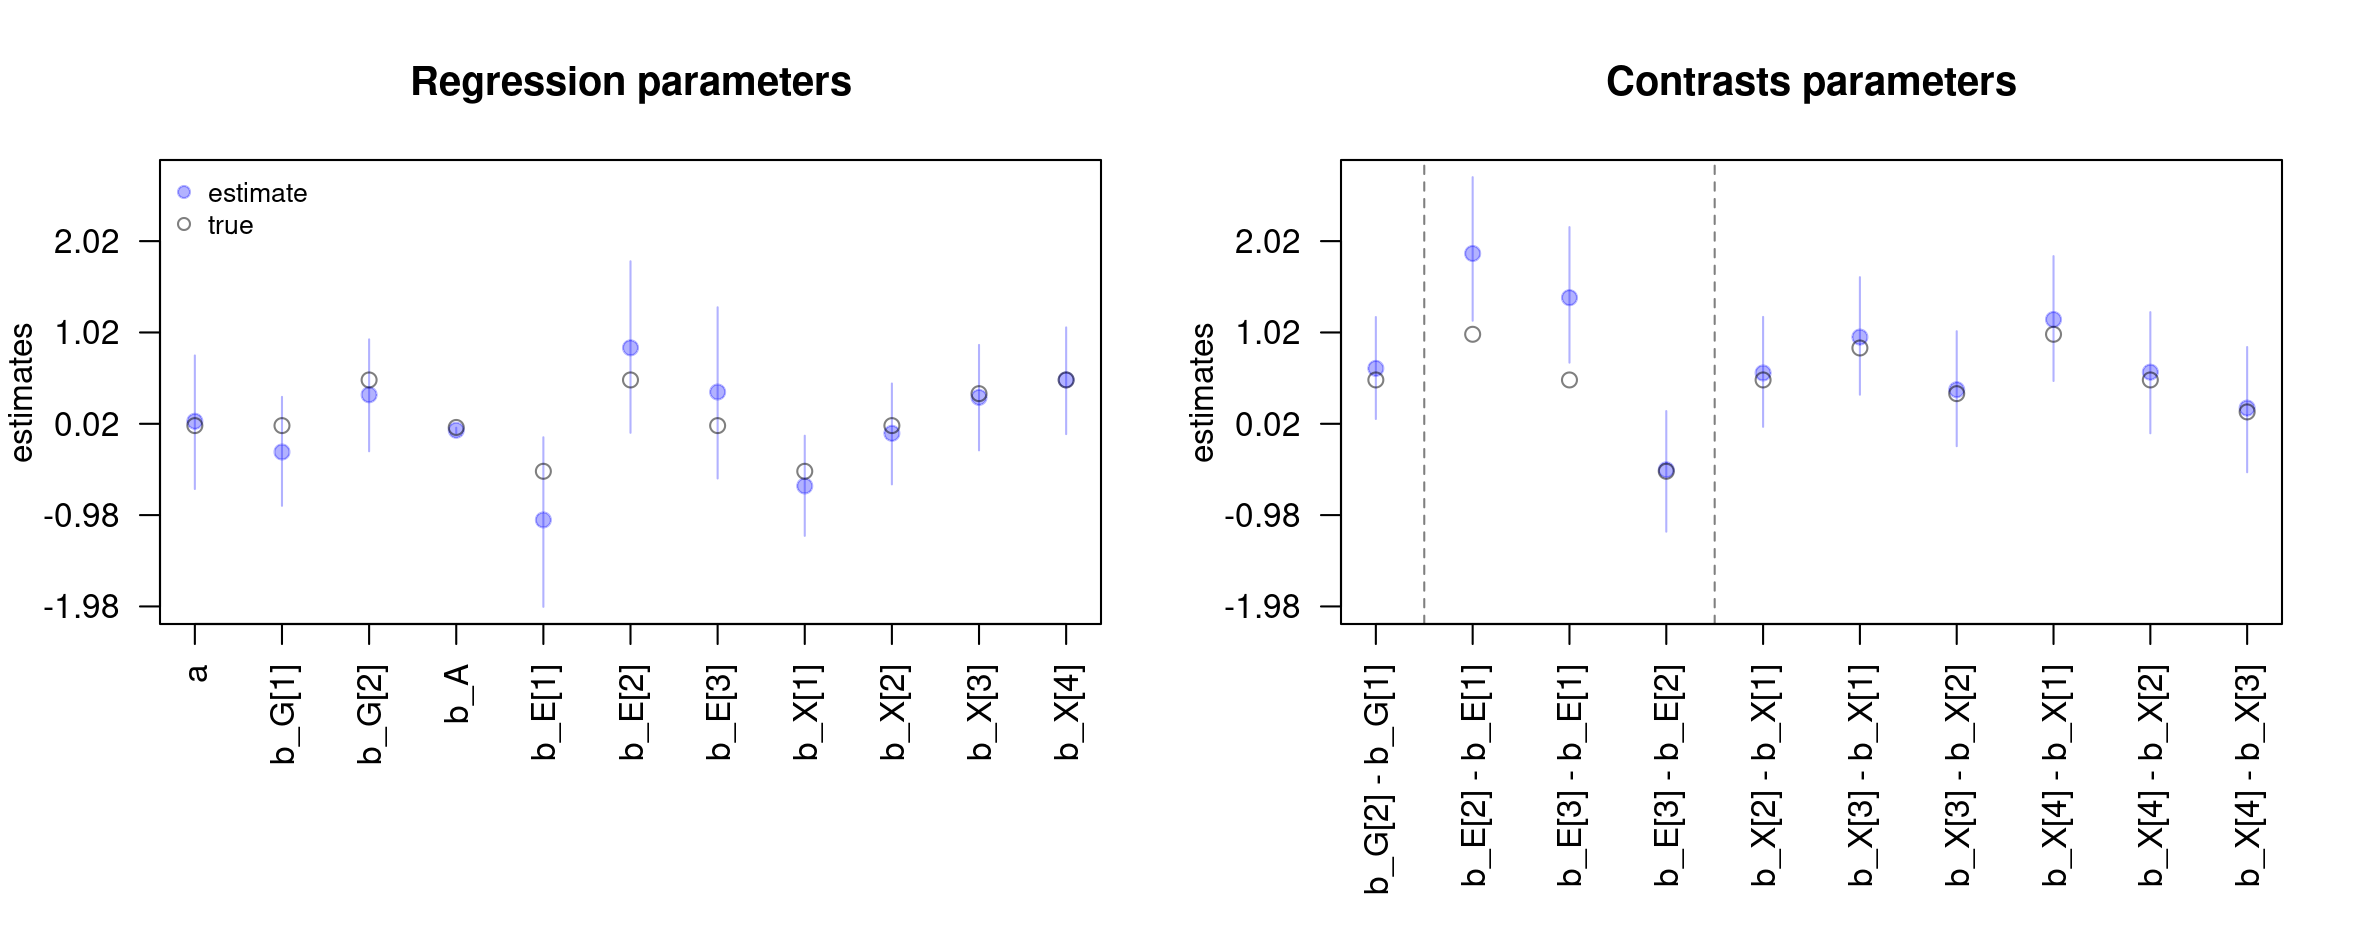
\includegraphics[width=1\linewidth]{SOLV_NC_J100_Ndata1_regression}
	\end{subfigure}
	%
	\begin{subfigure}
		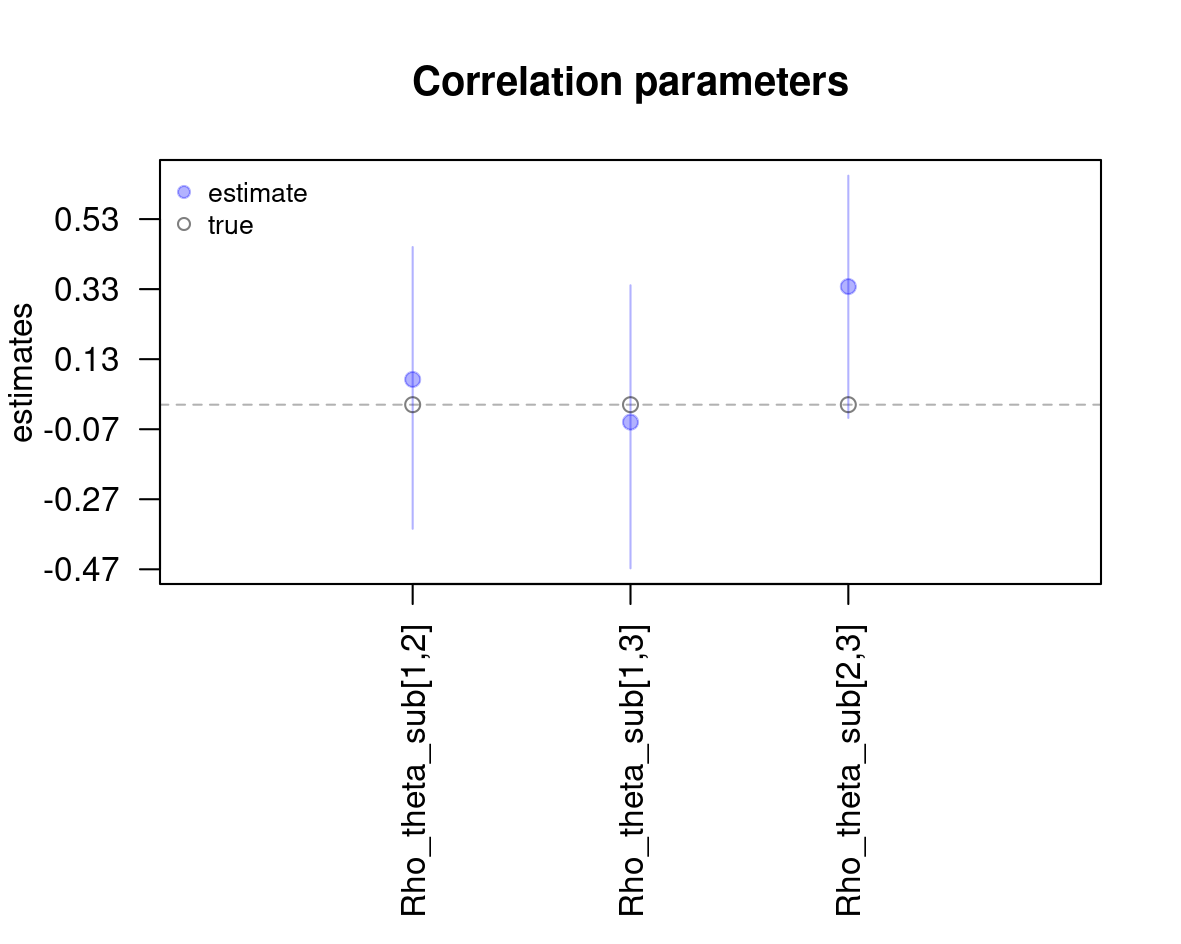
\includegraphics[width=0.48\linewidth]{SOLV_NC_J100_Ndata1_corr}
	\end{subfigure}
	%
	\begin{subfigure}
		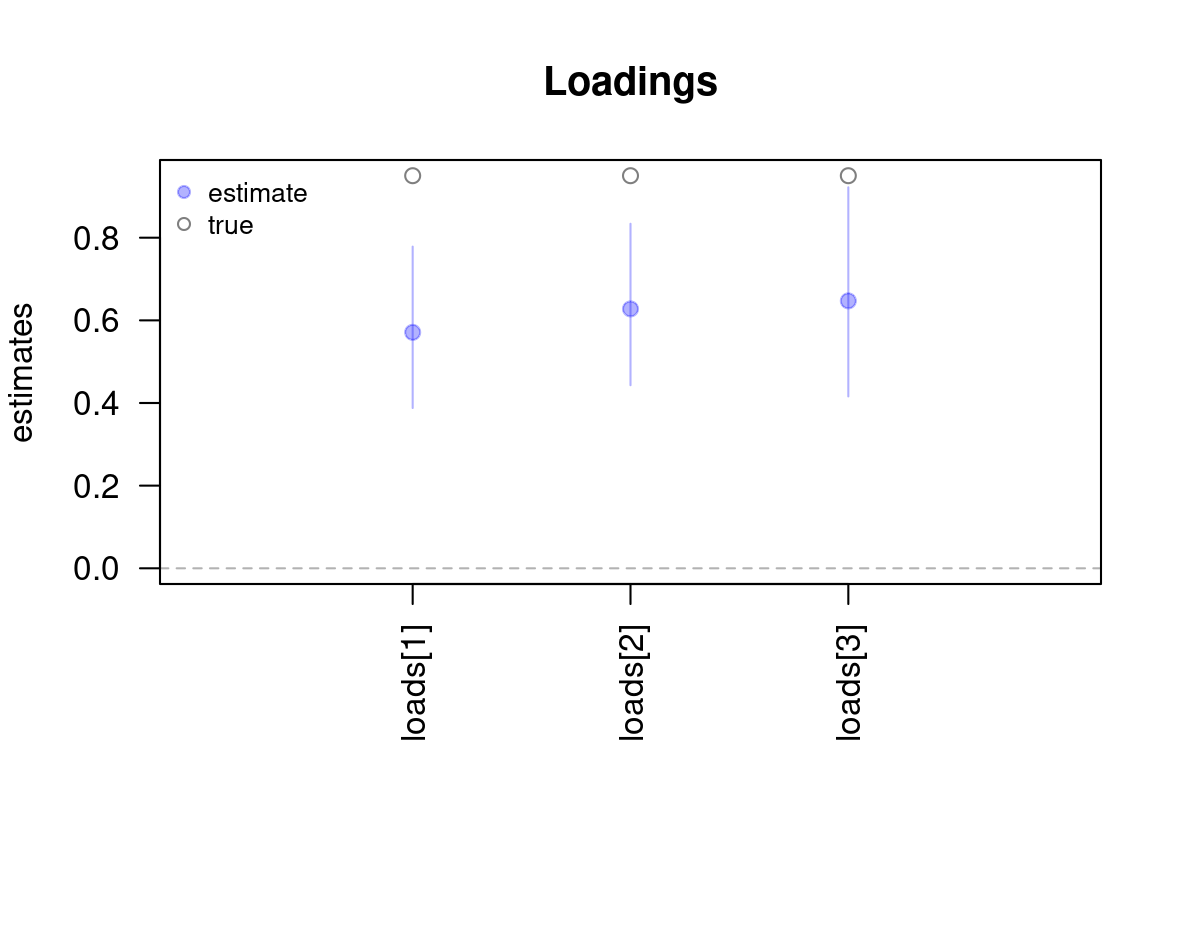
\includegraphics[width=0.48\linewidth]{SOLV_NC_J100_Ndata1_loads}
	\end{subfigure}
	%
	\caption[Second-order latent variable model (SOLV). Centered parametrization. Sample size $100$, replica $1$. Regression, contrast, correlations, and loading parameters.]%
	{Second-order latent variable model (SOLV). Centered parametrization. Sample size $100$, replica $1$. Regression, contrast, correlation, and loading parameters.}
	\label{fig:SOLV_NC_recovery1}
\end{figure}
%
\begin{figure}[H]
	\centering
	\begin{subfigure}
		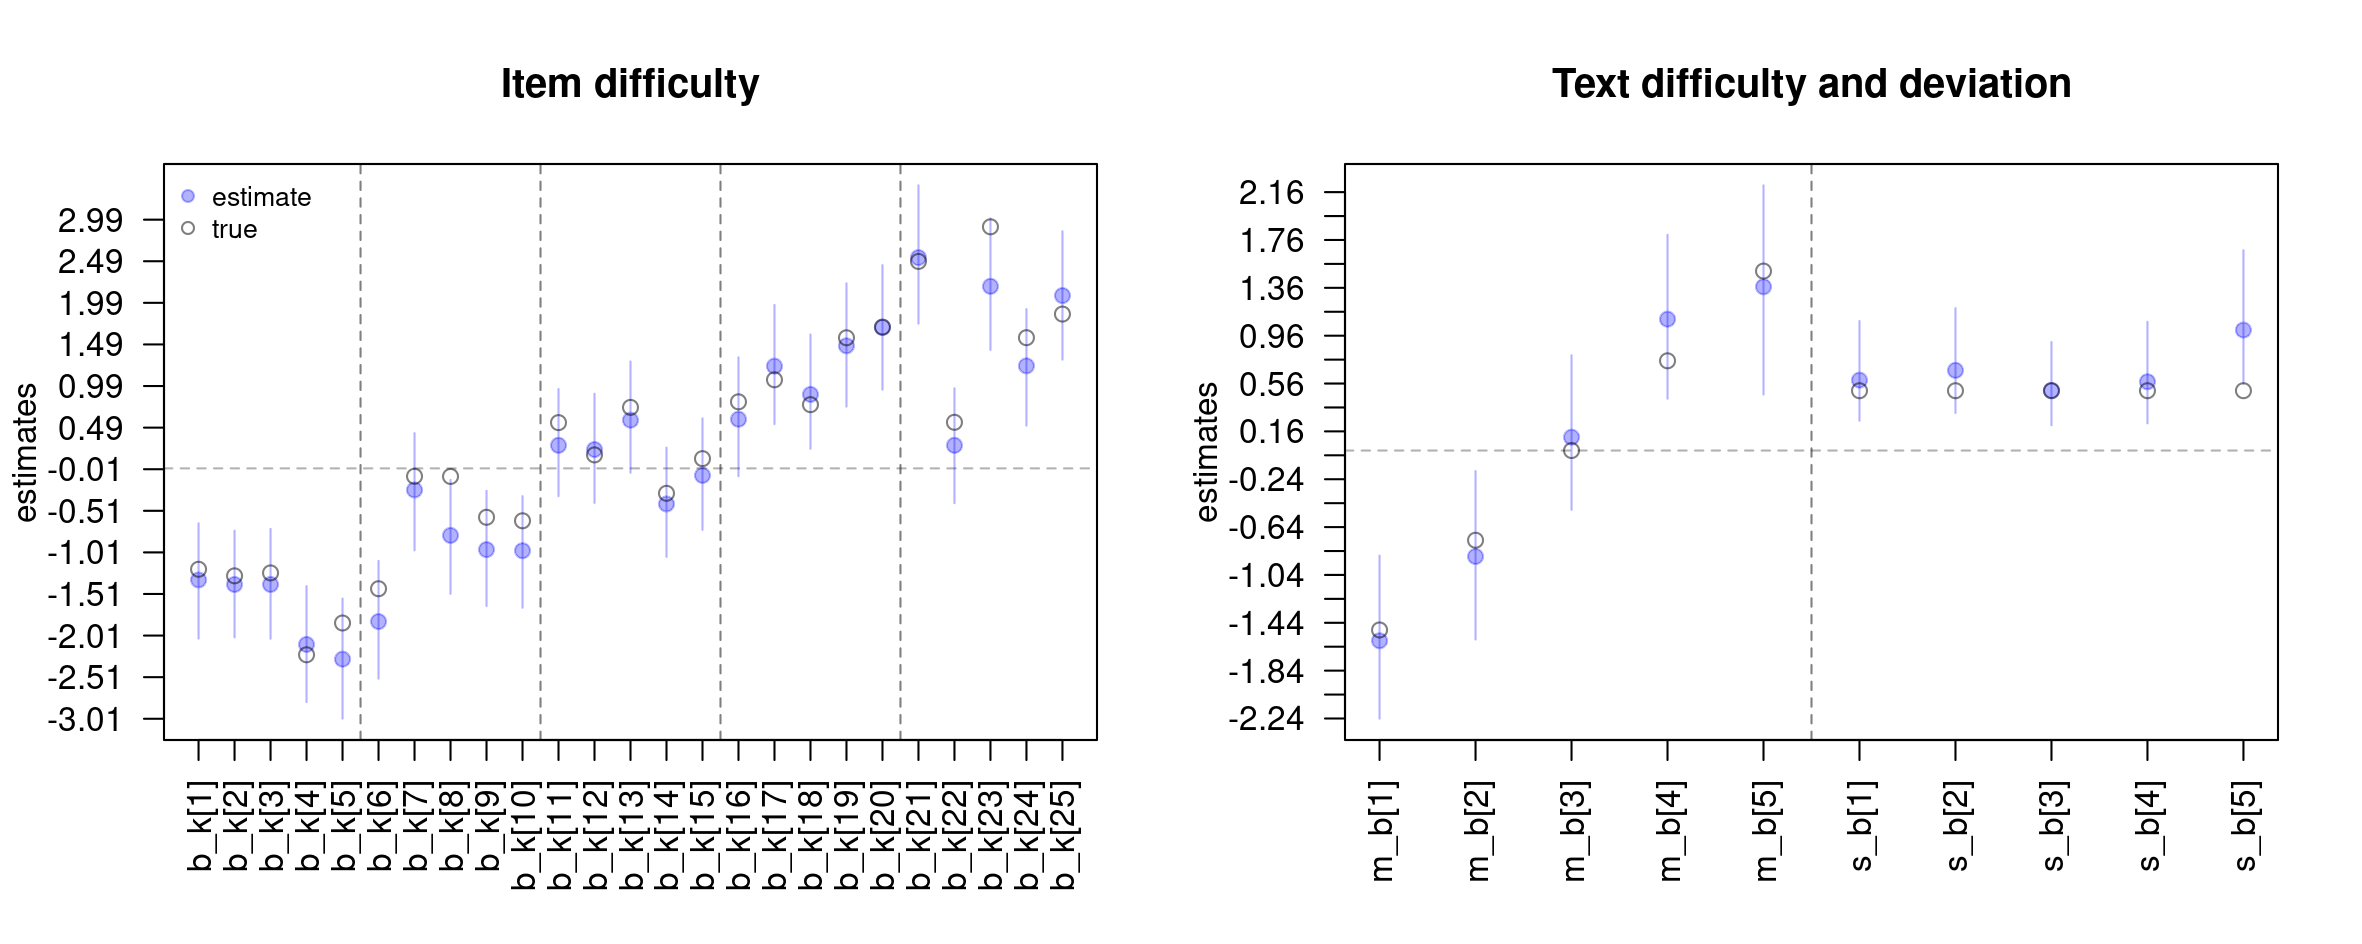
\includegraphics[width=1\linewidth]{SOLV_CE_J100_Ndata1_items}
	\end{subfigure}
	%
	\begin{subfigure}
		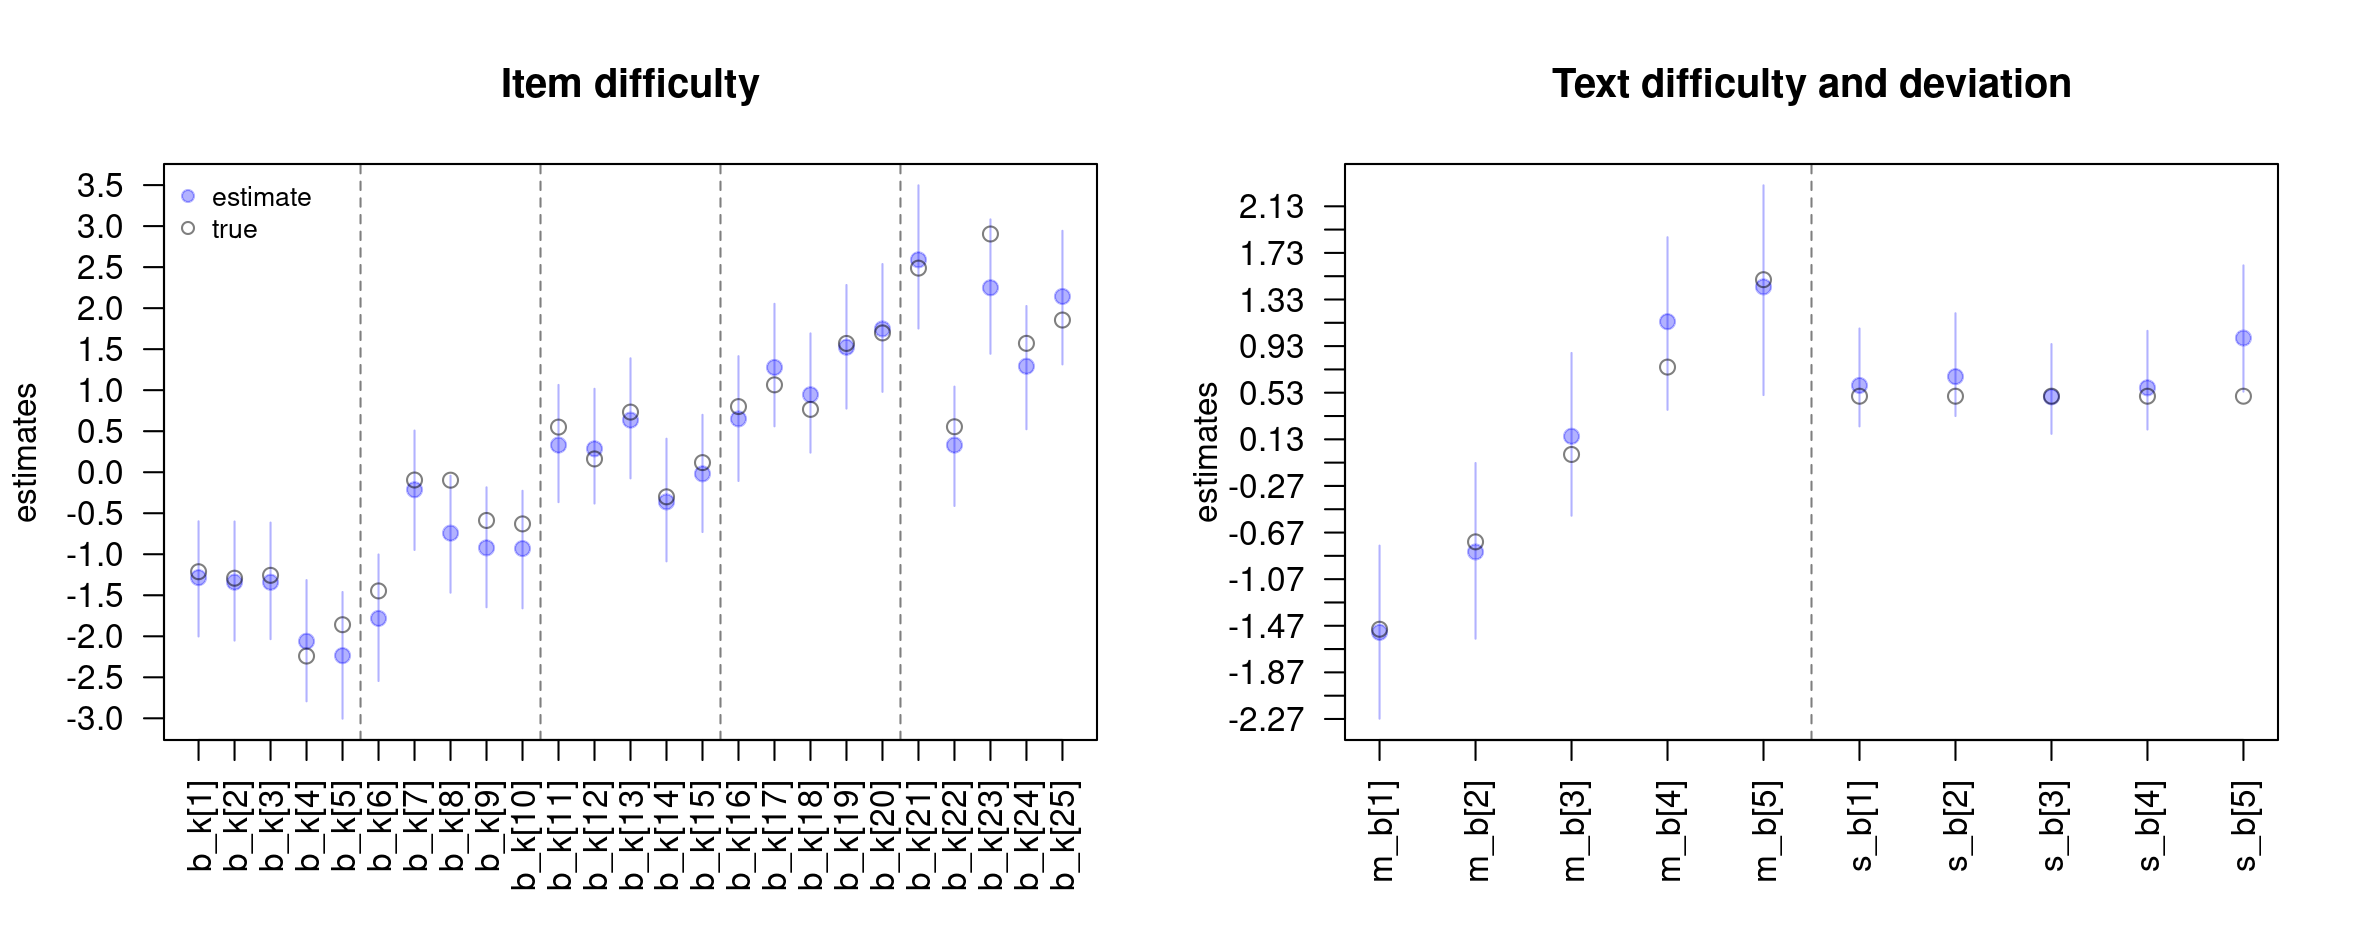
\includegraphics[width=1\linewidth]{SOLV_NC_J100_Ndata1_items}
	\end{subfigure}
	%
	\caption[First-order latent variable model (FOLV). Sample size $100$, replica $1$. Items and text parameters.]%
	{Second-order latent variable model (SOLV). Sample size $100$, replica $1$. Items and text parameters. Top two panels correspond to the centered parametrization (CP). Top bottom panels correspond to the non-centered parametrization (NCP).}
	\label{fig:SOLV_recovery2}
\end{figure}





%%%%%%%%%%%%%%%%%%%%%%%%%%%%%%%%%%%%%%%%%%%%%%%%%%%%%%%%%%%%%%%%%%%%%%%
\newpage
\subsection{Retrodictive accuracy} \label{sub_sect:retro_accuracy}

The current section shows only a small set of figures related to the retrodictive accuracy of the model. In case the reader wants to inspect the full set of figures refer to the ``retrodictive plots" image section of the accompanying github page:

\noindent \url{https://github.com/jriveraespejo/thesis/tree/master/images/retrodictive_plots} \\


On the other hand, if the reader wants to replicate or inspect the retrodictive tables refer to the ``data/tables" section of the accompanying github page:

\noindent \url{https://github.com/jriveraespejo/thesis/tree/master/data_tables} \\
%
\begin{figure}[H]
	\centering
	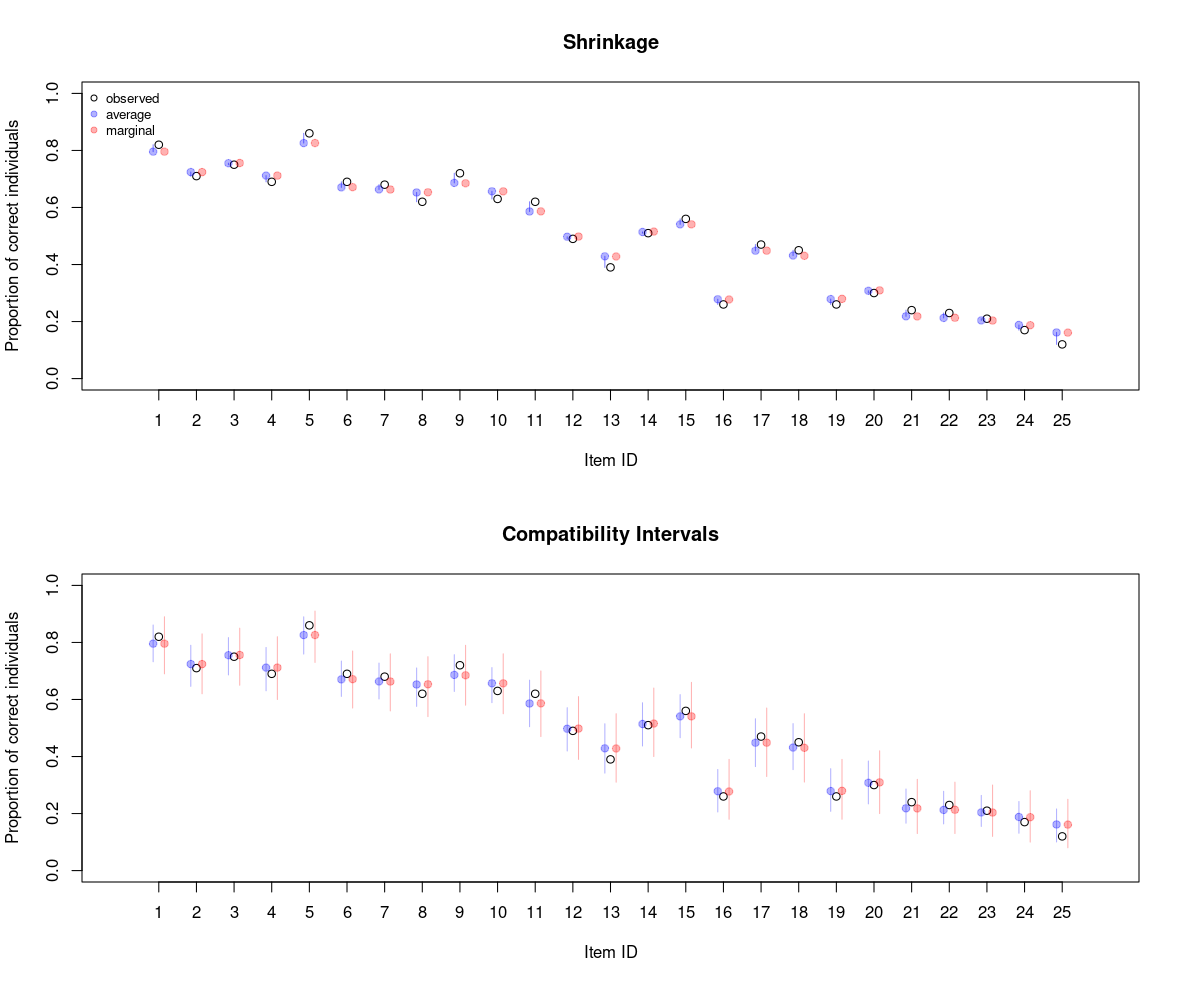
\includegraphics[width=1\linewidth]{FOLV_NC_J100_Ndata4_HitRate_items}
	%
	\caption[First-Order latent variable model (FOLV). Sample size $100$, replica number $4$. Non-centered parametrization. Items predictive plot.]%
	{First-Order latent variable model (FOLV). Sample size $100$, replica number $4$. Non-centered parametrization. Items predictive plot.}
	\label{fig:FOLV_NC_hitrate_items}
\end{figure}
%
\begin{figure}[H]
	\centering
	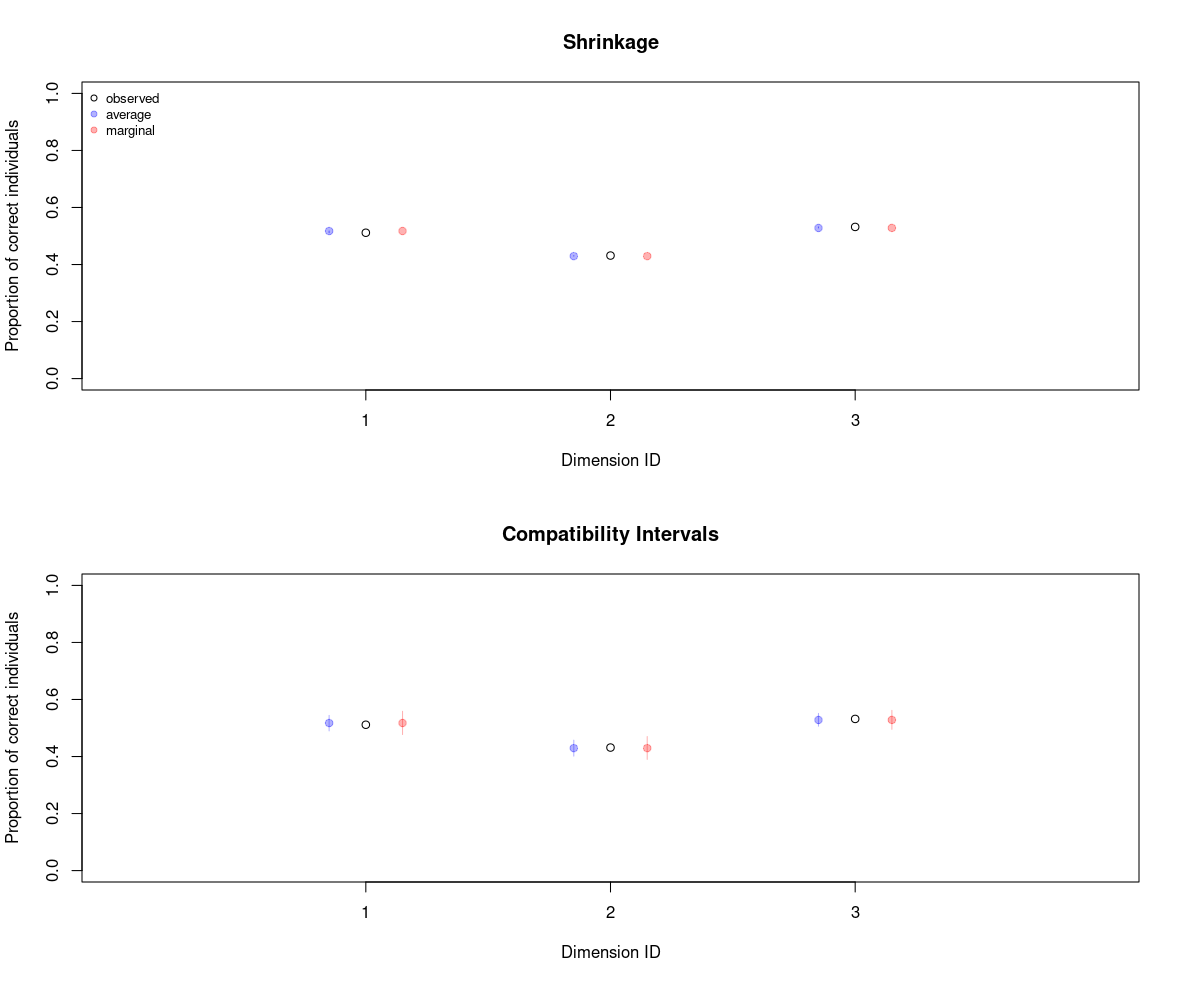
\includegraphics[width=1\linewidth]{FOLV_NC_J100_Ndata4_HitRate_dims}
	%
	\caption[First-Order latent variable model (FOLV). Sample size $100$, replica number $4$. Non-centered parametrization. Dimension predictive plot.]%
	{First-Order latent variable model (FOLV). Sample size $100$, replica number $4$. Non-centered parametrization. Dimension predictive plot.}
	\label{fig:FOLV_NC_hitrate_dim}
\end{figure}
%
\begin{figure}[H]
	\centering
	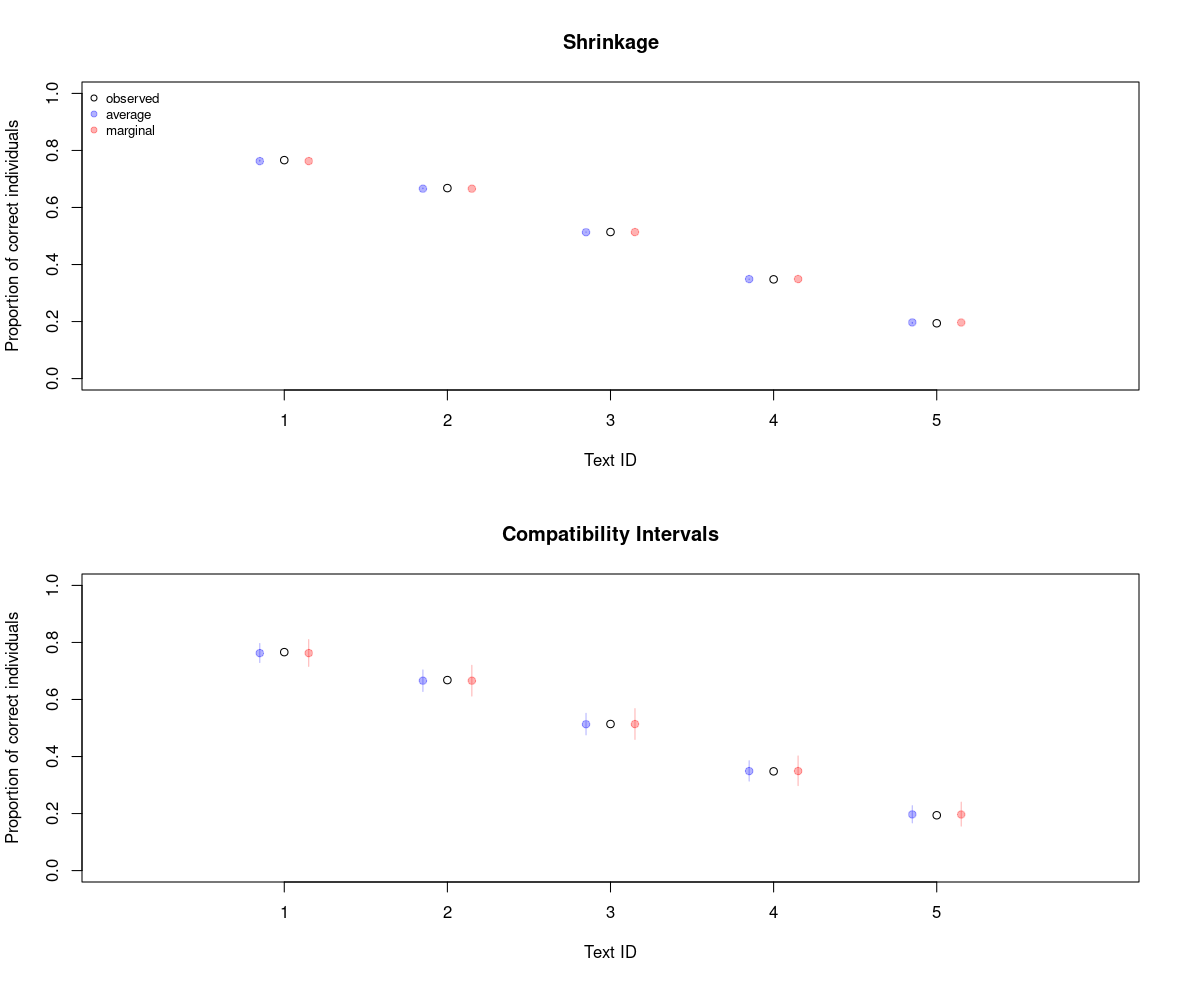
\includegraphics[width=1\linewidth]{FOLV_NC_J100_Ndata4_HitRate_texts}
	%
	\caption[First-Order latent variable model (FOLV). Sample size $100$, replica number $4$. Non-centered parametrization. Text predictive plot.]%
	{First-Order latent variable model (FOLV). Sample size $100$, replica number $4$. Non-centered parametrization. Text predictive plot.}
	\label{fig:FOLV_NC_hitrate_text}
\end{figure}
%
\begin{figure}[H]
	\centering
	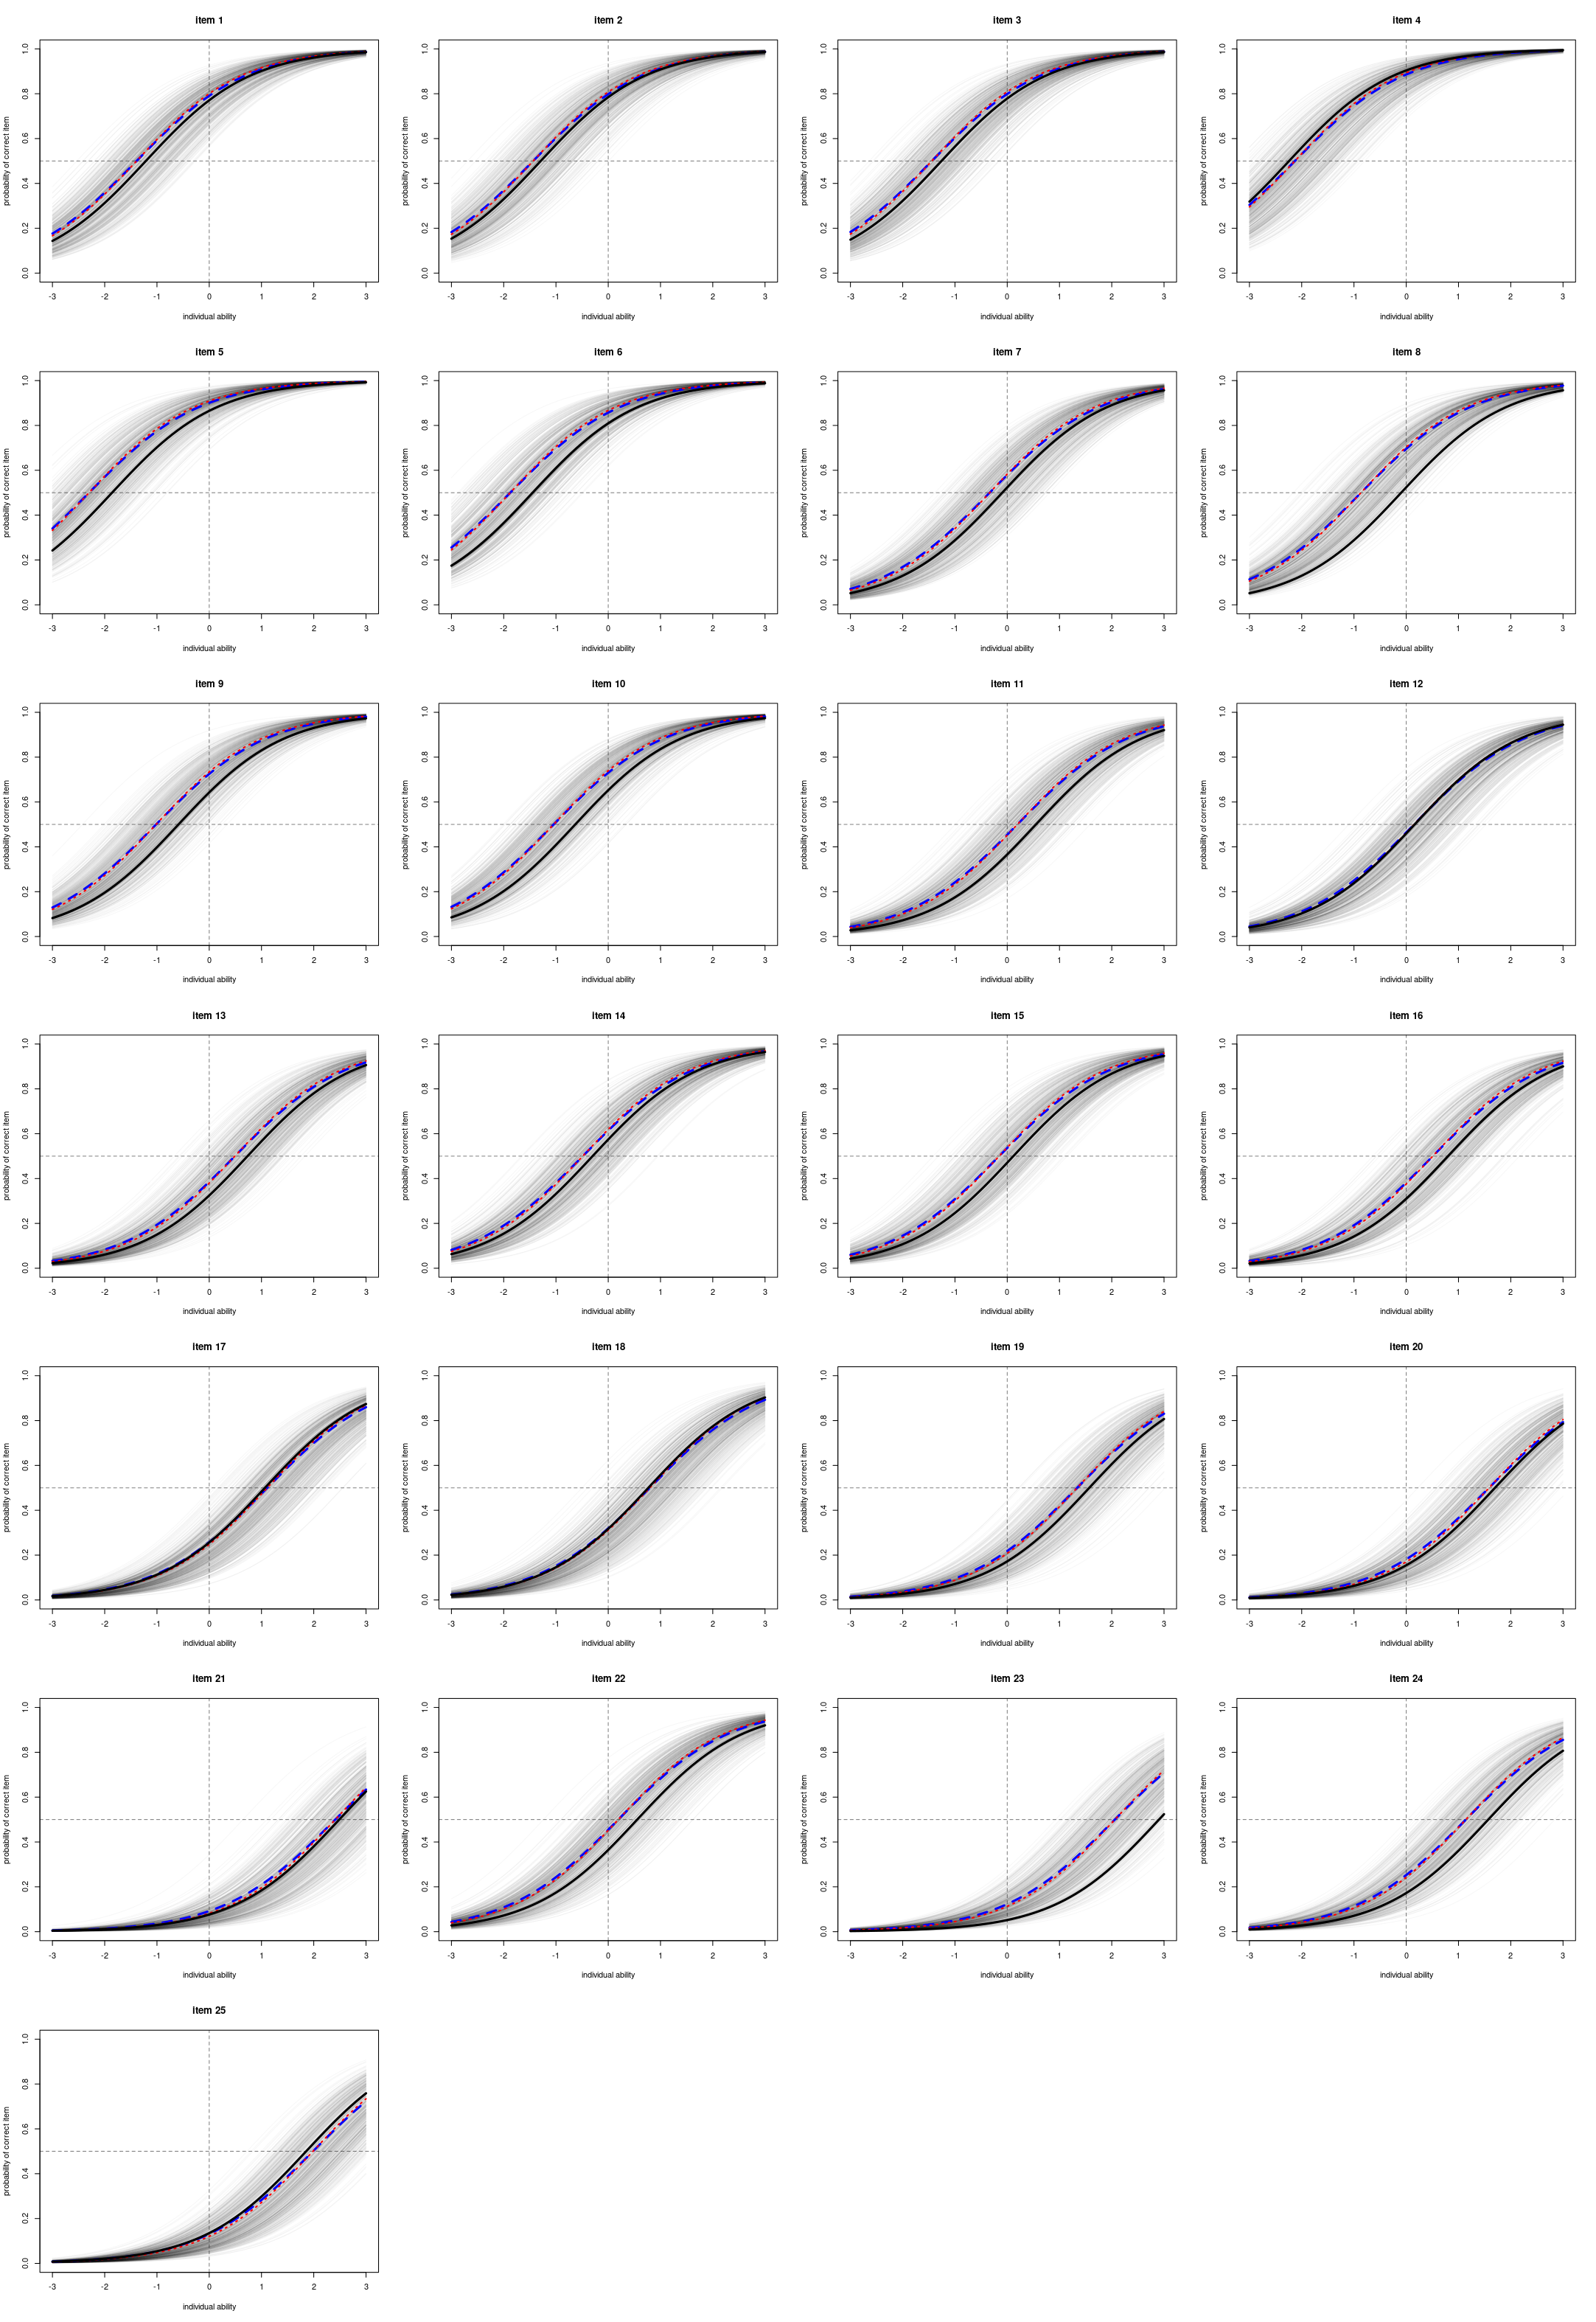
\includegraphics[width=0.95\linewidth]{FOLV_CE_J100_Ndata1_ICC}
	%
	\caption[First-Order latent variable model (FOLV). Sample size $100$, replica number $4$. Centered parametrization. Item characteristic curves (ICC).]%
	{First-Order latent variable model (FOLV). Sample size $100$, replica number $4$. Centered parametrization. Item characteristic curves (ICC)}
	\label{fig:FOLV_CE_ICC}
\end{figure}
%
\begin{figure}[H]
	\centering
	\includegraphics[width=0.95\linewidth]{FOLV_CE_J100_Ndata1_IIF}
	%
	\caption[First-Order latent variable model (FOLV). Sample size $100$, replica number $4$. Non-centered parametrization. Item information function (IIF).]%
	{First-Order latent variable model (FOLV). Sample size $100$, replica number $4$. Non-centered parametrization. Item information function (IIF).}
	\label{fig:FOLV_CE_IIF}
\end{figure}